\chapter{Magnets, superconductors, Dirac materials and defects}\label{chap:7}
\chaptermark{Magnets, superconductors, Dirac materials, defects}% short running head

Silicon offers dark matter two kinds of excitation: an electron lifted across the \SI{1.17}{eV} gap, and phonons up to \SI{64}{meV}. A particle that couples to the spin of the electron has no cheaper excitation in silicon, since every spin is paired in a bond and flipping one costs the gap. Other solids have excitations below these energies or of other kinds. In NiO the spins of the nickel ions order, and a particle that couples to spin can create a quantum of their precession, a magnon. In a superconductor such as aluminum the electrons at the Fermi surface bind into pairs, and breaking a pair costs only twice the superconducting gap. Dirac materials, whose electrons obey a Dirac equation with a velocity far below that of light, offer pair excitations across a gap much smaller than that of silicon. Donors and color centers put bound levels inside the gap of silicon itself, shallow for a donor and deep for a color center, and a struck atom can leave a defect that stores energy. Each of these targets is built largely from pieces already in hand: the exchange term of the Coulomb interaction (\cref{sec:2.3}), the electron--phonon coupling (\cref{chap:6}), the $\vect{k}\cdot\vect{p}$ expansion (\cref{sec:3.3}) and the hydrogenic envelope (\cref{sec:4.9}). The rest is physics that silicon does not have, above all spontaneously broken symmetry, which brings with it collective modes and quasiparticles whose energies are set by an interaction rather than by a band gap. We will derive, for each target, the excitation spectrum and the response that the rate formulas of the later chapters take as input.

\section{Magnetic order and spin waves}\label{sec:7.1}

Each nickel ion in NiO carries a spin, and below \SI{523}{K}, the measured Néel temperature~\cite[Table~IV]{fischer2009exchange}, the spins order: those in one $(111)$ plane of the crystal point one way, those in the next plane the opposite way. A disturbance of that order travels through the crystal as a spin wave. The quanta of spin waves, the \emph{magnons}, have energies up to ${\sim}\SI{117}{meV}$. Inelastic neutron scattering at \SI{78}{K} measured their dispersion, with an initial slope of ${\sim}\SI{250}{meV.\angstrom}$~\cite{hutchings1972measurement}. In an ordered magnet a particle that couples to the spin of the electron can create a magnon~\cite{trickle2020detecting}. The energy deposits then run from a few meV to about a tenth of an eV. To compute the rate of magnon creation we need the interaction that orders the spins, the spectrum of the spin waves, and the operator through which a probe creates magnons.

\subsection{Exchange and the Heisenberg model}

The Coulomb interaction does not act on spin, yet it makes the energy of two electrons depend on how their spins are aligned. Put one electron in each of two orthogonal orbitals $\varphi_a$ and $\varphi_b$. In the spin triplet the spatial wavefunction is antisymmetric, $[\varphi_a(\vect{r})\varphi_b(\vect{r}') - \varphi_b(\vect{r})\varphi_a(\vect{r}')]/\sqrt2$, and in the singlet it is symmetric. The expectation value of the Coulomb repulsion $v_{\mathrm{C}}(\vect{r} - \vect{r}')$ is then $C \mp K_{\mathrm{ex}}$, upper sign for the triplet, with the direct integral $C$ and the exchange integral
\begin{equation}
  K_{\mathrm{ex}} = \int\dd^3r\,\dd^3r'\,\varphi_a^*(\vect{r})\varphi_b^*(\vect{r}')\,v_{\mathrm{C}}(\vect{r} - \vect{r}')\,\varphi_b(\vect{r})\varphi_a(\vect{r}') .
  \label{eq:7.1-Kex}
\end{equation}
The exchange integral $K_{\mathrm{ex}}$ is the exchange term of \cref{eq:2.3-direct-exchange}, written for localized orbitals instead of plane waves. It is the Coulomb self-energy of the charge distribution $\varphi_a^*\varphi_b$, and since the Fourier transform $v_{\mathrm{C}}(k) = e^2/k^2$ is positive, $K_{\mathrm{ex}} > 0$. The triplet therefore lies $2K_{\mathrm{ex}}$ below the singlet: parallel spins keep the electrons apart and save Coulomb energy. The resulting preference for parallel spins is Hund's rule, and within one Ni$^{2+}$ ion it aligns the two holes of the $3d$ shell into a spin $|\vect{S}| = 1$.

The four spin states can be described without any reference to orbitals. With $\vect{S}_1\cdot\vect{S}_2 = \frac12[(\vect{S}_1 + \vect{S}_2)^2 - \vect{S}_1^2 - \vect{S}_2^2]$, which is $-\frac34$ in the singlet and $\frac14$ in the triplet, the operator
\begin{equation}
  H_{12} = E_{\mathrm{orb}} + C - \tfrac12K_{\mathrm{ex}} - 2K_{\mathrm{ex}}\,\vect{S}_1\cdot\vect{S}_2
  \label{eq:7.1-dirac}
\end{equation}
has the singlet energy $E_{\mathrm{orb}} + C + K_{\mathrm{ex}}$ and the triplet energy $E_{\mathrm{orb}} + C - K_{\mathrm{ex}}$, with $E_{\mathrm{orb}}$ the sum of the two one-electron orbital energies. The Coulomb interaction depends only on the positions of the electrons, and through exchange it has become a coupling between their spins, of strength $-2K_{\mathrm{ex}}$ and ferromagnetic sign.

\paragraph{Kinetic exchange.} Between electrons on neighboring ions of an insulator, however, a second mechanism usually dominates, and it has the opposite sign. Take two sites with one orbital each and the hopping $t_{\mathrm{hop}} > 0$ of the tight-binding model of \cref{sec:3.2}. Putting two electrons on the same site costs the on-site or Hubbard repulsion $U_{\mathrm{H}}$:
\begin{equation}
  H = -t_{\mathrm{hop}}\sum_{s}\bigl(c^\dagger_{1s}c_{2s} + c^\dagger_{2s}c_{1s}\bigr) + U_{\mathrm{H}}\sum_{i=1,2}c^\dagger_{i\uparrow}c_{i\uparrow}\,c^\dagger_{i\downarrow}c_{i\downarrow} .
  \label{eq:7.1-hubbard}
\end{equation}
With two electrons and $t_{\mathrm{hop}} = 0$, the four states with one electron on each site are degenerate at zero energy, and the two doubly occupied states lie at $U_{\mathrm{H}}$. The hopping connects the singly occupied states with the doubly occupied ones. A triplet cannot hop, since the Pauli principle forbids two parallel spins in one orbital: for the state $c^\dagger_{1\uparrow}c^\dagger_{2\uparrow}|0\rangle$ the hop is blocked directly, and the other two members of the triplet follow by rotational symmetry. The triplet stays at zero energy to all orders. The singlet couples to the symmetric combination of the doubly occupied states, through two hops (from site 1 or from site 2) that add, with a matrix element of magnitude $2t_{\mathrm{hop}}$. To second order in $t_{\mathrm{hop}}/U_{\mathrm{H}}$ its energy is $-(2t_{\mathrm{hop}})^2/U_{\mathrm{H}}$. As \cref{eq:7.1-dirac} shows, the coefficient of $\vect{S}_1\cdot\vect{S}_2$ is the triplet energy minus the singlet energy. With both mechanisms present the coefficient is
\begin{equation}
  J^{\mathrm{ex}} = \frac{4t_{\mathrm{hop}}^2}{U_{\mathrm{H}}} - 2K_{\mathrm{ex}} .
  \label{eq:7.1-superexchange}
\end{equation}
The picture behind the first term is that an electron lowers its kinetic energy by a virtual hop onto its neighbor and back, and it can do so only if the neighbor's spin is antiparallel. The virtual hop costs $U_{\mathrm{H}}$, so the kinetic-energy gain is second order in $t_{\mathrm{hop}}$. The second-order expansion holds as long as $t_{\mathrm{hop}} \ll U_{\mathrm{H}}$. The same condition keeps the charge frozen at one electron per site, and in this two-site picture an insulator with frozen charge of this kind is a \emph{Mott insulator}. The corrections to \cref{eq:7.1-superexchange} are of relative order $(t_{\mathrm{hop}}/U_{\mathrm{H}})^2$.

In NiO the nickel ions do not touch; between two of them sits an oxygen ion. Anderson's mechanism of \emph{superexchange}~\cite{anderson1959new} applies \cref{eq:7.1-superexchange} with an effective hopping that runs through the oxygen $p$ orbital, so that $t_{\mathrm{hop}}$ is itself second order in the nickel--oxygen hopping. The geometry of the nickel--oxygen--nickel bond then decides the sign and the size of the coupling. Next-nearest nickel neighbors sit on a straight line through one oxygen ion. The oxygen $p$ orbital along that line overlaps strongly with a $3d$ orbital of each nickel ion, and the coupling of next-nearest neighbors is large and antiferromagnetic. Nearest neighbors see each other at \ang{90} through two different $p$ orbitals, and their coupling is weak and ferromagnetic. The measured values are~\cite{hutchings1972measurement}
\begin{equation}
  J_2 = \SI{19.01}{meV}, \qquad J_1 = -\SI{1.37}{meV} ,
  \label{eq:7.1-NiO}
\end{equation}
in the convention of \cref{eq:7.1-heis} below. With several $3d$ orbitals and $|\vect{S}| = 1$, \cref{eq:7.1-superexchange} acquires factors of order one, and we use it as an estimate, $J^{\mathrm{ex}} \sim t_{\mathrm{hop}}^2/U_{\mathrm{H}}$. The Hubbard repulsion of the nickel $3d$ shell is several eV; the linear-response values of \cref{app:E.9} lie between 4.6 and \SI{8.2}{eV}. Inverting the estimate for $J_2$ gives an effective hopping $(J_2U_{\mathrm{H}})^{1/2} \approx 0.3$ to \SI{0.4}{eV}, so that $t_{\mathrm{hop}}/U_{\mathrm{H}} \approx 0.05$ to 0.06. Since the electrons of NiO hop little compared with the cost of a double occupancy, only their spins remain free at low energy. The estimate is rough in one more respect. NiO is a \emph{charge-transfer insulator}: the cheapest charge excitation moves an electron from oxygen to nickel, at the charge-transfer energy $\Delta_{\mathrm{CT}}$, which is smaller than $U_{\mathrm{H}}$. Superexchange through the oxygen depends on both $\Delta_{\mathrm{CT}}$ and $U_{\mathrm{H}}$, and the effective hopping above absorbs the two energies into one number.

\paragraph{The Heisenberg model.} In a crystal of ions with frozen charge, each carrying a spin of length $|\vect{S}|$ fixed by Hund's rule, the low-energy states are the spin configurations. To leading order in $t_{\mathrm{hop}}/U_{\mathrm{H}}$ the coupling of the spins is a sum over pairs, and the only coupling of two spins that is invariant under a common rotation and bilinear in each is their scalar product. The result is the \emph{Heisenberg model},
\begin{equation}
  H_{\mathrm{H}} = \sum_{\langle ij\rangle}J^{\mathrm{ex}}_{ij}\,\vect{S}_i\cdot\vect{S}_j ,
  \label{eq:7.1-heis}
\end{equation}
with each pair of ions counted once and the \emph{exchange constant} $J^{\mathrm{ex}}_{ij} > 0$ antiferromagnetic. The ionic spins obey $[S^a_i, S^b_j] = \ii\delta_{ij}\epsilon_{abc}S^c_i$ and $\vect{S}_i^2 = |\vect{S}|(|\vect{S}| + 1)$. The literature uses every combination of sign, of single or double counting and of spin length, and a quoted $J^{\mathrm{ex}}$ is meaningful only together with its Hamiltonian.

If every $J^{\mathrm{ex}}_{ij} < 0$, the ground state has all spins parallel, and the magnet is a \emph{ferromagnet}. If the antiferromagnetic bonds connect two sublattices, the classical ground state has the spins of one sublattice up and those of the other down, and the magnet is an \emph{antiferromagnet}. In NiO, $J_2$ connects the ions of adjacent $(111)$ planes, and the order is the alternation of ferromagnetic $(111)$ planes described above, called type~II (\cref{fig:7-nio}a). \Cref{eq:7.1-heis} leaves out the coupling of the spins to the lattice through spin--orbit coupling. The spin--orbit coupling fixes the direction of the moments in the crystal and opens small gaps in the magnon spectrum, below \SI{5}{meV} in NiO~\cite[Sect.~III]{dossantos2026comparative}, and we neglect it.

The exchange constants of a real magnet are computed from the electronic structure. The standard method is the density-functional theory (DFT) of \cref{sec:3.4} with a Hubbard correction on the $3d$ shell, called DFT~$+\,U$. Three routes are common: total energies of several collinear orders mapped onto \cref{eq:7.1-heis}, the energies of spin spirals, and a Green's-function formula for small rotations of two moments. All three inherit the dependence of superexchange on $U_{\mathrm{H}}$. For NiO the density-functional values of $J_2$ in one comparison range from 11 to \SI{27}{meV}~\cite[Table~III]{fischer2009exchange}, and linear spin-wave theory with the best of them overestimates the measured maximum magnon energy by about \SI{14}{\percent}~\cite[Sect.~III]{dossantos2026comparative}. For a target without neutron data, this spread is the theory uncertainty of its magnon spectrum.

\subsection{Spin waves of a ferromagnet}

The ferromagnetic ground state is known exactly, and its excitations are the simplest place to see what a magnon is. Order the spins along $+\hat{\vect{z}}$. Removing one unit of spin from site $j$ does not give an eigenstate, because the transverse part of $\vect{S}_i\cdot\vect{S}_j = S^z_iS^z_j + \frac12(S^+_iS^-_j + S^-_iS^+_j)$ moves this spin deviation to the neighbors. The eigenstates, the spin waves, are spin deviations spread over all sites with a definite crystal momentum.

Holstein and Primakoff turned this into a boson problem~\cite{holstein1940field}. On each site write
\begin{equation}
  S^z_j = |\vect{S}| - d^\dagger_jd_j, \qquad
  S^+_j = \bigl(2|\vect{S}| - d^\dagger_jd_j\bigr)^{1/2}d_j, \qquad
  S^-_j = d^\dagger_j\bigl(2|\vect{S}| - d^\dagger_jd_j\bigr)^{1/2} ,
  \label{eq:7.1-HP}
\end{equation}
with boson operators $[d_i, d^\dagger_j] = \delta_{ij}$ of the kind introduced in \cref{sec:2.3}. The number $n_j = d^\dagger_jd_j$ counts the deviation of the site from full polarization. The spin algebra holds on the physical states $n_j \le 2|\vect{S}|$. To check $[S^+, S^-] = 2S^z$ on one site, use $f(n)d = d\,f(n - 1)$ for any function $f$. Then $S^+S^- = (2|\vect{S}| - n)(n + 1)$ and $S^-S^+ = d^\dagger(2|\vect{S}| - n)d = n(2|\vect{S}| - n + 1)$, and the difference of the two products is $2|\vect{S}| - 2n = 2S^z$; the relations $[S^z, S^\pm] = \pm S^\pm$ follow since $S^+$ lowers $n$ by one. The square roots make \cref{eq:7.1-HP} exact and nonlinear. \emph{Linear spin-wave theory} is an expansion in $1/|\vect{S}|$, valid when the number of deviations per site is small compared with $2|\vect{S}|$. It replaces the square roots by $(2|\vect{S}|)^{1/2}$ and keeps the Hamiltonian to second order in the bosons. For one bond,
\begin{equation*}
  \vect{S}_i\cdot\vect{S}_j \simeq |\vect{S}|^2 - |\vect{S}|\bigl(n_i + n_j\bigr) + |\vect{S}|\bigl(d^\dagger_id_j + d^\dagger_jd_i\bigr) ,
\end{equation*}
where the dropped quartic term $n_in_j$ comes from $S^z_iS^z_j$. The deviations hop from site to site with amplitude $J^{\mathrm{ex}}_{ij}|\vect{S}|$.

On a Bravais lattice of $N$ magnetic ions at the sites $\vect{R}_j$, the hopping is diagonalized by plane waves,
\begin{equation*}
  d_j = N^{-1/2}\sum_{\vect{k}}\ee^{\ii\vect{k}\cdot\vect{R}_j}\,a_{\vect{k}} ,
\end{equation*}
with $\vect{k}$ in the Brillouin zone. The operators $a_{\vect{k}}$ are bosons, the \emph{magnon operators}; with several magnetic ions per cell they carry a branch index, $a_{\vect{k}\nu}$, which we drop for a single branch. In the sum over pairs, each site has the bonds $\sum_{\vect{R}\neq0}J^{\mathrm{ex}}_{0\vect{R}}$, which multiply $-|\vect{S}|n_j$, and the hopping terms collect into $|\vect{S}|\sum_{\vect{k}}J^{\mathrm{ex}}(\vect{k})\,a^\dagger_{\vect{k}}a_{\vect{k}}$ with the lattice Fourier transform of the exchange constants. The result is a set of independent oscillators:
\begin{keyresult}[Linear spin waves of a ferromagnet]
\begin{equation}
  H_{\mathrm{H}} \simeq E_{\mathrm{cl}} + \sum_{\vect{k}}\omega^{\mathrm{M}}_{\vect{k}}\,a^\dagger_{\vect{k}}a_{\vect{k}}, \qquad
  \omega^{\mathrm{M}}_{\vect{k}} = |\vect{S}|\bigl[J^{\mathrm{ex}}(\vect{k}) - J^{\mathrm{ex}}(0)\bigr], \qquad
  J^{\mathrm{ex}}(\vect{k}) = \sum_{\vect{R}\neq0}J^{\mathrm{ex}}_{0\vect{R}}\,\ee^{\ii\vect{k}\cdot\vect{R}} ,
  \label{eq:7.1-fm}
\end{equation}
with the classical energy $E_{\mathrm{cl}} = \frac12N|\vect{S}|^2J^{\mathrm{ex}}(0)$, each pair counted once.
\end{keyresult}
For inversion-symmetric lattices $J^{\mathrm{ex}}(\vect{k})$ is real and even. With all $J^{\mathrm{ex}}_{0\vect{R}} < 0$, $J^{\mathrm{ex}}(0)$ is the minimum of $J^{\mathrm{ex}}(\vect{k})$ and every $\omega^{\mathrm{M}}_{\vect{k}} \ge 0$. The mode $\omega^{\mathrm{M}}_0 = 0$ tilts all spins together. A common tilt costs nothing because \cref{eq:7.1-heis} is invariant under a common rotation, and the mode $\omega^{\mathrm{M}}_0 = 0$ is the Goldstone mode of the broken rotational symmetry, the analog of the acoustic phonon of a crystal. A particle physicist would count two Goldstone modes for the two broken rotations about $\hat{\vect{x}}$ and $\hat{\vect{y}}$. The ferromagnet has one, with a quadratic dispersion. Its two broken generators do not commute in the ground state, $\langle[S^x_{\mathrm{tot}}, S^y_{\mathrm{tot}}]\rangle = \ii\langle S^z_{\mathrm{tot}}\rangle \ne 0$, so they act as a coordinate and its conjugate momentum and together describe a single mode. In the antiferromagnet $\langle S^z_{\mathrm{tot}}\rangle = 0$, and the two Goldstone modes of the particle physicist's count appear, both with a linear dispersion. At small $k$, expanding $J^{\mathrm{ex}}(\vect{k})$ to second order gives $\omega^{\mathrm{M}}_{\vect{k}} \simeq \frac12|\vect{S}|\sum_{\vect{R}}(-J^{\mathrm{ex}}_{0\vect{R}})(\vect{k}\cdot\vect{R})^2$, quadratic in $k$ like the energy of a free particle. Physically, the magnon $a^\dagger_{\vect{k}}|0\rangle$ is one unit of spin deviation shared by all ions: each spin precesses on a narrow cone about $\hat{\vect{z}}$, and the phase of the precession advances by $\vect{k}\cdot\vect{R}$ from ion to ion.

\begin{workedexample}{The ferromagnetic chain}\label{we:7-chain}
Take a ring of $N$ spins at spacing $a$ with ferromagnetic nearest-neighbor exchange $J^{\mathrm{ex}} < 0$. Then $J^{\mathrm{ex}}(k) = 2J^{\mathrm{ex}}\cos ka$, and \cref{eq:7.1-fm} gives
\begin{equation*}
  \omega^{\mathrm{M}}_k = 2|J^{\mathrm{ex}}||\vect{S}|\,(1 - \cos ka) ,
\end{equation*}
which rises as $|J^{\mathrm{ex}}||\vect{S}|a^2k^2$ from $k = 0$ and reaches $4|J^{\mathrm{ex}}||\vect{S}|$ at the zone boundary $k = \pi/a$.

For one magnon this linear result is exact. Let $|F\rangle$ be the fully polarized state, of energy $E_F = NJ^{\mathrm{ex}}|\vect{S}|^2$, and $|j\rangle = (2|\vect{S}|)^{-1/2}S^-_j|F\rangle$ the normalized state with one unit of deviation on site $j$. The bonds that do not touch $j$ keep their energy $J^{\mathrm{ex}}|\vect{S}|^2$. The two bonds that do touch site $j$ have $S^zS^z = |\vect{S}|(|\vect{S}| - 1)$, and together they raise $\langle j|H_{\mathrm{H}}|j\rangle$ to $E_F - 2J^{\mathrm{ex}}|\vect{S}|$, above $E_F$ since $J^{\mathrm{ex}} < 0$. The transverse term $\frac12J^{\mathrm{ex}}S^+_jS^-_{j\pm1}$ moves the deviation to a neighbor with amplitude $\frac12J^{\mathrm{ex}}\cdot2|\vect{S}| = J^{\mathrm{ex}}|\vect{S}|$, since each of the two operators contributes $(2|\vect{S}|)^{1/2}$: $S^-_{j\pm1}$ acting on a full site and $S^+_j$ acting on a site with one deviation. Hence
\begin{equation*}
  H_{\mathrm{H}}|j\rangle = (E_F - 2J^{\mathrm{ex}}|\vect{S}|)\,|j\rangle + J^{\mathrm{ex}}|\vect{S}|\,\bigl(|j + 1\rangle + |j - 1\rangle\bigr) ,
\end{equation*}
an exact statement for any $|\vect{S}|$, because the states with one deviation are closed under $H_{\mathrm{H}}$. The Bloch combination $N^{-1/2}\sum_j\ee^{\ii kja}|j\rangle$ is an eigenstate with energy $E_F - 2J^{\mathrm{ex}}|\vect{S}| + 2J^{\mathrm{ex}}|\vect{S}|\cos ka = E_F + \omega^{\mathrm{M}}_k$. The quartic terms dropped in linear spin-wave theory act only on states with two or more deviations, where they produce an attraction between magnons of relative order $1/|\vect{S}|$.

For dark matter the quadratic dispersion matters. A magnon of energy $\omega$ has $k = [\omega/(|J^{\mathrm{ex}}||\vect{S}|a^2)]^{1/2}$, and its group velocity $2(\omega|J^{\mathrm{ex}}||\vect{S}|)^{1/2}a$ vanishes at small $\omega$. At low energy a ferromagnet offers excitations of small momentum and small velocity, and their kinematic match differs from that of the linear branches of phonons and of the antiferromagnet below.
\end{workedexample}

\subsection{Spin waves of an antiferromagnet}\label{sec:7.1-afm}

In an antiferromagnet, however, the classical state with sublattice A up and sublattice B down is not an eigenstate of \cref{eq:7.1-heis}. For an antiparallel pair the transverse term $S^+_iS^-_j$, with $i$ on A and $j$ on B, lowers a spin that already points down and raises one that points up: it creates two deviations at once. This pair creation fixes the form of the antiferromagnetic spin waves. They are mixtures of deviations and their absence, and the Bogoliubov transformation of \cref{app:C.7} constructs them.

The magnetic ions form two interpenetrating sublattices A and B with $N_{\mathrm{s}}$ sites each, related by a translation or an inversion that exchanges them. On B the reference spin points along $-\hat{\vect{z}}$, so the roles of raising and lowering are exchanged: $S^z_j = -|\vect{S}| + d^\dagger_{\mathrm{B}j}d_{\mathrm{B}j}$ and $S^-_j \simeq (2|\vect{S}|)^{1/2}d_{\mathrm{B}j}$, while A uses \cref{eq:7.1-HP} with bosons $d_{\mathrm{A}i}$. At linear order an antiparallel bond becomes
\begin{equation*}
  \vect{S}_i\cdot\vect{S}_j \simeq -|\vect{S}|^2 + |\vect{S}|\bigl(n_{\mathrm{A}i} + n_{\mathrm{B}j}\bigr) + |\vect{S}|\bigl(d_{\mathrm{A}i}d_{\mathrm{B}j} + d^\dagger_{\mathrm{A}i}d^\dagger_{\mathrm{B}j}\bigr) ,
\end{equation*}
with $n_{\mathrm{A}i} = d^\dagger_{\mathrm{A}i}d_{\mathrm{A}i}$ and $n_{\mathrm{B}j}$ likewise. Each deviation raises the energy of the bond, and the pair term $d_{\mathrm{A}i}d_{\mathrm{B}j} + \text{h.c.}$ creates or destroys deviations in pairs. Bonds within a sublattice keep the ferromagnetic form. Exchange of any range enters through two lattice sums, over the neighbors of a site of A on its own sublattice and on the other,
\begin{equation}
  J^{\mathrm{ex}}_{\mathrm{AA}}(\vect{k}) = \sum_{\vect{\delta}\in\mathrm{A},\,\vect{\delta}\ne0}J^{\mathrm{ex}}_{0\vect{\delta}}\,\ee^{\ii\vect{k}\cdot\vect{\delta}}, \qquad
  J^{\mathrm{ex}}_{\mathrm{AB}}(\vect{k}) = \sum_{\vect{\delta}\in\mathrm{B}}J^{\mathrm{ex}}_{0\vect{\delta}}\,\ee^{\ii\vect{k}\cdot\vect{\delta}} ,
  \label{eq:D.19-Jk}
\end{equation}
where $\vect{\delta}$ runs over the positions of the neighbors relative to the site. The symmetry that exchanges A and B gives the same sums for a site of B. When the set of neighbors is symmetric under $\vect{\delta} \to -\vect{\delta}$, as it is for every lattice of this section, both $J^{\mathrm{ex}}_{\mathrm{AA}}(\vect{k})$ and $J^{\mathrm{ex}}_{\mathrm{AB}}(\vect{k})$ are real and even in $\vect{k}$.

Every site of A has the antiparallel bonds of total strength $J^{\mathrm{ex}}_{\mathrm{AB}}(0)$ and the parallel bonds $J^{\mathrm{ex}}_{\mathrm{AA}}(0)$, and likewise every site of B. Introduce
\begin{equation*}
  d_{\mathrm{A}i} = N_{\mathrm{s}}^{-1/2}\sum_{\vect{k}}\ee^{\ii\vect{k}\cdot\vect{R}_i}\,d_{\mathrm{A}\vect{k}}, \qquad
  d_{\mathrm{B}j} = N_{\mathrm{s}}^{-1/2}\sum_{\vect{k}}\ee^{-\ii\vect{k}\cdot\vect{R}_j}\,d_{\mathrm{B}\vect{k}} ,
\end{equation*}
with $\vect{k}$ in the Brillouin zone of one sublattice. The opposite sign on B is a convenience: $d_{\mathrm{B}\vect{k}}$ destroys a deviation of crystal momentum $-\vect{k}$, so that the pair terms couple $d_{\mathrm{A}\vect{k}}$ with $d_{\mathrm{B}\vect{k}}$. With $\sum_i\ee^{\ii(\vect{k}-\vect{k}')\cdot\vect{R}_i} = N_{\mathrm{s}}\delta_{\vect{k}\vect{k}'}$, the hopping terms on A give $|\vect{S}|\sum_{\vect{k}}J^{\mathrm{ex}}_{\mathrm{AA}}(\vect{k})\,d^\dagger_{\mathrm{A}\vect{k}}d_{\mathrm{A}\vect{k}}$, where each pair counted once contributes $J^{\mathrm{ex}}_{0\vect{\delta}}$ to both $\ee^{\ii\vect{k}\cdot\vect{\delta}}$ and $\ee^{-\ii\vect{k}\cdot\vect{\delta}}$. The hopping terms on B give the same with $\vect{k} \to -\vect{k}$, a substitution that changes nothing. The pair terms give $\sum_i\sum_{\vect{\delta}\in\mathrm{B}}J^{\mathrm{ex}}_{0\vect{\delta}}\,d_{\mathrm{A}i}d_{\mathrm{B},i+\vect{\delta}} = \sum_{\vect{k}}J^{\mathrm{ex}}_{\mathrm{AB}}(-\vect{k})\,d_{\mathrm{A}\vect{k}}d_{\mathrm{B}\vect{k}}$. Collecting all terms turns the Hamiltonian into a set of two-mode problems,
\begin{equation}
  \begin{gathered}
  H_{\mathrm{H}} \simeq E_{\mathrm{cl}} + |\vect{S}|\sum_{\vect{k}}\Bigl[A_{\vect{k}}\bigl(d^\dagger_{\mathrm{A}\vect{k}}d_{\mathrm{A}\vect{k}} + d^\dagger_{\mathrm{B}\vect{k}}d_{\mathrm{B}\vect{k}}\bigr) + B_{\vect{k}}\bigl(d_{\mathrm{A}\vect{k}}d_{\mathrm{B}\vect{k}} + d^\dagger_{\mathrm{B}\vect{k}}d^\dagger_{\mathrm{A}\vect{k}}\bigr)\Bigr] , \\
  A_{\vect{k}} = J^{\mathrm{ex}}_{\mathrm{AB}}(0) - J^{\mathrm{ex}}_{\mathrm{AA}}(0) + J^{\mathrm{ex}}_{\mathrm{AA}}(\vect{k}), \qquad B_{\vect{k}} = J^{\mathrm{ex}}_{\mathrm{AB}}(\vect{k}) .
  \end{gathered}
  \label{eq:7.1-Hk}
\end{equation}
The coefficient $A_{\vect{k}}$ is the cost of one deviation: the exchange field of the antiparallel neighbors minus that of the parallel ones, plus the hopping on its own sublattice. Without $B_{\vect{k}}$, \cref{eq:7.1-Hk} would describe a ferromagnet on each sublattice. At each $\vect{k}$, \cref{eq:7.1-Hk} is the two-mode Hamiltonian \cref{eq:C.7-Hboson}, with the diagonal energy $|\vect{S}|A_{\vect{k}}$ and the pairing amplitude $g_0 = |\vect{S}|B_{\vect{k}}$. The new operators
\begin{equation}
  a_{\vect{k}1} = u^{\mathrm{M}}_{\vect{k}}\,d_{\mathrm{A}\vect{k}} + v^{\mathrm{M}}_{\vect{k}}\,d^\dagger_{\mathrm{B}\vect{k}}, \qquad
  a_{\vect{k}2} = u^{\mathrm{M}}_{\vect{k}}\,d_{\mathrm{B}\vect{k}} + v^{\mathrm{M}}_{\vect{k}}\,d^\dagger_{\mathrm{A}\vect{k}} ,
  \label{eq:7.1-bogo}
\end{equation}
with $u^{\mathrm{M}}_{\vect{k}} = \cosh\theta_{\vect{k}}$ and $v^{\mathrm{M}}_{\vect{k}} = \sinh\theta_{\vect{k}}$, are bosons because $(u^{\mathrm{M}}_{\vect{k}})^2 - (v^{\mathrm{M}}_{\vect{k}})^2 = 1$, and the pair terms vanish for $\tanh2\theta_{\vect{k}} = B_{\vect{k}}/A_{\vect{k}}$. The coefficients $u^{\mathrm{M}}_{\vect{k}}$ and $v^{\mathrm{M}}_{\vect{k}}$ are the \emph{magnon Bogoliubov coefficients}. Equivalently,
\begin{equation*}
  (u^{\mathrm{M}}_{\vect{k}})^2 = \frac12\Bigl(\frac{A_{\vect{k}}}{\sqrt{A_{\vect{k}}^2 - B_{\vect{k}}^2}} + 1\Bigr), \qquad
  (v^{\mathrm{M}}_{\vect{k}})^2 = \frac12\Bigl(\frac{A_{\vect{k}}}{\sqrt{A_{\vect{k}}^2 - B_{\vect{k}}^2}} - 1\Bigr), \qquad
  u^{\mathrm{M}}_{\vect{k}}v^{\mathrm{M}}_{\vect{k}} = \frac{B_{\vect{k}}}{2\sqrt{A_{\vect{k}}^2 - B_{\vect{k}}^2}} ,
\end{equation*}
from $\cosh2\theta = A/(A^2 - B^2)^{1/2}$ and $\sinh2\theta = B/(A^2 - B^2)^{1/2}$. \Cref{eq:C.7-Eboson} then yields:
\begin{keyresult}[Linear spin waves of a two-sublattice antiferromagnet]
\begin{equation}
  H_{\mathrm{H}} \simeq E_{\mathrm{gs}} + \sum_{\vect{k}}\sum_{\nu=1,2}\omega^{\mathrm{M}}_{\vect{k}}\,a^\dagger_{\vect{k}\nu}a_{\vect{k}\nu}, \qquad
  \omega^{\mathrm{M}}_{\vect{k}} = |\vect{S}|\bigl(A_{\vect{k}}^2 - B_{\vect{k}}^2\bigr)^{1/2} ,
  \label{eq:7.1-afm}
\end{equation}
with the ground-state energy $E_{\mathrm{gs}} = E_{\mathrm{cl}} + \sum_{\vect{k}}(\omega^{\mathrm{M}}_{\vect{k}} - |\vect{S}|A_{\vect{k}})$ and $E_{\mathrm{cl}} = N_{\mathrm{s}}|\vect{S}|^2[J^{\mathrm{ex}}_{\mathrm{AA}}(0) - J^{\mathrm{ex}}_{\mathrm{AB}}(0)]$.
\end{keyresult}
The two branches are degenerate without anisotropy, and they differ in the spin they carry: $a^\dagger_{\vect{k}1} = u^{\mathrm{M}}_{\vect{k}}d^\dagger_{\mathrm{A}\vect{k}} + v^{\mathrm{M}}_{\vect{k}}d_{\mathrm{B}\vect{k}}$ adds a deviation on A or removes one from B, and each of the two lowers the total $S^z$ by one, while $a^\dagger_{\vect{k}2}$ raises it by one. Since $\omega^{\mathrm{M}}_{\vect{k}} \le |\vect{S}|A_{\vect{k}}$, the ground state lies below the classical Néel energy: in the true ground state each site of A carries the zero-point deviation $(v^{\mathrm{M}}_{\vect{k}})^2$ per mode, which reduces the ordered moment. Linear spin-wave theory is consistent only if $A_{\vect{k}} \ge |B_{\vect{k}}|$ at every $\vect{k}$; otherwise $\omega^{\mathrm{M}}_{\vect{k}}$ is imaginary and the assumed order is unstable. The quartic terms dropped in the expansion in $1/|\vect{S}|$ change the magnon energies by a relative amount of order $1/(2|\vect{S}|)$ times a lattice sum of $(v^{\mathrm{M}}_{\vect{k}})^2$. This relative change is small for three-dimensional lattices and for $|\vect{S}| \ge 1$. The classical precession equations $\dot{\vect{S}}_i = -\vect{S}_i\times\sum_jJ^{\mathrm{ex}}_{ij}\vect{S}_j$, linearized about the Néel state, give the same frequencies, \cref{eq:7.1-afm}.

The antiferromagnet differs from the ferromagnet at long wavelengths. At $\vect{k} = 0$, $A_0 = B_0 = J^{\mathrm{ex}}_{\mathrm{AB}}(0)$ and $\omega^{\mathrm{M}}_0 = 0$, the Goldstone mode again. For small $k$, write $A_{\vect{k}}^2 - B_{\vect{k}}^2 = (A_{\vect{k}} - B_{\vect{k}})(A_{\vect{k}} + B_{\vect{k}})$. The sum $A_{\vect{k}} + B_{\vect{k}}$ tends to $2J^{\mathrm{ex}}_{\mathrm{AB}}(0)$, and the difference is quadratic, $A_{\vect{k}} - B_{\vect{k}} = [J^{\mathrm{ex}}_{\mathrm{AB}}(0) - J^{\mathrm{ex}}_{\mathrm{AB}}(\vect{k})] - [J^{\mathrm{ex}}_{\mathrm{AA}}(0) - J^{\mathrm{ex}}_{\mathrm{AA}}(\vect{k})] \simeq \frac12\sum_{\vect{\delta}\in\mathrm{B}}J^{\mathrm{ex}}_{0\vect{\delta}}(\vect{k}\cdot\vect{\delta})^2 - \frac12\sum_{\vect{\delta}\in\mathrm{A}}J^{\mathrm{ex}}_{0\vect{\delta}}(\vect{k}\cdot\vect{\delta})^2$. Hence
\begin{equation}
  \omega^{\mathrm{M}}_{\vect{k}} \simeq |\vect{S}|\Bigl\{J^{\mathrm{ex}}_{\mathrm{AB}}(0)\Bigl[\sum_{\vect{\delta}\in\mathrm{B}}J^{\mathrm{ex}}_{0\vect{\delta}}(\vect{k}\cdot\vect{\delta})^2 - \sum_{\vect{\delta}\in\mathrm{A}}J^{\mathrm{ex}}_{0\vect{\delta}}(\vect{k}\cdot\vect{\delta})^2\Bigr]\Bigr\}^{1/2} ,
  \label{eq:D.19-linear}
\end{equation}
linear in $k$. The magnon velocity is the geometric mean of the large exchange field $|\vect{S}|J^{\mathrm{ex}}_{\mathrm{AB}}(0)$ and the small stiffness in $A_{\vect{k}} - B_{\vect{k}}$. Physically, a long-wavelength deviation on one sublattice drags the other along through the pair term, and every cycle of the precession works against the full exchange field. For type-II order on the fcc lattice with $J_2$ alone, the 6 next-nearest neighbors at $\pm a\hat{\vect{x}}$, $\pm a\hat{\vect{y}}$, $\pm a\hat{\vect{z}}$, with $a$ the cubic lattice constant, are all antiparallel, $J^{\mathrm{ex}}_{\mathrm{AB}}(\vect{k}) = 2J_2(\cos k_xa + \cos k_ya + \cos k_za)$, and $J^{\mathrm{ex}}_{\mathrm{AA}} = 0$. Then
\begin{equation}
  \omega^{\mathrm{M}}_{\vect{k}} = 6J_2|\vect{S}|\bigl(1 - \zeta_{\vect{k}}^2\bigr)^{1/2}, \qquad \zeta_{\vect{k}} = \tfrac13\bigl(\cos k_xa + \cos k_ya + \cos k_za\bigr) ,
  \label{eq:7.1-J2}
\end{equation}
The maximum, $6J_2|\vect{S}|$, lies where $\zeta_{\vect{k}} = 0$. With $\sum_{\vect{\delta}}(\vect{k}\cdot\vect{\delta})^2 = 2a^2k^2$, the small-$k$ law \cref{eq:D.19-linear} becomes $\omega^{\mathrm{M}}_{\vect{k}} \simeq 2\sqrt3\,J_2|\vect{S}|\,ak$, the same in every direction. The nearest-neighbor $J_1$ adds 6 parallel bonds, in the same $(111)$ plane, and 6 antiparallel ones, in the adjacent planes, and makes the magnon velocity depend on direction. \Cref{fig:7-nio} shows the magnon spectrum of NiO.

\begin{figure}[tbp]
  \centering
  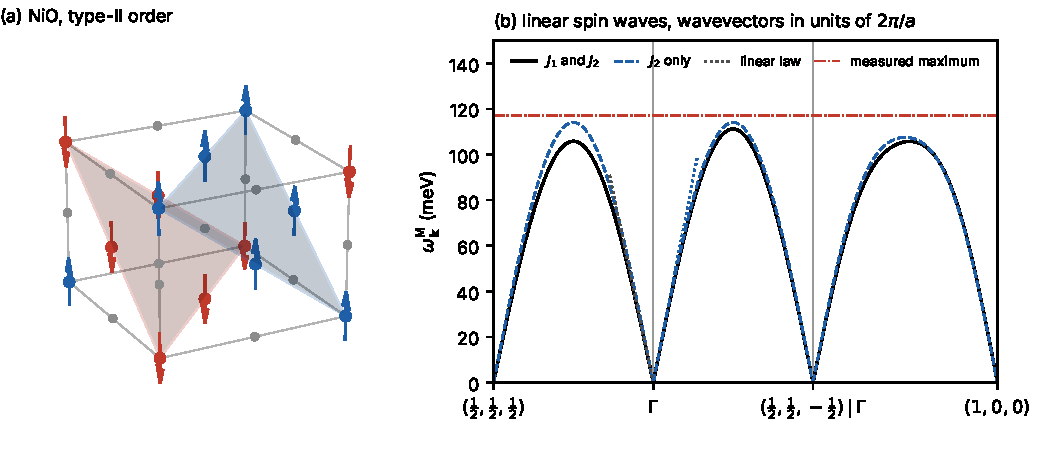
\includegraphics[width=\linewidth]{figures/ch07/fig7_1.pdf}
  \caption{Magnetic order and spin waves of NiO. (a) Conventional cubic cell of the rock-salt structure: nickel ions (colored) on the fcc sites, oxygen ions (gray) between them. In the type-II order the spins of each $(111)$ plane are parallel and alternate in sign from plane to plane; two of these planes are shaded. The arrows show only the sign of each moment; in NiO the moments lie within the planes, along a direction set by the weak anisotropy. (b) Magnon energies $\omega^{\mathrm{M}}_{\vect{k}}$ (meV) from linear spin-wave theory, \cref{eq:7.1-afm}, along three lines from the zone center $\Gamma$, with wavevectors in units of $2\pi/a$ and $a = \SI{4.17}{\angstrom}$. Model: undistorted fcc lattice, Heisenberg exchange with $J_1 = -\SI{1.37}{meV}$ and $J_2 = \SI{19.01}{meV}$ (each pair counted once, positive antiferromagnetic) measured by neutron scattering, $|\vect{S}| = 1$, no anisotropy. Solid: $J_1$ and $J_2$; dashed: $J_2$ alone, \cref{eq:7.1-J2}. Dotted: the linear laws $2\sqrt3(J_1 + J_2)|\vect{S}|ak$ along $[111]$, and $2\sqrt3J_2|\vect{S}|ak$ for $J_2$ alone. Dash-dotted: the measured maximum, ${\sim}\SI{117}{meV}$. The point $(\frac12,\frac12,\frac12)$, along the stacking direction of the planes, is equivalent to $\Gamma$ in the magnetic structure, and the energy returns to zero there. The zeros at $(\frac12,\frac12,-\frac12)$ and $(1,0,0)$ are soft points of the undistorted model; in real NiO the small rhombohedral distortion lifts them to a few meV. The largest energy in the zone, $|\vect{S}|(6J_2 - 3J_1) = \SI{118.2}{meV}$, lies off these lines.}
  \label{fig:7-nio}
\end{figure}

\begin{workedexample}{The magnon velocity of NiO}\label{we:7-nio}
With the exchange constants \cref{eq:7.1-NiO}, $|\vect{S}| = 1$ for Ni$^{2+}$, and the measured lattice constant $a = \SI{4.17}{\angstrom}$ as tabulated by Fischer et al.~\cite[Table~I]{fischer2009exchange}, \cref{eq:7.1-J2} gives the magnon velocity for $J_2$ alone
\begin{equation*}
  2\sqrt3\,J_2|\vect{S}|\,a = 2\sqrt3\times\SI{19.01}{meV}\times\SI{4.17}{\angstrom} = \SI{274.6}{meV.\angstrom} .
\end{equation*}
Dividing by $\hbar c = \SI{1973.27}{eV.\angstrom}$ turns this velocity into $1.39\times10^{-4}$ in natural units, or \SI{41.7}{km/s}. The nearest-neighbor exchange modifies the velocity. Along $[111]$, the direction normal to the ferromagnetic planes, the 6 parallel neighbors lie in a plane perpendicular to $\vect{k}$ and drop out of \cref{eq:D.19-linear}. Each of the 6 antiparallel ones has $(\vect{k}\cdot\vect{\delta})^2 = a^2k^2/3$, the same as each next-nearest neighbor contributes on average, and $J^{\mathrm{ex}}_{\mathrm{AB}}(0) = 6(J_1 + J_2)$. The bracket of \cref{eq:D.19-linear} is $2a^2k^2(J_1 + J_2)$, and
\begin{equation*}
  \omega^{\mathrm{M}}_{\vect{k}} \simeq 2\sqrt3\,(J_1 + J_2)|\vect{S}|\,ak = \SI{254.8}{meV.\angstrom}\times k \qquad (\vect{k} \parallel [111]) .
\end{equation*}
In other directions the parallel bonds no longer drop out, and evaluating \cref{eq:7.1-afm} numerically at small $k$ gives slopes between 255 and \SI{269}{meV.\angstrom}. The measured initial slope is ${\sim}\SI{250}{meV.\angstrom}$.

The largest magnon energy follows from a bound. With $J_1 < 0$, the in-plane sum $J^{\mathrm{ex}}_{\mathrm{AA}}(\vect{k}) = J_1\sum_{\vect{\delta}}\cos\vect{k}\cdot\vect{\delta}$ over the 6 parallel neighbors is largest when the cosines sum to their minimum, $-3$, the value of a triangular lattice at the corner of its zone. Then $A_{\vect{k}} \le J^{\mathrm{ex}}_{\mathrm{AB}}(0) - J^{\mathrm{ex}}_{\mathrm{AA}}(0) - 3J_1 = 6J_2 - 3J_1$, and $\omega^{\mathrm{M}}_{\vect{k}} \le |\vect{S}|A_{\vect{k}}$ with equality where $B_{\vect{k}} = 0$. The cosine minimum and the condition $B_{\vect{k}} = 0$ hold at the same $\vect{k}$, where $\omega^{\mathrm{M}}_{\mathrm{max}} = |\vect{S}|(6J_2 - 3J_1) = \SI{118.2}{meV}$, against $6J_2|\vect{S}| = \SI{114.1}{meV}$ for $J_2$ alone and a measured maximum of ${\sim}\SI{117}{meV}$. Linear spin-wave theory with two exchange constants thus reproduces both ends of the measured spectrum to a few percent. The agreement is partly by construction, since the exchange constants were fitted to the same data, and it does not test the $1/|\vect{S}|$ corrections, which a fit absorbs into $J_1$ and $J_2$.

The magnon velocity, $1.39\times10^{-4}$, is 19 times smaller than the fastest dark-matter speed in the laboratory, $v_{\mathrm{max}} = 2.650\times10^{-3}$ (\cref{sec:1.3}), and five times larger than the longitudinal sound speed of silicon, \SI{8.43}{km/s} along $[100]$ (\cref{app:C.18}). A dark-matter particle moves faster than the magnons it can emit. Emitting a magnon near the zone center is kinematically allowed in the same way as emitting an acoustic phonon, and at the same momentum transfer magnon emission deposits about five times more energy than phonon emission.
\end{workedexample}

\subsection{Spin-density response}

A probe that couples to the spin of the electron, such as a slow neutron or a dark-matter particle with a spin-dependent interaction, couples to the \emph{electron spin density}
\begin{equation}
  \vect{s}_e(\vect{q}) = \sum_i\ee^{\ii\vect{q}\cdot\vect{r}_i}\,\frac{\vect{\sigma}_i}{2} ,
  \label{eq:7.1-se}
\end{equation}
the spin analog of the density $n_e(\vect{q})$ of \cref{sec:2.3}, with the Pauli matrices $\vect{\sigma}_i$ of electron $i$. Like $n_e(\vect{q})$, the spin density $\vect{s}_e(\vect{q})$ adds the momentum $\vect{q}$ to the target. For dark matter of spin $\frac12$ with a spin-dependent coupling, the interaction takes the form $-\sum_a\hat O_{\chi a}(\vect{q})\,s_{e,a}(\vect{q})$~\cite[Eq.~(4)]{trickle2020detecting}, with an operator $\hat O_{\chi a}$ that acts on the spin of the dark-matter particle; \cref{sec:8.1} lists and derives these operators. The three components $s_{e,a}(\vect{q})$ are then target operators $O_a$ of the response matrix $S_{ab}$ of \cref{eq:4.2-Sab}, as the density was for a charge coupling.

In a magnetic insulator the spin density is localized on the ions. The filled shells carry no spin, and the unpaired electrons of ion $j$ occupy an open shell whose spin, at low energy, is $\vect{S}_j$. Within the ground multiplet of the ion every vector operator is proportional to $\vect{S}_j$, by the Wigner--Eckart theorem: the matrix elements of any vector operator within a multiplet of fixed total spin are those of the spin itself times one constant. The spin density near ion $j$ is therefore $\vect{S}_j\,\varrho_{\mathrm{s}}(\vect{r} - \vect{R}_j)$, with $\varrho_{\mathrm{s}}$ the normalized density of the unpaired electrons. The Fourier transform of the spin density is
\begin{equation}
  \vect{s}_e(\vect{q}) = F^{\mathrm{mag}}(q)\sum_j\ee^{\ii\vect{q}\cdot\vect{R}_j}\,\vect{S}_j, \qquad
  F^{\mathrm{mag}}(q) = \int\dd^3r\,\ee^{\ii\vect{q}\cdot\vect{r}}\,\varrho_{\mathrm{s}}(\vect{r}) ,
  \label{eq:7.1-Fmag}
\end{equation}
where $F^{\mathrm{mag}}(q)$, the \emph{magnetic form factor} of the ion, is spherically averaged and normalized to $F^{\mathrm{mag}}(0) = 1$. It is the spin analog of the atomic form factor of \cref{sec:2.2}. For a $3d$ shell it stays close to one up to the inverse shell radius, a few \si{\angstrom^{-1}} or several keV (\cref{app:C.19}), above most momentum transfers of sub-MeV dark matter. \Cref{app:C.19} adds the orbital moment of shells that have one and derives the neutron cross-section, which measures the same $S_{ab}$. \Cref{eq:7.1-Fmag} reduces the response of the electrons to the response of the ionic spins, a quantity that linear spin-wave theory supplies.

For the ferromagnet, at zero temperature, the transverse spin operators create single magnons. Define $S^\pm(\vect{q}) = \sum_j\ee^{\ii\vect{q}\cdot\vect{R}_j}S^\pm_j$. At linear order $S^-_j \simeq (2|\vect{S}|)^{1/2}d^\dagger_j$, and with $d^\dagger_j = N^{-1/2}\sum_{\vect{k}}\ee^{-\ii\vect{k}\cdot\vect{R}_j}a^\dagger_{\vect{k}}$ and the lattice sum \cref{eq:3.1-latticesum},
\begin{equation*}
  S^-(\vect{q}) \simeq (2|\vect{S}|N)^{1/2}\,a^\dagger_{\vect{q}_r} ,
\end{equation*}
where $\vect{q} = \vect{q}_r + \vect{G}_{\vect{q}}$ is the split of \cref{eq:3.1-qsplit} into a wavevector in the zone and a reciprocal-lattice vector. Crystal momentum is conserved: the magnon carries $\vect{q}_r$, and the lattice takes $\vect{G}_{\vect{q}}$. The operator $S^+(\vect{q})$ annihilates the ground state, which is fully polarized, and $S^z$ is quadratic in the bosons and creates no single magnon. With $s_{e,x} = F^{\mathrm{mag}}(S^+ + S^-)/2$ and $s_{e,y} = F^{\mathrm{mag}}(S^+ - S^-)/2\ii$, the one-magnon matrix elements are $\langle\vect{q}_r|s_{e,x}|0\rangle = F^{\mathrm{mag}}(2|\vect{S}|N)^{1/2}/2$ and $\langle\vect{q}_r|s_{e,y}|0\rangle = \ii F^{\mathrm{mag}}(2|\vect{S}|N)^{1/2}/2$. Inserting them into \cref{eq:4.2-Sab} with $\Vol = N\Omega$, where $\Omega$ is the volume per magnetic ion, gives:
\begin{keyresult}[One-magnon spin response of a ferromagnet]
\begin{equation}
  S_{ab}(\vect{q},\omega) = \frac{\pi|\vect{S}|}{\Omega}\,|F^{\mathrm{mag}}(q)|^2\,\bigl(\delta_{ab} - \hat z_a\hat z_b + \ii\epsilon_{abc}\hat z_c\bigr)\,\delta\bigl(\omega - \omega^{\mathrm{M}}_{\vect{q}_r}\bigr) ,
  \label{eq:7.1-Sfm}
\end{equation}
for $T = 0$, $\omega > 0$, and spins ordered along $\hat{\vect{z}}$, with $a, b$ the Cartesian components of $\vect{s}_e$.
\end{keyresult}
The matrix in brackets has the eigenvalues 2, for the circular combination $s_{e,x} - \ii s_{e,y}$ that lowers the spin, and 0 for the other two: \cref{eq:7.1-Sfm} is Hermitian and positive semidefinite, as \cref{eq:4.2-positivity} requires. A ferromagnet absorbs only the sense of rotation in which its spins precess, and this sense of rotation is the polarization vector $(|\vect{S}|/2)^{1/2}(1, \ii, 0)$ of Ref.~\cite[Eq.~(6)]{trickle2020detecting}. Apart from $|F^{\mathrm{mag}}|^2$ the one-magnon weight does not depend on $\vect{q}$. Through the fluctuation--dissipation theorem \cref{eq:4.2-fdt}, the same delta function is a pole of the transverse spin response $R_{ab}$, the susceptibility that magnetic resonance and neutron scattering measure.

In the antiferromagnet a transverse spin operator again creates one magnon, now with the amplitudes of \cref{eq:7.1-bogo}. The part of $S^+(\vect{k})$ on A is to linear order $S^+_{\mathrm{A}}(\vect{k}) \equiv \sum_{i\in\mathrm{A}}\ee^{\ii\vect{k}\cdot\vect{R}_i}S^+_i = (2|\vect{S}|N_{\mathrm{s}})^{1/2}d_{\mathrm{A},-\vect{k}}$, by the lattice sum $\sum_i\ee^{\ii(\vect{k}+\vect{k}')\cdot\vect{R}_i} = N_{\mathrm{s}}\delta_{\vect{k},-\vect{k}'}$. Inverting \cref{eq:7.1-bogo} as in \cref{app:C.7} gives
\begin{equation}
  d_{\mathrm{A}\vect{k}} = u^{\mathrm{M}}_{\vect{k}}\,a_{\vect{k}1} - v^{\mathrm{M}}_{\vect{k}}\,a^\dagger_{\vect{k}2}, \qquad
  d_{\mathrm{B}\vect{k}} = u^{\mathrm{M}}_{\vect{k}}\,a_{\vect{k}2} - v^{\mathrm{M}}_{\vect{k}}\,a^\dagger_{\vect{k}1} .
  \label{eq:D.19-inverse}
\end{equation}
On B the raising operator is $S^+_j \simeq (2|\vect{S}|)^{1/2}d^\dagger_{\mathrm{B}j}$, and the same lattice sum turns $\sum_{j\in\mathrm{B}}\ee^{\ii\vect{k}\cdot\vect{R}_j}d^\dagger_{\mathrm{B}j}$ into $N_{\mathrm{s}}^{1/2}d^\dagger_{\mathrm{B},-\vect{k}}$. Since $A_{\vect{k}}$ and $B_{\vect{k}}$, and with them $u^{\mathrm{M}}_{\vect{k}}$ and $v^{\mathrm{M}}_{\vect{k}}$, are even in $\vect{k}$, the sum of the contributions of both sublattices at small $\vect{k}$ is $S^+(\vect{k}) \simeq (2|\vect{S}|N_{\mathrm{s}})^{1/2}(d_{\mathrm{A},-\vect{k}} + d^\dagger_{\mathrm{B},-\vect{k}}) = (2|\vect{S}|N_{\mathrm{s}})^{1/2}(u^{\mathrm{M}}_{\vect{k}} - v^{\mathrm{M}}_{\vect{k}})(a_{-\vect{k}1} + a^\dagger_{-\vect{k}2})$. Near the ordering wavevector, where the two sublattices enter with opposite phases, the one-magnon amplitude is $(2|\vect{S}|N_{\mathrm{s}})^{1/2}(u^{\mathrm{M}}_{\vect{k}} + v^{\mathrm{M}}_{\vect{k}})$. From the expressions of $\cosh2\theta_{\vect{k}}$ and $\sinh2\theta_{\vect{k}}$ in \cref{app:C.7},
\begin{equation}
  \bigl(u^{\mathrm{M}}_{\vect{k}} \mp v^{\mathrm{M}}_{\vect{k}}\bigr)^2 = \frac{A_{\vect{k}} \mp B_{\vect{k}}}{(A_{\vect{k}}^2 - B_{\vect{k}}^2)^{1/2}} = \frac{|\vect{S}|(A_{\vect{k}} \mp B_{\vect{k}})}{\omega^{\mathrm{M}}_{\vect{k}}} .
  \label{eq:7.1-weights}
\end{equation}
Near $\Gamma$, $A_{\vect{k}} - B_{\vect{k}} \propto k^2$ while $\omega^{\mathrm{M}}_{\vect{k}} \propto k$, so the weight near $\Gamma$ vanishes linearly in $k$: a uniform field cannot tilt two opposite sublattices without working against the exchange field. Near the ordering wavevector the weight grows as the inverse distance from that wavevector. Unlike the ferromagnet, the antiferromagnet thus distributes its one-magnon weight unevenly: at the same $\vect{k}$ the weights near $\Gamma$ and near the ordering wavevector differ by the factor $(A_{\vect{k}} + B_{\vect{k}})/(A_{\vect{k}} - B_{\vect{k}})$. Dark matter samples the suppressed weight near $\Gamma$ unless its momentum transfer reaches the ordering wavevector, $(\pi/a)(1,1,1)$ in NiO, of length $\sqrt3\pi/a = \SI{1.30}{\angstrom^{-1}} = \SI{2.6}{keV}$. Since $q \le 2\mchi v_{\mathrm{max}}$, reaching the ordering wavevector takes $\mchi \gtrsim \SI{0.5}{MeV}$. The longitudinal component $S^z$ creates magnons in pairs.

\section{Superconductivity}\label{sec:7.2}

Aluminum loses its electrical resistance below \SI{1.18}{K}, and at the lowest temperatures tunneling measures an energy gap of \SI{0.18}{meV} at its Fermi surface~\cite[Table~III]{savrasov1996electron}. Unlike a band gap, it opens because the electrons within a few tens of meV of the Fermi surface bind into pairs, and an excitation that conserves the number of electrons must break a pair, at a cost of $2\Delta_{\mathrm{BCS}} \approx \SI{0.36}{meV}$. This is the smallest quantum of \cref{tab:1-quanta}, and by the bound $m_{\mathrm{min}} = 2E_{\mathrm{th}}/v_{\mathrm{max}}^2$ of \cref{sec:1.3} it would let dark matter far below a keV deposit detectable energy (\cref{we:7-al})~\cite{hochberg2016detecting}. Superconducting films are also the sensors that read out most phonon-based detectors (\cref{sec:1.5}). Where does the attraction that binds the pairs come from, and how strong is it? What are the excitations of the paired state, and how do the density and the spin density of the electrons create them? And does the answer respect charge conservation, which the simplest treatment of the paired state does not? We start from the electron--phonon vertex of \cref{sec:6.2}.

\subsection{The phonon-mediated attraction}

Two electrons repel each other through the Coulomb interaction, yet in a metal they can attract each other by exchanging a phonon. \Cref{app:D.11} showed how. In the diagram rules, a phonon line replaces the Coulomb line, and with the normalization of \cref{eq:A.6-Hep}, in which the vertex $g$ comes with $1/\sqrt N$, the rule \cref{eq:D.11-boson} reads $-v_{\mathrm{C}}/\Vol \to -|g|^2\mathsf{D}_0(\vect{Q},\omega)/N$. Two electrons that exchange energy $\omega$ through a phonon $(\vect{Q},\nu)$ therefore feel the interaction
\begin{equation}
  \frac{1}{N}\,|g_\nu(\vect{k},\vect{Q})|^2\,\mathsf{D}_0(\vect{Q}\nu,\omega) = \frac{1}{N}\,\frac{2\omega_{\vect{Q}\nu}\,|g_\nu(\vect{k},\vect{Q})|^2}{\omega^2 - \omega_{\vect{Q}\nu}^2} ,
  \label{eq:7.2-Veff}
\end{equation}
with $g_\nu$ the vertex of a single band at the Fermi level, whose band indices we drop. For $|\omega| < \omega_{\vect{Q}\nu}$ it is negative, an attraction. The attraction is retarded. An electron moving through the crystal pulls the ions toward its path, and the ions, which respond on the scale $1/\omega_{\vect{Q}\nu}$, are still displaced after the electron has left. A second electron that arrives within that time is attracted by the positive charge the first one left behind. The screened Coulomb repulsion between the two acts only when they are close at the same moment, and by then the first electron is far away. Bardeen and Pines combined the two interactions in the electron gas and found the net interaction attractive for energy transfers below the phonon energy~\cite{bardeen1955electron}. In a scattering of two electrons near the Fermi surface the energy transfer is $\omega = \xi_{\vect{k}'} - \xi_{\vect{k}}$, with $\xi_{\vect{k}}$ the band energy measured from the Fermi level. The attraction acts between electrons whose energies lie within about the Debye frequency $\omega_{\mathrm{D}}$ of the Fermi surface, the scale of the largest phonon energies (\cref{sec:5.2}).

\paragraph{The pairing strength.} Take two electrons of opposite momentum and spin, $(\vect{k}\!\uparrow, -\vect{k}\!\downarrow)$, and let them scatter into $(\vect{k}'\!\uparrow, -\vect{k}'\!\downarrow)$ with $\vect{Q} = \vect{k}' - \vect{k}$. For energy transfers small compared with the phonon energy, \cref{eq:7.2-Veff} is its static value $-2|g_\nu|^2/(N\omega_{\vect{Q}\nu})$. In the interaction Hamiltonian $(1/2N)\sum_{\vect{Q}}v(\vect{Q})\,n_e(\vect{Q})n_e(-\vect{Q})$ the pair process appears twice, once with the spin-up electron in $n_e(\vect{Q})$ and once with the spin-down electron there, which cancels the $\frac12$. Time reversal makes the vertex of the spin-down electron, $g_\nu(-\vect{k},-\vect{Q})$, the complex conjugate of $g_\nu(\vect{k},\vect{Q})$, so the product of the two vertices is $|g_\nu(\vect{k},\vect{Q})|^2$. The pair term is therefore
\begin{equation*}
  -\frac{2}{N}\sum_\nu\frac{|g_\nu(\vect{k},\vect{Q})|^2}{\omega_{\vect{Q}\nu}}\;c^\dagger_{\vect{k}'\uparrow}c^\dagger_{-\vect{k}'\downarrow}c_{-\vect{k}\downarrow}c_{\vect{k}\uparrow} .
\end{equation*}
The model of Bardeen, Cooper and Schrieffer~\cite{bardeen1957theory} replaces the coefficient by a constant $-V_{\mathrm{BCS}}/\Vol$, with $\Vol = N\Omega$ the volume of the crystal and $\Omega$ the unit-cell volume, for all $\vect{k}$ and $\vect{k}'$ within $\omega_{\mathrm{D}}$ of the Fermi surface, and by zero outside that shell. The natural constant is the Fermi-surface average, $V_{\mathrm{BCS}} = 2\Omega\langle\sum_\nu|g_\nu|^2/\omega_{\vect{Q}\nu}\rangle_{\mathrm{FS}}$, where $\langle X\rangle_{\mathrm{FS}} = \sum_{\vect{k}\vect{k}'}X\,\delta(\xi_{\vect{k}})\delta(\xi_{\vect{k}'})/[\sum_{\vect{k}}\delta(\xi_{\vect{k}})]^2$ averages over both electrons on the Fermi surface. With $\sum_{\vect{k}}\delta(\xi_{\vect{k}}) = N\Omega\,\mathcal{N}_{\mathrm{F}}$ for one spin orientation and the Eliashberg function \cref{eq:6.4-a2F},
\begin{equation*}
  \mathcal{N}_{\mathrm{F}}V_{\mathrm{BCS}} = \frac{2}{\mathcal{N}_{\mathrm{F}}\Omega\,N^2}\sum_{\vect{k}\vect{Q}\nu}\frac{|g_\nu(\vect{k},\vect{Q})|^2}{\omega_{\vect{Q}\nu}}\,\delta(\xi_{\vect{k}})\,\delta(\xi_{\vect{k}+\vect{Q}}) = 2\int_0^\infty\dd\omega\,\frac{\alpha^2F(\omega)}{\omega} .
\end{equation*}
The right side is the coupling constant of \cref{eq:6.4-lambda}:
\begin{keyresult}[Phonon-mediated pairing strength]
\begin{equation}
  \mathcal{N}_{\mathrm{F}}V_{\mathrm{BCS}} = \lambda_{\mathrm{ep}} .
  \label{eq:7.2-NV}
\end{equation}
\end{keyresult}
The dimensionless strength of the attraction is the same number that enhances the electron mass and that the phonon linewidths of \cref{sec:6.4} measure.

\Cref{eq:7.2-NV} leaves out the Coulomb repulsion and the quasiparticle renormalization, both of the same order. The screened Coulomb repulsion acts at all energy transfers, while the attraction acts only within $\omega_{\mathrm{D}}$ of the Fermi surface. Its Fermi-surface average is reduced by this mismatch of time scales to the Coulomb pseudopotential $\mu^*_{\mathrm{C}}$ of \cref{app:E.9}, of order 0.1, which subtracts from $\lambda_{\mathrm{ep}}$. The pairing electrons are, in addition, the quasiparticles of \cref{sec:6.4}, with the residue $1/(1 + \lambda_{\mathrm{ep}})$. The Eliashberg equations contain both effects. At low frequencies the renormalization function of \cref{eq:E.9-Z} is $1 + \lambda_{\mathrm{ep}}$, the mass enhancement. If we go further and cut the frequency-dependent coupling \cref{eq:E.9-lambda} off at about $\omega_{\mathrm{D}}$, replacing it by $\lambda_{\mathrm{ep}}$ below and by zero above, the Eliashberg gap equation \cref{eq:E.9-Delta} reduces to the BCS one derived below, \cref{eq:7.2-gap}, written in Matsubara form, with the effective coupling
\begin{equation}
  \mathcal{N}_{\mathrm{F}}V_{\mathrm{BCS}} \simeq \frac{\lambda_{\mathrm{ep}} - \mu^*_{\mathrm{C}}}{1 + \lambda_{\mathrm{ep}}} .
  \label{eq:7.2-NVren}
\end{equation}
For aluminum, with $\lambda_{\mathrm{ep}} = 0.44$ and $\mu^*_{\mathrm{C}} = 0.12$, this is 0.22, half of \cref{eq:7.2-NV}. In practice the gap of a real superconductor is computed by solving the Eliashberg equations with the $\alpha^2F$ of \cref{sec:6.4}, which comes from density-functional perturbation theory and Wannier interpolation.

\paragraph{The reduced Hamiltonian.} The attraction scatters pairs of any total momentum, but pairs of zero total momentum have the most final states. For every $\vect{k}$ in the shell, every $\vect{k}'$ in the shell is a possible final state of the pair $(\vect{k}\!\uparrow, -\vect{k}\!\downarrow)$. A pair with total momentum $\vect{P} \ne 0$, by contrast, needs both $\vect{k}$ and $\vect{P} - \vect{k}$ in the shell, a condition that removes most of the phase space once $|\vect{P}|$ exceeds $\omega_{\mathrm{D}}/v_{\mathrm{F}}$. The \emph{reduced} BCS Hamiltonian keeps only the zero-momentum pairs:
\begin{equation}
  H_{\mathrm{BCS}} = \sum_{\vect{k}\sigma}\xi_{\vect{k}}\,c^\dagger_{\vect{k}\sigma}c_{\vect{k}\sigma} - \frac{V_{\mathrm{BCS}}}{\Vol}{\sum_{\vect{k}\vect{k}'}}'c^\dagger_{\vect{k}\uparrow}c^\dagger_{-\vect{k}\downarrow}c_{-\vect{k}'\downarrow}c_{\vect{k}'\uparrow} ,
  \label{eq:7.2-HBCS}
\end{equation}
with the prime restricting $|\xi_{\vect{k}}|$ and $|\xi_{\vect{k}'}|$ to less than $\omega_{\mathrm{D}}$. The pairs of finite momentum return when we ask how the paired state responds to a probe at wavevector $\vect{q}$.

\subsection{Cooper pairs and the BCS state}

\paragraph{Mean field.} The paired state follows from the mean-field theory of \cref{app:D.20}. Define the pair amplitude $b_{\vect{k}} = \langle c_{-\vect{k}\downarrow}c_{\vect{k}\uparrow}\rangle$, which is zero in any state with a definite number of electrons, and the gap
\begin{equation}
  \Delta_{\mathrm{BCS}} = \frac{V_{\mathrm{BCS}}}{\Vol}{\sum_{\vect{k}}}'b_{\vect{k}} ,
  \label{eq:7.2-Delta}
\end{equation}
real by the choice of an overall phase. In \cref{eq:7.2-HBCS} each pair operator interacts with all $\sim N$ others with a strength of order $1/\Vol$, and replacing their sum by its average, \cref{eq:7.2-Delta}, makes an error that vanishes as $\Vol \to \infty$. The interaction then becomes the pair field $-\Delta_{\mathrm{BCS}}(c^\dagger_{\vect{k}\uparrow}c^\dagger_{-\vect{k}\downarrow} + c_{-\vect{k}\downarrow}c_{\vect{k}\uparrow})$ acting on each pair of modes, and for each $\vect{k}$ the mean-field Hamiltonian $H_{\mathrm{MF}}$ is the two-mode fermion problem \cref{eq:C.7-Hfermion} with $\xi_0 = \xi_{\vect{k}}$ and $g_0 = \Delta_{\mathrm{BCS}}$. It is diagonalized by the fermionic Bogoliubov transformation of \cref{app:C.7}, the counterpart of the bosonic one that diagonalized the antiferromagnet in \cref{sec:7.1}, with sines and cosines in place of hyperbolic functions. The quasiparticle operators are
\begin{equation}
  \gamma_{\vect{k}1} = u^{\mathrm{B}}_{\vect{k}}\,c_{\vect{k}\uparrow} - v^{\mathrm{B}}_{\vect{k}}\,c^\dagger_{-\vect{k}\downarrow}, \qquad
  \gamma_{\vect{k}2} = u^{\mathrm{B}}_{\vect{k}}\,c_{-\vect{k}\downarrow} + v^{\mathrm{B}}_{\vect{k}}\,c^\dagger_{\vect{k}\uparrow} ,
  \label{eq:7.2-gamma}
\end{equation}
and by \cref{eq:C.7-Efermion},
\begin{keyresult}[Bogoliubov quasiparticles]
\begin{equation}
  \begin{gathered}
  H_{\mathrm{MF}} = {\sum_{\vect{k}}}'E_{\vect{k}}\bigl(\gamma^\dagger_{\vect{k}1}\gamma_{\vect{k}1} + \gamma^\dagger_{\vect{k}2}\gamma_{\vect{k}2}\bigr) + \text{const}, \qquad
  E_{\vect{k}} = \bigl(\xi_{\vect{k}}^2 + \Delta_{\mathrm{BCS}}^2\bigr)^{1/2}, \\
  (u^{\mathrm{B}}_{\vect{k}})^2 = \frac12\Bigl(1 + \frac{\xi_{\vect{k}}}{E_{\vect{k}}}\Bigr), \qquad
  (v^{\mathrm{B}}_{\vect{k}})^2 = \frac12\Bigl(1 - \frac{\xi_{\vect{k}}}{E_{\vect{k}}}\Bigr), \qquad
  2u^{\mathrm{B}}_{\vect{k}}v^{\mathrm{B}}_{\vect{k}} = \frac{\Delta_{\mathrm{BCS}}}{E_{\vect{k}}} .
  \end{gathered}
  \label{eq:7.2-E}
\end{equation}
\end{keyresult}
The coefficients $u^{\mathrm{B}}_{\vect{k}}$ and $v^{\mathrm{B}}_{\vect{k}}$ are the \emph{coherence factors} of the BCS state. The quasiparticle $\gamma^\dagger_{\vect{k}1}$ carries momentum $\vect{k}$ and spin up. Far above the Fermi surface $u^{\mathrm{B}}_{\vect{k}} \to 1$ and it is an added electron; far below, $v^{\mathrm{B}}_{\vect{k}} \to 1$ and it is a removed electron of momentum $-\vect{k}$ and spin down, a hole; at the Fermi surface it is half of each, with energy $\Delta_{\mathrm{BCS}}$. The ground state, annihilated by every $\gamma$, is the BCS state
\begin{equation}
  |\mathrm{BCS}\rangle = \prod_{\vect{k}}\bigl(u^{\mathrm{B}}_{\vect{k}} + v^{\mathrm{B}}_{\vect{k}}\,c^\dagger_{\vect{k}\uparrow}c^\dagger_{-\vect{k}\downarrow}\bigr)|0\rangle ,
  \label{eq:7.2-BCS}
\end{equation}
in which each pair state $(\vect{k}\!\uparrow, -\vect{k}\!\downarrow)$ is occupied with probability $(v^{\mathrm{B}}_{\vect{k}})^2$. The step of the Fermi sea is smeared over an energy $\Delta_{\mathrm{BCS}}$, and the coherent superposition of empty and full pair states is what makes $b_{\vect{k}} = u^{\mathrm{B}}_{\vect{k}}v^{\mathrm{B}}_{\vect{k}}$ nonzero. The state $|\mathrm{BCS}\rangle$ has no definite electron number. Its relative number fluctuations are of order $N^{-1/2}$. They are negligible for energies but spoil the density response, which the last subsection repairs.

\paragraph{Quasiparticle density of states.} Since $\dd E_{\vect{k}}/\dd\xi_{\vect{k}} = \xi_{\vect{k}}/E_{\vect{k}}$, each energy $E > \Delta_{\mathrm{BCS}}$ is reached from two values of $\xi$, an electronlike state above the Fermi level and a holelike one below. With $\mathcal{N}_{\mathrm{F}}$ constant over the shell, the quasiparticles of one spin orientation have the density of states per volume
\begin{equation}
  \mathcal{N}_{\mathrm{qp}}(E) = 2\mathcal{N}_{\mathrm{F}}\,\frac{E}{\sqrt{E^2 - \Delta_{\mathrm{BCS}}^2}}\,\Theta(E - \Delta_{\mathrm{BCS}}) .
  \label{eq:7.2-dos}
\end{equation}
The factor 2 counts the two branches, not the spin; both spin orientations together have $g_{\mathrm{deg}}\mathcal{N}_{\mathrm{qp}}$, with $g_{\mathrm{deg}} = 2$. In the normal metal, $\mathcal{N}_{\mathrm{qp}} \to 2\mathcal{N}_{\mathrm{F}}$, the density of electron and hole excitations at energy $E$ above the ground state. Pairing removes the states from $|E| < \Delta_{\mathrm{BCS}}$ and piles them up at the edge, where the density diverges as $(E - \Delta_{\mathrm{BCS}})^{-1/2}$ (\cref{fig:7-bcs}a). The number of states is conserved: $\int_{\Delta_{\mathrm{BCS}}}^{\omega}\dd E\,\mathcal{N}_{\mathrm{qp}} = 2\mathcal{N}_{\mathrm{F}}(\omega^2 - \Delta_{\mathrm{BCS}}^2)^{1/2}$, which approaches the normal-state count $2\mathcal{N}_{\mathrm{F}}\omega$ as $\omega$ grows.

\paragraph{The gap equation.} The gap must reproduce itself through \cref{eq:7.2-Delta}. In thermal equilibrium the quasiparticles are independent fermions, occupied with $n_{\mathrm{F}}(E_{\vect{k}})$, and inverting \cref{eq:7.2-gamma} yields $b_{\vect{k}} = u^{\mathrm{B}}_{\vect{k}}v^{\mathrm{B}}_{\vect{k}}[1 - 2n_{\mathrm{F}}(E_{\vect{k}})] = (\Delta_{\mathrm{BCS}}/2E_{\vect{k}})\tanh(E_{\vect{k}}/2T)$. Inserting this, dividing by $\Delta_{\mathrm{BCS}}$ and replacing $\Vol^{-1}\sum_{\vect{k}}$ by $\mathcal{N}_{\mathrm{F}}\int\dd\xi$,
\begin{keyresult}[BCS gap equation and its weak-coupling solutions]
\begin{equation}
  \begin{gathered}
  \frac{1}{\mathcal{N}_{\mathrm{F}}V_{\mathrm{BCS}}} = \int_0^{\omega_{\mathrm{D}}}\dd\xi\,\frac{\tanh\bigl(\sqrt{\xi^2 + \Delta_{\mathrm{BCS}}^2}/2T\bigr)}{\sqrt{\xi^2 + \Delta_{\mathrm{BCS}}^2}} , \\
  \Delta_{\mathrm{BCS}}(0) \simeq 2\omega_{\mathrm{D}}\,\ee^{-1/\mathcal{N}_{\mathrm{F}}V_{\mathrm{BCS}}}, \qquad
  T_c = \frac{2\ee^{\gamma_{\mathrm{E}}}}{\pi}\,\omega_{\mathrm{D}}\,\ee^{-1/\mathcal{N}_{\mathrm{F}}V_{\mathrm{BCS}}}, \\
  \frac{\Delta_{\mathrm{BCS}}(0)}{T_c} = \pi\ee^{-\gamma_{\mathrm{E}}} = 1.764 ,
  \end{gathered}
  \label{eq:7.2-gap}
\end{equation}
\end{keyresult}
with $\gamma_{\mathrm{E}} = 0.5772$ Euler's constant. The right side of the gap equation diverges logarithmically as $\Delta_{\mathrm{BCS}}$ and $T$ go to zero, which is why a solution exists for any attraction. A weak attraction does not bind two particles in three-dimensional vacuum, where the density of pair states vanishes as $\xi^{1/2}$ and the integral converges; above a Fermi surface that density stays finite down to zero energy. At $T = 0$ the integral is $\operatorname{arsinh}(\omega_{\mathrm{D}}/\Delta_{\mathrm{BCS}})$, and the gap follows; at $T_c$ the gap closes, and the integral, evaluated in \cref{app:D.20} by expanding the hyperbolic tangent over Matsubara frequencies, fixes the critical temperature. The gap is nonanalytic in the coupling and invisible at any finite order of perturbation theory. Both $\Delta_{\mathrm{BCS}}(0)$ and $T_c$ depend exponentially on $\mathcal{N}_{\mathrm{F}}V_{\mathrm{BCS}}$ and linearly on the cutoff, but their ratio depends on neither, and it is the same for every material within the model. Deviations from 1.764 measure the strength and the retardation of the real interaction. Aluminum, with the measured \SI{0.18}{meV} and \SI{1.18}{K}, has $2\Delta_{\mathrm{BCS}}/T_c = 3.54$, against $2\pi\ee^{-\gamma_{\mathrm{E}}} = 3.53$.

\paragraph{The pair-breaking threshold.} A dark-matter particle or a phonon couples to the electrons through operators that conserve their number, such as the density $n_e(\vect{q})$ and the spin density. Expressed through \cref{eq:7.2-gamma}, such an operator either scatters a quasiparticle that is already present or creates two at once, one from each branch; it never creates a single one, which would change the electron number by one. At $T = 0$ no quasiparticles are present, and the lowest excitation that a probe can make is a pair, at
\begin{equation}
  \omega \ge E_{\vect{k}} + E_{\vect{k}+\vect{q}} \ge 2\Delta_{\mathrm{BCS}} ,
  \label{eq:7.2-threshold}
\end{equation}
the \emph{pair-breaking threshold}. It is reached when both quasiparticles lie at the Fermi surface, which for $q < 2k_{\mathrm{F}}$ is always possible. In the language of \cref{sec:1.3}, $E_{\mathrm{th}} = 2\Delta_{\mathrm{BCS}}$. At $T > 0$ thermally excited quasiparticles can absorb energy in smaller amounts, but their number is suppressed by $\ee^{-\Delta_{\mathrm{BCS}}/T}$, and in aluminum at \SI{10}{mK} the exponent is $-208$.

\begin{figure}[t]
  \centering
  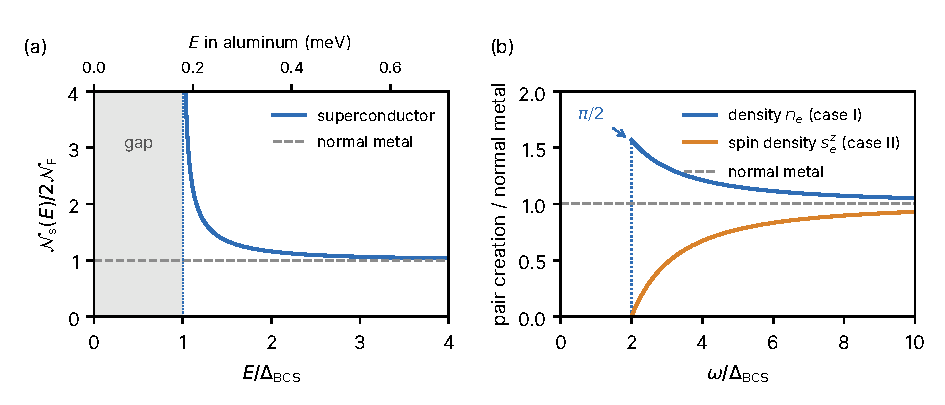
\includegraphics[width=\linewidth]{figures/ch07/fig7_2.pdf}
  \caption{Quasiparticles of a BCS superconductor at $T = 0$. (a) Density of states per spin orientation, \cref{eq:7.2-dos}, in units of its normal-state value $2\mathcal{N}_{\mathrm{F}}$: no states below $\Delta_{\mathrm{BCS}}$ (gray), an integrable divergence at the edge. The top axis shows the energy for aluminum, $\Delta_{\mathrm{BCS}} = 1.764\,T_c = \SI{0.179}{meV}$ with the measured $T_c = \SI{1.18}{K}$. (b) Rate of pair creation by a probe of energy $\omega$ coupled to the electron density (case I) or to the $z$ component of the spin density (case II), divided by its normal-state value, \cref{eq:7.2-pairspec}. Both are bare quasiparticle bubbles for a linearized band with $q \ll k_{\mathrm{F}}$ and $qv_{\mathrm{F}} \ge \omega$, the regime of dark-matter scattering in aluminum, where the ratio does not depend on $q$. The density curve jumps to $\pi/2$ at the threshold $2\Delta_{\mathrm{BCS}}$; the spin curve starts from zero and is the zero-temperature conductivity ratio of Mattis and Bardeen. Both tend to one for $\omega \gg \Delta_{\mathrm{BCS}}$.}
  \label{fig:7-bcs}
\end{figure}

\subsection{Coherence factors}

The amplitude to break a pair depends on what the probe couples to, because each quasiparticle is part electron and part hole and the two parts can interfere. Take the density, $n_e(\vect{q}) = \sum_{\vect{k}\sigma}c^\dagger_{\vect{k}+\vect{q},\sigma}c_{\vect{k}\sigma}$, and the $z$ component of the spin density of \cref{eq:7.1-se}, $s^z_e(\vect{q}) = \frac12\sum_{\vect{k}}(c^\dagger_{\vect{k}+\vect{q}\uparrow}c_{\vect{k}\uparrow} - c^\dagger_{\vect{k}+\vect{q}\downarrow}c_{\vect{k}\downarrow})$. Write $u = u^{\mathrm{B}}_{\vect{k}}$, $v = v^{\mathrm{B}}_{\vect{k}}$, and primes for $\vect{k}' = \vect{k} + \vect{q}$. Substituting the inverse of \cref{eq:7.2-gamma} into the spin-up term gives $c^\dagger_{\vect{k}'\uparrow}c_{\vect{k}\uparrow} = u'u\,\gamma^\dagger_{\vect{k}'1}\gamma_{\vect{k}1} + u'v\,\gamma^\dagger_{\vect{k}'1}\gamma^\dagger_{\vect{k}2} + \dots$, and the spin-down term, after relabeling $\vect{k} \to -\vect{k} - \vect{q}$, contributes to the same two processes with $-vv'$ and $uv'$ (\cref{app:D.20}). The density adds the spin-up and spin-down terms and the spin density subtracts them, so that the amplitudes are
\begin{equation}
  \begin{aligned}
  n_e(\vect{q}):&\quad \text{pair creation } u'v + v'u, \qquad \text{quasiparticle scattering } uu' - vv' ,\\
  s^z_e(\vect{q}):&\quad \text{pair creation } \tfrac12(u'v - v'u), \qquad \text{quasiparticle scattering } \tfrac12(uu' + vv') .
  \end{aligned}
  \label{eq:7.2-coh}
\end{equation}
Squared and expressed through the energies with \cref{eq:7.2-E},
\begin{keyresult}[Coherence factors of pair creation and quasiparticle scattering]
\begin{equation}
  (uv' \pm vu')^2 = \frac12\Bigl(1 - \frac{\xi\xi' \mp \Delta_{\mathrm{BCS}}^2}{EE'}\Bigr), \qquad
  (uu' \mp vv')^2 = \frac12\Bigl(1 + \frac{\xi\xi' \mp \Delta_{\mathrm{BCS}}^2}{EE'}\Bigr) ,
  \label{eq:7.2-cohE}
\end{equation}
\end{keyresult}
with the upper signs for the density and the lower signs for the spin density. The two operators differ in their behavior under time reversal: the density is even and the spin density odd. These are the two classes that Tinkham calls case~I and case~II~\cite{tinkham2004introduction}. Every one-body probe is a sum of a part even and a part odd under time reversal, one from each class; the current, which drives the absorption of light, is odd and belongs to case~II with the spin.

At the threshold both quasiparticles lie at the Fermi surface, $\xi = \xi' = 0$, and the creation factor is $\frac12(1 \pm 1)$: one for the density, zero for the spin density. In the density the electron and hole parts of the pair add; in the spin density they cancel. Away from the Fermi surface the factors depend on the signs of $\xi$ and $\xi'$, and the dark-matter kinematics decide how these are sampled. For a linearized band, $\xi' = \xi + v_{\mathrm{F}}q\cos\theta$ with $\theta$ the angle between $\vect{k}$ and $\vect{q}$. Two quasiparticles with $E + E' = \omega$ have $|\xi'- \xi| \le |\xi| + |\xi'| < \omega$, so as long as $v_{\mathrm{F}}q \ge \omega$ every pair of values $(\xi, \xi')$ in that range is reached at some angle. Since $\cos\theta$ is uniformly distributed over the Fermi sphere, each pair is reached with the same weight.

This is the regime of dark-matter scattering in a metal. A dark-matter particle that deposits $\omega$ transfers at least $q = \omega/v_{\mathrm{max}}$ (\cref{sec:1.3}), and in aluminum $v_{\mathrm{F}} = \num{6.75e-3}$, the free-electron value of \cref{sec:6.4}, is 2.5 times $v_{\mathrm{max}}$. Then $\xi$ and $\xi'$ are independent and uniformly distributed, and the terms odd in either one average to zero. The mean creation factor of the density becomes $\frac12(1 + \Delta_{\mathrm{BCS}}^2/EE')$, and that of the spin density $\frac12(1 - \Delta_{\mathrm{BCS}}^2/EE')$.

\paragraph{The pair-creation spectrum.} With these factors the absorption spectrum of the paired state follows in closed form. At $T = 0$ the dynamic structure factor of the density is the golden-rule sum over pairs, $S(\vect{q},\omega) = (2\pi/\Vol)\sum_{\vect{k}}(uv' + vu')^2\,\delta(\omega - E_{\vect{k}} - E_{\vect{k}+\vect{q}})$; the sum over $\vect{k}$ with both branches covers both spin orientations, as the normal limit below confirms. Replace $\Vol^{-1}\sum_{\vect{k}}$ by $\mathcal{N}_{\mathrm{F}}\int\dd\xi\int_{-1}^1\dd\!\cos\theta/2$, trade the angle for $\xi'$ at $\dd\xi'/2v_{\mathrm{F}}q$, and change variables from $\xi$ and $\xi'$ to $E$ and $E'$ with the density of states \cref{eq:7.2-dos} for each, which absorbs the sum over the four sign combinations. In the normal state, $\Delta_{\mathrm{BCS}} = 0$, the result is $S_{\mathrm{n}}(\vect{q},\omega) = 2\pi\mathcal{N}_{\mathrm{F}}\,\omega/v_{\mathrm{F}}q = m_e^2\omega/\pi q$, the electron gas of \cref{sec:4.5} below its curve $\omega = qv_{\mathrm{F}} - q^2/2m_e$. In the superconductor,
\begin{keyresult}[Bare pair-creation spectra for $qv_{\mathrm{F}} \ge \omega$]
\begin{equation}
  \frac{S_{\mathrm{I,II}}(\vect{q},\omega)}{S_{\mathrm{n}}(\vect{q},\omega)} = \frac{1}{\omega}\int_{\Delta_{\mathrm{BCS}}}^{\omega - \Delta_{\mathrm{BCS}}}\dd E\,\frac{E(\omega - E) \pm \Delta_{\mathrm{BCS}}^2}{\sqrt{E^2 - \Delta_{\mathrm{BCS}}^2}\,\sqrt{(\omega - E)^2 - \Delta_{\mathrm{BCS}}^2}}\;\Theta(\omega - 2\Delta_{\mathrm{BCS}}) ,
  \label{eq:7.2-pairspec}
\end{equation}
\end{keyresult}
with the upper sign for the density (case~I) and the lower sign for the spin density (case~II), each divided by its own normal-state value. \Cref{fig:7-bcs}(b) shows both. Near the threshold $E(\omega - E) \to \Delta_{\mathrm{BCS}}^2$, so the numerator of the integrand tends to $\Delta_{\mathrm{BCS}}^2 \pm \Delta_{\mathrm{BCS}}^2$, that is $2\Delta_{\mathrm{BCS}}^2$ for the density and zero for the spin density, while the denominator tends to $2\Delta_{\mathrm{BCS}}$ times the product of the two edge divergences of \cref{eq:7.2-dos}. The integral of that product over the shrinking interval stays finite, $\int\dd E\,[(E - \Delta_{\mathrm{BCS}})(\omega - \Delta_{\mathrm{BCS}} - E)]^{-1/2} = \pi$. For the density the integral is therefore $\Delta_{\mathrm{BCS}}\pi$, and with the prefactor $1/\omega = 1/2\Delta_{\mathrm{BCS}}$ the spectrum jumps at $\omega = 2\Delta_{\mathrm{BCS}}$ to $\pi/2$ times the normal value. Since $E(\omega - E) - \Delta^2_{\mathrm{BCS}}$ vanishes at the threshold, the spin spectrum instead rises continuously from zero. Far above the gap both approach the normal metal: at $\omega = 4\Delta_{\mathrm{BCS}}$ the ratios are 1.21 and 0.67. The case-II integral is the one that Mattis and Bardeen found for the absorption of light by a superconductor at zero temperature~\cite{mattis1958theory}, in the limit of short mean free path, where $\xi$ and $\xi'$ are again independent, and it reproduces their closed form in elliptic integrals. For a dark-matter particle that couples to the electron density, the gap therefore enhances the bare rate just above threshold instead of suppressing it. The pile-up of states at the edge outweighs the narrow window of energies.

Quasiparticle scattering, the second process in \cref{eq:7.2-coh}, needs quasiparticles in the initial state. It is weighted by $n_{\mathrm{F}}(E)[1 - n_{\mathrm{F}}(E')]$ and absorbs energies below $2\Delta_{\mathrm{BCS}}$. Its coherence factors are the mirror images of the creation factors: the density scattering factor averages to $\frac12(1 - \Delta_{\mathrm{BCS}}^2/EE')$ and vanishes at the edge, which is why the attenuation of sound in a superconductor falls with temperature as $2n_{\mathrm{F}}(\Delta_{\mathrm{BCS}})$ instead of showing the pile-up~\cite{tinkham2004introduction}. In a detector at millikelvin temperatures this channel is closed by the factor $\ee^{-\Delta_{\mathrm{BCS}}/T}$.

\Cref{eq:7.2-pairspec} for the density is the bare quasiparticle bubble, the response of independent Bogoliubov quasiparticles, and not yet the density response of the superconductor.

\subsection{Charge conservation and the Nambu formalism}

At $\vect{q} = 0$ the density is the total electron number $\op{N}_e$, which commutes with \cref{eq:7.2-HBCS} and cannot excite anything. Yet by \cref{eq:7.2-coh} its pair-creation amplitude at $\vect{q} = 0$ is $2uv = \Delta_{\mathrm{BCS}}/E_{\vect{k}}$, not zero. The error comes from the mean field. $H_{\mathrm{MF}}$ creates and destroys pairs, so it does not commute with $\op{N}_e$, and its eigenstates have no definite electron number. A response computed from independent quasiparticles then puts spectral weight $\Delta_{\mathrm{BCS}}^2/E_{\vect{k}}^2$ at $\omega = 2E_{\vect{k}}$ into the uniform density response. Its first moment, by the gap equation at $T = 0$, $\Vol^{-1}\sum'_{\vect{k}}1/E_{\vect{k}} = 2/V_{\mathrm{BCS}}$, is
\begin{equation}
  \int_0^\infty\dd\omega\,\omega\,S^0(0,\omega) = \frac{4\pi}{\Vol}{\sum_{\vect{k}}}'\frac{\Delta_{\mathrm{BCS}}^2}{E_{\vect{k}}} = \frac{8\pi\Delta_{\mathrm{BCS}}^2}{V_{\mathrm{BCS}}} .
  \label{eq:7.2-violation}
\end{equation}
All bubbles here carry the restriction of the pair states to the shell, as in \cref{eq:7.2-HBCS}. The f-sum rule \cref{eq:4.3-fsum} requires $\pi\nd_eq^2/m_e$, which vanishes at $q = 0$. The bare bubble violates it, and not only at $q = 0$: as long as $v_{\mathrm{F}}q \ll \omega_{\mathrm{D}}$ the spurious first moment keeps the value \cref{eq:7.2-violation}, since it comes from pairs spread over the whole shell, at frequencies up to $2\omega_{\mathrm{D}}$. For a linearized band the moment stays within \SI{0.2}{\percent} of this value up to $v_{\mathrm{F}}q = 20\Delta_{\mathrm{BCS}}$. With $\nd_e = \frac43\mathcal{N}_{\mathrm{F}}E_{\mathrm{F}}$ for free electrons, the spurious moment relative to the f-sum is $12(\Delta_{\mathrm{BCS}}/v_{\mathrm{F}}q)^2/\mathcal{N}_{\mathrm{F}}V_{\mathrm{BCS}}$, which exceeds one for $v_{\mathrm{F}}q < 8.6\,\Delta_{\mathrm{BCS}}$ at the aluminum coupling $\mathcal{N}_{\mathrm{F}}V_{\mathrm{BCS}} = 0.164$ of \cref{we:7-al}, obtained with a \SI{40}{meV} cutoff. The bare bubble is a poor guide to the total spectral weight even at the momenta of dark-matter scattering.

\paragraph{Nambu form.} The cure is easiest to see in the notation of Nambu~\cite{nambu1960quasi}, which treats the two operators that pairing mixes as one spinor, $\Psi_{\vect{k}} = (c_{\vect{k}\uparrow}, c^\dagger_{-\vect{k}\downarrow})^{\mathrm{T}}$. Bilinears $O_A(\vect{q}) = \sum_{\vect{k}}\Psi^\dagger_{\vect{k}+\vect{q}}A\,\Psi_{\vect{k}}$ with the $2\times2$ matrices
\begin{equation}
  \boldsymbol{\eta} = \begin{pmatrix}1 & 0\\ 0 & -1\end{pmatrix}, \qquad
  \mathsf{s}_1 = \begin{pmatrix}0 & 1\\ 1 & 0\end{pmatrix}, \qquad
  \mathsf{s}_2 = \begin{pmatrix}0 & -\ii\\ \ii & 0\end{pmatrix}
  \label{eq:7.2-nambu}
\end{equation}
are the physical operators: $O_{\boldsymbol{\eta}}(\vect{q}) = n_e(\vect{q})$ for $\vect{q} \ne 0$, after anticommuting the spin-down term, while $O_{\mathsf{s}_1}$ and $O_{\mathsf{s}_2}$ create and destroy pairs of total momentum $\vect{q}$ (\cref{app:D.21}). For a real gap, $\mathsf{s}_1$ changes the magnitude of the pair field and $\mathsf{s}_2$ its phase. The matrix $\boldsymbol{\eta}$ is the one of \cref{app:C.7}; the three matrices obey the algebra of the Pauli matrices, which we do not call $\sigma_i$ because those act on the electron spin. In this notation $H_{\mathrm{MF}} = \sum_{\vect{k}}\Psi^\dagger_{\vect{k}}h_{\vect{k}}\Psi_{\vect{k}} + \text{const}$ with $h_{\vect{k}} = \xi_{\vect{k}}\boldsymbol{\eta} - \Delta_{\mathrm{BCS}}\mathsf{s}_1$, whose eigenvalues are $\pm E_{\vect{k}}$, and the Matsubara Green's function of \cref{sec:4.7} becomes the $2\times2$ matrix $\GF_0(\vect{k},\ii\omega^{\mathrm{F}}) = (\ii\omega^{\mathrm{F}} - h_{\vect{k}})^{-1}$, whose off-diagonal elements are the pair amplitudes. The bare bubble with vertices $A$ and $B$ is the loop of \cref{sec:4.8} with a trace over the Nambu index, and the trace for $A = B = \boldsymbol{\eta}$ reproduces the case-I factor of \cref{eq:7.2-cohE}.

Since $[\mathsf{s}_1, \boldsymbol{\eta}] = -2\ii\mathsf{s}_2$,
\begin{equation}
  [H_{\mathrm{MF}}, n_e(\vect{q})] = \vect{q}\cdot\vect{j}_e(\vect{q}) + 2\ii\Delta_{\mathrm{BCS}}\,O_{\mathsf{s}_2}(\vect{q}) .
  \label{eq:7.2-comm}
\end{equation}
The kinetic term gives the current of the continuity equation \cref{eq:4.3-continuity}, and the pair field adds a term that turns density into fluctuations of the pair phase. Under $H_{\mathrm{MF}}$, charge leaks into the condensate and does not come back. The full Hamiltonian has no such term, because the attraction $-V_{\mathrm{BCS}}\psi^\dagger_\uparrow\psi^\dagger_\downarrow\psi_\downarrow\psi_\uparrow$ is a function of the local densities and commutes with $n_e(\vect{q})$, up to corrections of relative order $v_{\mathrm{F}}q/\omega_{\mathrm{D}}$ from the shell (\cref{app:D.21}).

\paragraph{The conserving response.} The bare bubble misses that the pair field is itself made of electrons. A density perturbation at wavevector $\vect{q}$ changes the pair amplitudes, and the changed amplitudes act back on the quasiparticles as a pair field oscillating at $\vect{q}$ and $\omega$. Anderson~\cite{anderson1958random} included this as the linear response of the time-dependent mean field. To let the pair field respond at $\vect{q}$, the attraction must scatter pairs of every total momentum, not only the zero-momentum pairs of \cref{eq:7.2-HBCS}; written in the pair channels it is $-(V_{\mathrm{BCS}}/4\Vol)\sum_{\vect{P}}\sum_{a=1,2}O_{\mathsf{s}_a}(\vect{P})O_{\mathsf{s}_a}(-\vect{P})$ plus one-body terms. Its mean field at wavevector $\vect{q}$ couples the induced $\delta\langle O_{\mathsf{s}_a}\rangle$ back to $O_{\mathsf{s}_a}$. The response is then the random-phase approximation of \cref{sec:4.5}, with the pair channels $(\boldsymbol{\eta}, \mathsf{s}_1, \mathsf{s}_2)$ in place of the Coulomb channel and the kernel $K = \operatorname{diag}(0, -V_{\mathrm{BCS}}/2, -V_{\mathrm{BCS}}/2)$:
\begin{keyresult}[Conserving density response]
\begin{equation}
  R = R^0 + R^0KR, \qquad
  R_{\boldsymbol{\eta}\boldsymbol{\eta}} = R^0_{\boldsymbol{\eta}\boldsymbol{\eta}} + \sum_{a,b=1,2}R^0_{\boldsymbol{\eta}\mathsf{s}_a}\Bigl[\bigl(1 - KR^0\bigr)^{-1}K\Bigr]_{ab}R^0_{\mathsf{s}_b\boldsymbol{\eta}} ,
  \label{eq:7.2-Rc}
\end{equation}
\end{keyresult}
with the bare Nambu bubbles $R^0_{AB}$ and the inverse taken in the block of the two pair channels. In diagrams the correction is the bare bubble with a ladder of pair propagators between its two vertices. That it conserves charge follows from a general property of mean-field dynamics (\cref{app:D.21}). In a state for which Wick's theorem holds, the time derivative of any one-body average computed with the self-consistent mean field equals the one computed with the full Hamiltonian, and the full Hamiltonian obeys the continuity equation. The term $2\ii\Delta_{\mathrm{BCS}}\,\delta\langle O_{\mathsf{s}_2}\rangle$ that \cref{eq:7.2-comm} produces is cancelled by the commutator of $n_e$ with the induced pair field. A response that obeys the continuity equation satisfies the f-sum rule by the double-commutator argument of \cref{sec:4.3}.

At $\vect{q} = 0$ the cancellation can be seen in closed form. If the density of states is symmetric about the Fermi level over the shell, the bubbles that connect $\mathsf{s}_1$ to $\boldsymbol{\eta}$ or to $\mathsf{s}_2$ are odd in $\xi$ and vanish, and the magnitude of the pair field decouples. We assume this particle--hole symmetry here; real metals break it weakly, and the general argument above does not need it. The remaining bubbles are, with $F(\omega) = \Vol^{-1}\sum'_{\vect{k}}[E_{\vect{k}}(\omega^2 - 4E_{\vect{k}}^2)]^{-1}$,
\begin{equation}
  R^0_{\boldsymbol{\eta}\boldsymbol{\eta}} = 4\Delta_{\mathrm{BCS}}^2F, \qquad
  R^0_{\mathsf{s}_2\mathsf{s}_2} = \omega^2F - \frac{2}{V_{\mathrm{BCS}}}, \qquad
  R^0_{\mathsf{s}_2\boldsymbol{\eta}} = -R^0_{\boldsymbol{\eta}\mathsf{s}_2} = 2\ii\Delta_{\mathrm{BCS}}\,\omega F ,
  \label{eq:D.21-q0}
\end{equation}
where the gap equation was used in $R^0_{\mathsf{s}_2\mathsf{s}_2}$ (\cref{app:D.21}). The phase channel has the denominator $1 + \frac12V_{\mathrm{BCS}}R^0_{\mathsf{s}_2\mathsf{s}_2} = \frac12V_{\mathrm{BCS}}\omega^2F$, and \cref{eq:7.2-Rc} gives
\begin{equation}
  R_{\boldsymbol{\eta}\boldsymbol{\eta}}(0,\omega) = 4\Delta_{\mathrm{BCS}}^2F + \frac{(-2\ii\Delta_{\mathrm{BCS}}\omega F)(-\frac12V_{\mathrm{BCS}})(2\ii\Delta_{\mathrm{BCS}}\omega F)}{\frac12V_{\mathrm{BCS}}\,\omega^2F} = 4\Delta_{\mathrm{BCS}}^2F - 4\Delta_{\mathrm{BCS}}^2F = 0
  \label{eq:7.2-cancel}
\end{equation}
at every frequency. The phase fluctuations of the condensate absorb exactly the spurious pair-breaking weight. The cancellation used the gap equation twice, once in $R^0_{\mathsf{s}_2\mathsf{s}_2}$ and once through the coefficient $V_{\mathrm{BCS}}$ of the kernel: a response built on a gap that does not solve the gap equation does not conserve charge.

\paragraph{The Goldstone mode.} The same denominator vanishes at $\omega = 0$ for $\vect{q} = 0$, because rotating the phase of $\Delta_{\mathrm{BCS}}$ uniformly costs no energy, just as rotating all spins of the ferromagnet of \cref{sec:7.1} cost none. At small $\vect{q}$ the zero moves to a pole at $\omega = c_{\mathrm{AB}}q$, a sound wave of the condensate phase, the Anderson--Bogoliubov mode, with $c_{\mathrm{AB}} = v_{\mathrm{F}}/\sqrt3$~\cite{anderson1958random}. In a neutral superconductor this mode carries the density response below $2\Delta_{\mathrm{BCS}}$ and exhausts the f-sum rule as $q \to 0$. Electrons are charged, however. Adding the Coulomb interaction to \cref{eq:7.2-Rc} as the random-phase kernel $v_{\mathrm{C}}(q)$ in the $\boldsymbol{\eta}$ channel pushes the mode up to the plasma frequency of \cref{sec:4.5}, and the density response of a superconductor at low frequency is screened as in the normal metal~\cite{anderson1958random}. In the language of field theory this is the Anderson--Higgs mechanism: a Goldstone mode coupled to a long-range gauge field becomes massive. Since a density--density interaction commutes with the density, the response stays conserving. The magnitude channel $\mathsf{s}_1$, which decoupled above, carries a second collective mode at the edge $2\Delta_{\mathrm{BCS}}$, the amplitude or Higgs mode of the condensate, which the density does not excite in a particle--hole-symmetric metal.

\paragraph{The Ward identity.} Charge conservation also constrains the building blocks of diagrams, the \emph{vertices}: the amplitudes with which the density or the current scatters an electron from $(\vect{k}, \nu)$ to $(\vect{k}+\vect{q}, \nu + \omega)$, with $\nu$ the frequency of the incoming electron. The bare density vertex is the matrix $\boldsymbol{\eta}$ of the operator $O_{\boldsymbol{\eta}}$; the interactions dress it, as the ladder of \cref{eq:7.2-Rc} dresses the bubble. To find the constraint, start from the correlation function of the density with the two Nambu fields of the incoming and outgoing electron. Its time derivative turns the density into the divergence of the current, by the continuity equation, and leaves two extra terms from the equal-time commutators of the density with the two fields, each with a single Green's function. Multiplying by $\GF^{-1}$ on the left and on the right then removes the propagation of the incoming and the outgoing electron and leaves the dressed vertices alone, the dressed density vertex $\mathsf{V}_{\boldsymbol{\eta}}$ and current vertex $\boldsymbol{\mathsf{V}}_{\vect{j}}$. They obey
\begin{keyresult}[Density Ward identity in Nambu form]
\begin{equation}
  \vect{q}\cdot\boldsymbol{\mathsf{V}}_{\vect{j}}(\vect{k}+\vect{q},\vect{k}) - \omega\,\mathsf{V}_{\boldsymbol{\eta}}(\vect{k}+\vect{q},\vect{k}) = \boldsymbol{\eta}\,\GF^{-1}(\vect{k},\nu) - \GF^{-1}(\vect{k}+\vect{q},\nu + \omega)\,\boldsymbol{\eta} .
  \label{eq:7.2-ward}
\end{equation}
\end{keyresult}
In words, the combination of vertices on the left, the one that the continuity equation tests, is fixed by the Green's functions of the two electrons. In the normal state, with $\GF^{-1} = \nu - \xi_{\vect{k}}\boldsymbol{\eta}$, the right side is $-\omega\boldsymbol{\eta} + (\xi_{\vect{k}+\vect{q}} - \xi_{\vect{k}})$, and the bare vertices $\mathsf{V}_{\boldsymbol{\eta}} = \boldsymbol{\eta}$ and $\boldsymbol{\mathsf{V}}_{\vect{j}} = (\vect{k} + \vect{q}/2)/m_e$ satisfy it for a parabolic band. In the superconductor, $\GF^{-1} = \nu - h_{\vect{k}}$ adds $\Delta_{\mathrm{BCS}}(\boldsymbol{\eta}\mathsf{s}_1 - \mathsf{s}_1\boldsymbol{\eta}) = 2\ii\Delta_{\mathrm{BCS}}\mathsf{s}_2$ to the right side, which no bare vertex supplies; this is the identity's version of \cref{eq:7.2-comm}. The ladder of \cref{eq:7.2-Rc} supplies it. Its dressed density vertex is $\mathsf{V}_{\boldsymbol{\eta}} = \boldsymbol{\eta} + \mathsf{c}_2\mathsf{s}_2$, and at $\vect{q} = 0$ the phase-channel coefficient is $\mathsf{c}_2 = -2\ii\Delta_{\mathrm{BCS}}/\omega$, so that $-\omega\mathsf{V}_{\boldsymbol{\eta}} = -\omega\boldsymbol{\eta} + 2\ii\Delta_{\mathrm{BCS}}\mathsf{s}_2$ is exactly the right side. The pole of $\mathsf{c}_2$ at $\omega = 0$ is the Goldstone mode; at finite $\vect{q}$ it moves to $\omega = c_{\mathrm{AB}}q$, and the vertex keeps satisfying the identity.

The spin density needs no such correction. At $\vect{q} = 0$ it has the creation factor $\frac12(uv - vu) = 0$. Its Nambu vertex is the unit matrix, which commutes with $h_{\vect{k}}$. Total $S^z$ commutes with $H_{\mathrm{MF}}$, and the bare quasiparticle response to a spin probe already conserves spin. The case-II curve of \cref{fig:7-bcs}(b) is therefore final at this level. \Cref{eq:7.2-ward} is the identity for the density alone, local in the electron's momentum and frequency. \Cref{sec:8.3} derives the identities that translation invariance imposes on every dark-matter operator.

For dark matter the size of the correction is set by $\Delta_{\mathrm{BCS}}/v_{\mathrm{F}}q$, which is $1/\pi$ times the ratio of the probed wavelength $1/q$ to the \emph{coherence length} $v_{\mathrm{F}}/\pi\Delta_{\mathrm{BCS}}$, the size of a pair. Since a deposit $\omega \ge 2\Delta_{\mathrm{BCS}}$ needs $q \ge \omega/v_{\mathrm{max}}$, the ratio is at most $v_{\mathrm{max}}/2v_{\mathrm{F}} = 0.20$ in aluminum. That bound is approached only for heavy particles, which can deposit $2\Delta_{\mathrm{BCS}}$ at the smallest momentum; the typical momentum transfer, $q \sim \mchi v$, grows with the mass, and the typical ratio falls. The rate of pair breaking uses the conserving response of \cref{eq:7.2-Rc}, screened by the Coulomb interaction, and \cref{sec:15.1,sec:15.2} evaluate how it modifies \cref{eq:7.2-pairspec} near the edge.

\begin{workedexample}{The aluminum gap and the threshold mass}\label{we:7-al}
The measured critical temperature of aluminum, $T_c = \SI{1.18}{K}$~\cite[Table~III]{savrasov1996electron}, is \SI{0.1017}{meV} in energy units. The weak-coupling ratio of \cref{eq:7.2-gap} yields
\begin{equation*}
  \Delta_{\mathrm{BCS}} = 1.764\times\SI{0.1017}{meV} = \SI{0.179}{meV}, \qquad 2\Delta_{\mathrm{BCS}} = \SI{0.36}{meV} ,
\end{equation*}
in agreement with the measured gap of \SI{0.18}{meV}~\cite[Table~III]{savrasov1996electron}. Aluminum is a weak-coupling superconductor, and the ratio needs neither the cutoff nor the coupling.

The threshold mass follows from \cref{eq:1.3-mmin} with $E_{\mathrm{th}} = 2\Delta_{\mathrm{BCS}}$ and $v_{\mathrm{max}} = \num{2.650e-3}$:
\begin{equation*}
  m_{\mathrm{min}} = \frac{2\times\SI{0.36}{meV}}{(\num{2.650e-3})^2} = \SI{0.10}{keV} .
\end{equation*}
This is the bulk value. Thin aluminum films have higher critical temperatures, and dark-matter projections adopt the film convention $2\Delta_{\mathrm{BCS}} = \SI{0.6}{meV}$ (\cref{sec:1.5}), which moves the threshold to \SI{0.17}{keV}. At the threshold mass the particle moves at $v_{\mathrm{max}}$ and gives up its whole kinetic energy, with the momentum transfer $q = m_{\mathrm{min}}v_{\mathrm{max}} = 2\times(2\Delta_{\mathrm{BCS}})/v_{\mathrm{max}} = \SI{0.27}{eV}$, so $1/q = \SI{0.73}{\micro m}$. With the free-electron $v_{\mathrm{F}} = \num{6.75e-3}$, the coherence length, the size of a pair, is $v_{\mathrm{F}}/\pi\Delta_{\mathrm{BCS}} = \SI{2.4}{\micro m}$, three times larger, and $v_{\mathrm{F}}q = 10\,\Delta_{\mathrm{BCS}}$. The condition $v_{\mathrm{F}}q \ge \omega$ of \cref{eq:7.2-pairspec} holds with room to spare, and the ratio $\Delta_{\mathrm{BCS}}/v_{\mathrm{F}}q = 0.10$ that controls the conserving correction is small but not negligible.

The coupling of \cref{sec:6.4} alone does much worse. The gap formula of \cref{eq:7.2-gap} needs a cutoff, and with $\omega_{\mathrm{D}}$ replaced by the largest phonon energy of aluminum, \SI{40}{meV}, the measured gap requires $\mathcal{N}_{\mathrm{F}}V_{\mathrm{BCS}} = 1/\operatorname{arsinh}(\omega_{\mathrm{D}}/\Delta_{\mathrm{BCS}}) = 0.164$; with the logarithmic average phonon energy of \cref{sec:6.4}, $\omega_{\log} = \SI{270}{K} = \SI{23.3}{meV}$~\cite[Table~III]{savrasov1996electron}, as the cutoff it requires 0.18. The bare identification \cref{eq:7.2-NV}, $\mathcal{N}_{\mathrm{F}}V_{\mathrm{BCS}} = \lambda_{\mathrm{ep}} = 0.44$, would predict $T_c = \SI{54}{K}$. The quasiparticle residue reduces the coupling to $\lambda_{\mathrm{ep}}/(1 + \lambda_{\mathrm{ep}}) = 0.31$ and $T_c$ to \SI{20}{K}; the Coulomb pseudopotential, \cref{eq:7.2-NVren} with $\mu^*_{\mathrm{C}} = 0.12$, brings them to 0.22 and \SI{5.8}{K}, still a factor 4.9 above the measured value. Since $\dd\ln T_c/\dd(\mathcal{N}_{\mathrm{F}}V_{\mathrm{BCS}}) = (\mathcal{N}_{\mathrm{F}}V_{\mathrm{BCS}})^{-2}$, a coupling a third too large makes that factor, $\exp(1/0.164 - 1/0.222) = 4.9$, and the choice of cutoff between \SI{40}{meV} and $\omega_{\log}$ changes the prefactor $1.134\,\omega_{\mathrm{D}}$ by another factor of 1.7. The Eliashberg equations with the full $\alpha^2F$ reproduce the measured $T_c$ only after $\mu^*_{\mathrm{C}}$ has been fixed to it (\cref{we:E-al}). For a dark-matter target the gap is taken from measurement, and theory supplies its relation to $T_c$.
\end{workedexample}

\section{Dirac and narrow-gap materials}\label{sec:7.3}

The pentatelluride ZrTe$_5$ has a band gap of about \SI{24}{meV}, and near the gap its electrons move at about $10^{-3}$ of the speed of light whatever their energy. Dark matter of about \SI{8}{keV} can carry an electron across this gap, about forty times lighter than the \SI{0.333}{MeV} that silicon requires (\cref{sec:1.3}). Materials of this kind are called Dirac materials, because near the gap the electrons obey the Dirac equation of a relativistic particle, with a velocity $v_{\mathrm{D}}$ in place of the speed of light and half the gap in place of the mass. They were proposed as targets for sub-MeV dark matter~\cite{hochberg2018detection}. As in the superconductor of \cref{sec:7.2}, the cheapest excitation is a pair whose energy starts at twice a half-gap, here an electron and a hole on either side of a band gap. Pairs are cheap in momentum too: the bands are linear, and slow enough, $v_{\mathrm{D}} < v_{\mathrm{max}}$, for a dark-matter particle to outrun them. And the same electrons screen the interaction in a way that is fixed by two numbers, $v_{\mathrm{D}}$ and the dielectric constant of everything else in the crystal.

\subsection{The Dirac Hamiltonian from \texorpdfstring{$\vect{k}\cdot\vect{p}$}{k.p} theory}

The $\vect{k}\cdot\vect{p}$ expansion of \cref{sec:3.3} assumed a band well separated from all others. Near a point where two bands nearly touch, the second-order formula \cref{eq:3.3-mass} breaks down, because its energy denominator becomes small, and the two bands have to be treated together. Take a time-reversal-invariant momentum $\vect{k}_0$, such as $\mathrm{\Gamma}$, in a crystal with inversion symmetry. Time reversal combined with inversion maps a Bloch state at $\vect{k}$ onto a different state at the same $\vect{k}$, and because time reversal squares to $-1$ for electrons, every band is then doubly degenerate at every $\vect{k}$: the Kramers degeneracy. Suppose that at $\vect{k}_0$ two such doublets lie close to each other and far from all other bands: a conduction doublet at energy $+\Delta_{\mathrm{D}}$ and a valence doublet at $-\Delta_{\mathrm{D}}$, measured from the middle of the gap, with opposite parity under inversion. We write $\Delta_{\mathrm{D}}$ for this \emph{half-gap}. Keep these four states exactly and drop the remote bands. At first order in $\delta\vect{k} = \vect{k} - \vect{k}_0$, the Bloch Hamiltonian of \cref{sec:3.3} acts in the four-state space through the matrix elements of $\delta\vect{k}\cdot\vect{v}$, with $\vect{v}$ the velocity operator of \cref{eq:3.2-dHk}. The velocity is odd under inversion, and its matrix elements between two states of the same parity vanish. Only the block between the doublets survives:
\begin{equation}
  H_{\vect{k}_0+\delta\vect{k}} = \begin{pmatrix} \Delta_{\mathrm{D}}\,\mathbb{1} & M(\delta\vect{k}) \\ M(\delta\vect{k})^\dagger & -\Delta_{\mathrm{D}}\,\mathbb{1} \end{pmatrix} , \qquad M(\delta\vect{k}) = \sum_{i=1}^{3}\delta k_iM_i ,
  \label{eq:7.3-block}
\end{equation}
where $\mathbb{1}$ is the $2\times2$ unit matrix and $M_i$ is the $2\times2$ matrix of the velocity component $v^i$ between the conduction and the valence doublet. The free-electron term $\delta k^2/2m_e$ and the second-order couplings to the remote bands are of order $\delta k^2$; they bend the bands at large $\delta k$, and we return to them when we fix the cutoff.

The block $M(\delta\vect{k})$ is not arbitrary, and the Kramers degeneracy is what pins it down. Square \cref{eq:7.3-block}. The off-diagonal blocks of $H^2$ are $\Delta_{\mathrm{D}}M - M\Delta_{\mathrm{D}}$, which cancel because $\Delta_{\mathrm{D}}$ multiplies the unit matrix, and $H^2$ is block diagonal, with the blocks $\Delta_{\mathrm{D}}^2 + MM^\dagger$ and $\Delta_{\mathrm{D}}^2 + M^\dagger M$. The eigenvalues of $H$ come in pairs $\pm E$. If each is doubly degenerate at every $\delta\vect{k}$, as the Kramers degeneracy requires, then $E^2$ is a fourfold eigenvalue of $H^2$, and the $2\times2$ matrix $MM^\dagger$ must be a multiple of the unit matrix for every direction of $\delta\vect{k}$. This is a strong condition on the three matrices $M_i$. A general complex $2\times2$ matrix is a combination of the unit matrix and the three Pauli matrices, with eight real coefficients. The Pauli matrices here act within a doublet, not on the electron spin of \cref{eq:7.1-se}, and we write them $\sigma^{\mathrm{d}}_i$, with d for doublet. \Cref{app:D.22} shows step by step what the condition leaves. Up to a common unitary factor, which a choice of basis in the valence doublet absorbs, each $M_i$ is a real combination of the four matrices $\mathbb{1}$, $\ii\sigma^{\mathrm{d}}_1$, $\ii\sigma^{\mathrm{d}}_2$ and $\ii\sigma^{\mathrm{d}}_3$: four real numbers per direction instead of eight. A unitary change of basis within each doublet turns these three four-vectors rigidly, by any rotation of four-dimensional space, and a suitable rotation brings $M$ to the form $M = \sum_iv_i\,\delta k_i\,\sigma^{\mathrm{d}}_i$ with three real velocities $v_i$ along three principal axes. In that basis we define the $4\times4$ Dirac matrices
\begin{equation*}
  \alpha_{\mathrm{D}}^i = \begin{pmatrix} 0 & \sigma^{\mathrm{d}}_i \\ \sigma^{\mathrm{d}}_i & 0 \end{pmatrix} , \qquad \beta_{\mathrm{D}} = \begin{pmatrix} \mathbb{1} & 0 \\ 0 & -\mathbb{1} \end{pmatrix} ,
\end{equation*}
the matrices of \cref{app:C.15} with the subscript D that keeps them apart from the fine-structure constant and the inverse temperature. They anticommute pairwise and square to one. The four-state Hamiltonian then takes the Dirac form.
\begin{keyresult}[Dirac Hamiltonian]
Near a time-reversal-invariant momentum $\vect{k}_0$ of a crystal with inversion symmetry, two Kramers doublets of opposite parity at $\pm\Delta_{\mathrm{D}}$ are described, to first order in $\delta\vect{k} = \vect{k} - \vect{k}_0$, by
\begin{equation}
  H_{\vect{k}_0+\delta\vect{k}} = \sum_{i=1}^{3}v_i\,\delta k_i\,\alpha_{\mathrm{D}}^i + \Delta_{\mathrm{D}}\,\beta_{\mathrm{D}} , \qquad
  \varepsilon_{\pm,\delta\vect{k}} = \pm\Bigl(\sum_iv_i^2\delta k_i^2 + \Delta_{\mathrm{D}}^2\Bigr)^{1/2} ,
  \label{eq:7.3-H}
\end{equation}
with each band doubly degenerate. The velocities $v_i$ are the singular values of the interband velocity matrix elements, and $\Delta_{\mathrm{D}}$ is half the energy separation of the two doublets at $\vect{k}_0$.
\end{keyresult}
\Cref{eq:7.3-H} is the Dirac Hamiltonian of a particle of mass $\Delta_{\mathrm{D}}$, with the speed of light replaced by $v_i$ along the principal axis $i$; it is the form used for ZrTe$_5$ in Refs.~\cite[Eq.~(1.1)]{geilhufe2020dirac} and~\cite{hochberg2018detection}. When the crystal symmetry makes the three velocities equal, $v_i = v_{\mathrm{D}}$, the \emph{Dirac velocity}, and $H = v_{\mathrm{D}}\boldsymbol{\alpha}_{\mathrm{D}}\cdot\delta\vect{k} + \Delta_{\mathrm{D}}\beta_{\mathrm{D}}$ with $E_{\vect{k}} = (v_{\mathrm{D}}^2\delta k^2 + \Delta_{\mathrm{D}}^2)^{1/2}$, the notation of \cref{app:D.22}. The literature usually writes $v_{\mathrm{F}}$ for the Dirac velocity; in this book $v_{\mathrm{F}}$ is the Fermi velocity of the electron gas. One of the $v_i$ may come out negative in the last rotation (\cref{app:D.22}). Its sign does not enter the spectrum or anything else in this section, which depends on $v_i^2$, and we take all three positive.

The two-level Kane model of \cref{sec:3.3} is the same physics in a familiar setting. There the conduction state of GaAs couples to the valence state $|X\rangle$ through $\delta k_xv^x_{cX}$ across the gap $\Eg$, and the two levels repel as $\pm[(\Eg/2)^2 + |v^x_{cX}|^2\delta k_x^2]^{1/2}$, which is \cref{eq:7.3-H} with $\Delta_{\mathrm{D}} = \Eg/2$ and $v_{\mathrm{D}} = |v^x_{cX}|$. Near its bottom the band is parabolic, with mass $\Delta_{\mathrm{D}}/v_{\mathrm{D}}^2 = m_e\Eg/E_P$: the Kane mass \cref{eq:3.3-kane2} without the free-electron term. With $E_P = \SI{22.9}{eV}$ ($|v^x_{cX}| = 4.7\times10^{-3}$) and the GaAs gap of \SI{1.52}{eV}, this is $0.066\,m_e$, within \SI{2}{\percent} of the measured $0.067\,m_e$. A narrow-gap semiconductor is thus a massive Dirac material, and since the Kane energy changes little from one III--V compound to the next, its Dirac velocity stays near $4.7\times10^{-3}$ as the gap closes. That is $1.8\,v_{\mathrm{max}}$, and we will see below that this is too fast for dark-matter scattering.

At $\Delta_{\mathrm{D}} = 0$ the conduction and valence doublets are degenerate at $\vect{k}_0$, and \cref{eq:7.3-H} separates. In the basis of the sums and differences of the conduction and valence states, it becomes two $2\times2$ blocks, $\pm\sum_iv_i\,\delta k_i\,\sigma^{\mathrm{d}}_i$. Each block is a \emph{Weyl node}, a crossing of two nondegenerate bands that uses all three Pauli matrices, so that no small perturbation of the block alone can open a gap. The two nodes have opposite chirality, the sign in front of the block, and only a perturbation that couples them, such as the mass term $\Delta_{\mathrm{D}}\beta_{\mathrm{D}}$, gaps the spectrum. A crystal in which the nodes sit at the same momentum and symmetry keeps $\Delta_{\mathrm{D}} = 0$ is a Dirac semimetal. Na$_3$Bi and Cd$_3$As$_2$ are examples, although their nodes sit on a rotation axis away from the time-reversal-invariant momenta, where a crystal rotation protects them. If inversion or time reversal is broken, the Kramers degeneracy is lifted, the nodes can move apart in momentum, and the material is a Weyl semimetal~\cite{armitage2018weyl}. The sign of $\Delta_{\mathrm{D}}$ distinguishes an ordinary from an inverted band order, and pressure, strain or composition can tune it through zero. ZrTe$_5$ sits close to this transition, which is why its gap is small and why first-principles values disagree on its size: they range from 24 to \SI{35}{meV}~\cite[Table~1]{geilhufe2020dirac} and~\cite[Table~1]{hochberg2018detection}, and the gap is sensitive to the lattice constant used.

The linear form \cref{eq:7.3-H} holds while the neglected terms of order $\delta k^2$ are small compared with $v_i\delta k_i$. Beyond some momentum the bands bend away, and the states there behave like those of an ordinary insulator. We model this by a hard \emph{momentum cutoff} $\Lambda_{\mathrm{D}}$ on $|\delta\vect{k}|$, inside which the Dirac form is used and outside which the states are counted with the remote bands. The value of $\Lambda_{\mathrm{D}}$ is read off a computed band structure, as the momentum at which the bands deviate from linear; for ZrTe$_5$ it is 0.1 to \SI{0.23}{\angstrom^{-1}} depending on the direction, or 200 to \SI{450}{eV}. Finally, let $g_{\mathrm{deg}}$ count the degenerate states per band and wavevector, summed over all Dirac points in the zone: $g_{\mathrm{deg}} = 2$ for one four-component cone, and twice the number of cones in general.

\subsection{Density of states}

How many states does a Dirac cone offer at energy $E$? For the isotropic cone the number of states per volume in one band with energy below $E$ is $g_{\mathrm{deg}}$ times the volume of a sphere of radius $\delta k = (E^2 - \Delta_{\mathrm{D}}^2)^{1/2}/v_{\mathrm{D}}$, divided by $(2\pi)^3$. Differentiating with $\delta k\,\dd(\delta k) = E\,\dd E/v_{\mathrm{D}}^2$ gives the density of states per volume of the conduction band,
\begin{equation}
  \mathcal{N}_{\mathrm{D}}(E) = \frac{g_{\mathrm{deg}}\delta k^2}{2\pi^2}\frac{\dd(\delta k)}{\dd E} = \frac{g_{\mathrm{deg}}}{2\pi^2v_{\mathrm{D}}^3}\,E\,(E^2 - \Delta_{\mathrm{D}}^2)^{1/2}\,\Theta(E - \Delta_{\mathrm{D}}) ,
  \label{eq:7.3-dos}
\end{equation}
and the valence band mirrors it at $-E$. For an anisotropic cone, the substitution $\delta k_i \to \delta k_i v_{\mathrm{D}}/v_i$ shows that $v_{\mathrm{D}}^3$ is replaced by $v_1v_2v_3$. Just above the edge, $E - \Delta_{\mathrm{D}} \ll \Delta_{\mathrm{D}}$, the band is parabolic with mass $\Delta_{\mathrm{D}}/v_{\mathrm{D}}^2$ and $\mathcal{N}_{\mathrm{D}}$ grows as $(E - \Delta_{\mathrm{D}})^{1/2}$, as at any band edge. Far above it, or at any energy in a gapless cone, $\mathcal{N}_{\mathrm{D}} = g_{\mathrm{deg}}E^2/(2\pi^2v_{\mathrm{D}}^3)$, the density of states of massless particles, which vanishes at the node.

The vanishing density of states at $E = 0$ means that an undoped gapless cone has no Fermi surface. Thomas--Fermi screening (\cref{eq:4.4-TF}), which needs a finite density of states at the Fermi level, is then absent, and whatever screening the Dirac electrons provide comes from interband pairs, which we compute below. The factor $1/v_{\mathrm{D}}^3$ means that slow cones have many states: at fixed $E$, halving the velocity multiplies the states by eight. The thermal carriers follow from the parabolic edge. The symmetry of the two bands puts the chemical potential in the middle of the gap. The conduction-electron density is then the intrinsic density \cref{eq:3.3-ni} with both density-of-states masses equal to $\Delta_{\mathrm{D}}/v_{\mathrm{D}}^2$, the spin factor 2 replaced by $g_{\mathrm{deg}}$ and $\Eg = 2\Delta_{\mathrm{D}}$:
\begin{equation}
  \nd_{\mathrm{i}} = g_{\mathrm{deg}}\Bigl(\frac{\Delta_{\mathrm{D}}T}{2\pi v_{\mathrm{D}}^2}\Bigr)^{3/2}\ee^{-\Delta_{\mathrm{D}}/T} , \qquad T \ll \Delta_{\mathrm{D}} .
  \label{eq:7.3-nc}
\end{equation}
For the ZrTe$_5$-like cone of \cref{we:7-zrte5}, with $\Delta_{\mathrm{D}} = \SI{11.8}{meV}$, $v_{\mathrm{D}} = 7.9\times10^{-4}$ and $g_{\mathrm{deg}} = 2$, the edge mass is $0.037\,m_e$. At room temperature $\Delta_{\mathrm{D}}/T = 0.46$ and the material is full of carriers. At \SI{4}{K}, $\Delta_{\mathrm{D}}/T = 34$ and \cref{eq:7.3-nc} gives $\nd_{\mathrm{i}} \approx \SI{0.4}{cm^{-3}}$, within \SI{5}{\percent} of the exact integral over \cref{eq:7.3-dos}; at the millikelvin temperatures of a phonon or charge readout the thermal population is zero for all purposes. A gap of tens of meV is the right size: small enough for light dark matter, large enough to freeze out the carriers.

\subsection{Interband pair threshold}

At $T = 0$, with the chemical potential in the gap, the lower band is full and the upper band empty. The excitations are pairs: an electron at $\vect{k} + \vect{q}$ in the upper band and a hole at $\vect{k}$ in the lower one, with energy $\omega = E_{\vect{k}} + E_{\vect{k}+\vect{q}}$. For given $\vect{q}$, the cheapest pair has $\vect{k} = -\vect{q}/2$. The reason is that $E_{\vect{k}}$ is even and convex in $\vect{k}$, so that $E_{\vect{k}} + E_{\vect{k}+\vect{q}} = E_{-\vect{k}} + E_{\vect{k}+\vect{q}} \ge 2E_{\vect{q}/2}$, with equality at $\vect{k} = -\vect{q}/2$. The pair continuum is therefore
\begin{equation}
  \omega \ge (v_{\mathrm{D}}^2q^2 + 4\Delta_{\mathrm{D}}^2)^{1/2} ,
  \label{eq:7.3-edge}
\end{equation}
the shaded region of \cref{fig:7-dirac}b. The edge is the dispersion of a relativistic particle of mass $2\Delta_{\mathrm{D}}$ and momentum $q$, with $v_{\mathrm{D}}$ in place of the speed of light. In a gapless cone the edge is the line $\omega = v_{\mathrm{D}}q$. Compare the electron gas of \cref{sec:4.5}, whose continuum reaches down to $\omega = 0$ at every $q < 2k_{\mathrm{F}}$: pairs in a Fermi sea can be made at no energy cost, while in a Dirac cone every pair costs at least $v_{\mathrm{D}}q$.

\begin{figure}[tbp]
  \centering
  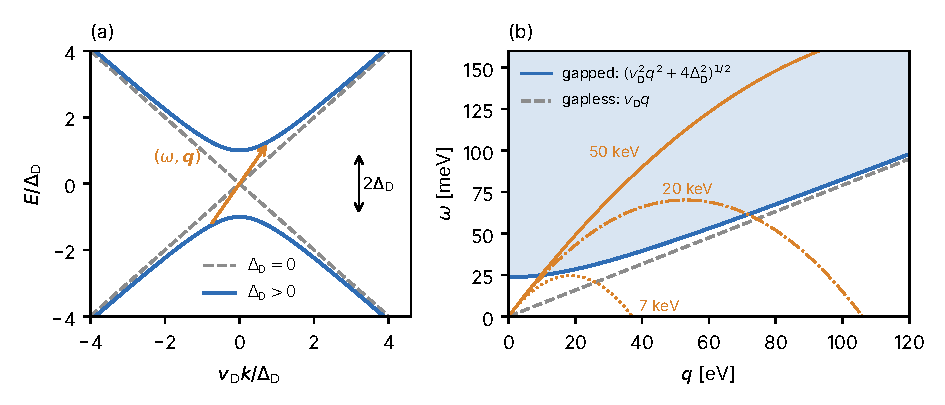
\includegraphics[width=\linewidth]{figures/ch07/fig7_3.pdf}
  \caption{Dirac cones and their pairs. (a) Bands $\pm(v_{\mathrm{D}}^2k^2 + \Delta_{\mathrm{D}}^2)^{1/2}$ of a gapped cone (solid) and of a gapless one (dashed), in units of the half-gap $\Delta_{\mathrm{D}}$; the arrow is an interband pair with energy $\omega$ and momentum $\vect{q}$. (b) Energy $\omega$ against momentum $q$ of the pairs of an isotropic cone with the ZrTe$_5$-like parameters $v_{\mathrm{D}} = 7.9\times10^{-4}$ (geometric mean of the three principal velocities) and $\Delta_{\mathrm{D}} = \SI{11.8}{meV}$ of Ref.~\cite[Table~1 and text below it]{geilhufe2020dirac}. Shaded: the pair continuum $\omega \ge (v_{\mathrm{D}}^2q^2 + 4\Delta_{\mathrm{D}}^2)^{1/2}$; dashed: its edge $\omega = v_{\mathrm{D}}q$ for $\Delta_{\mathrm{D}} = 0$. Orange: the largest energy that dark matter of mass 7, 20 and \SI{50}{keV} can deposit at momentum $q$, $\omega = qv_{\mathrm{max}} - q^2/2m_\chi$ with $v_{\mathrm{max}} = 2.650\times10^{-3}$. The \SI{7}{keV} curve stays just below the continuum; the threshold mass is \SI{8.0}{keV}.}
  \label{fig:7-dirac}
\end{figure}

Dark matter of mass $m_\chi$ can deposit at most $\omega = qv_{\mathrm{max}} - q^2/2m_\chi$ at momentum $q$ (\cref{eq:1.3-region}), and a pair is kinematically allowed where this curve enters the continuum. \Cref{fig:7-dirac}b shows that the velocity decides whether a cone can be reached at all, and the gap decides at which mass. The dark-matter curve lies below the line $\omega = v_{\mathrm{max}}q$, and the continuum edge lies above the line $\omega = v_{\mathrm{D}}q$, so that a cone with $v_{\mathrm{D}} > v_{\mathrm{max}}$ is out of reach of scattering at any mass, with or without a gap. This rules out the III--V narrow-gap semiconductors, with $v_{\mathrm{D}} \approx 1.8\,v_{\mathrm{max}}$, as scattering targets (absorption at $q \approx 0$ is another matter), and it is why the slow cones of ZrTe$_5$, at $v_{\mathrm{D}} = 0.30\,v_{\mathrm{max}}$, are of interest. In the limit $v_{\mathrm{D}} \ll v_{\mathrm{max}}$ the edge is flat at $2\Delta_{\mathrm{D}}$, and the threshold mass is that of \cref{eq:1.3-mmin} with $E_{\mathrm{th}} = 2\Delta_{\mathrm{D}}$, $m_{\mathrm{min}} = 4\Delta_{\mathrm{D}}/v_{\mathrm{max}}^2 = \SI{6.7}{keV}$ for $\Delta_{\mathrm{D}} = \SI{11.8}{meV}$. The finite velocity raises it: the smallest $m_\chi$ for which $qv_{\mathrm{max}} - q^2/2m_\chi \ge (v_{\mathrm{D}}^2q^2 + 4\Delta_{\mathrm{D}}^2)^{1/2}$ at some $q$, found numerically, is \SI{8.0}{keV} at $v_{\mathrm{D}} = 7.9\times10^{-4}$. In an anisotropic cone, $v_{\mathrm{D}}$ in \cref{eq:7.3-edge} is replaced by $(\sum_iv_i^2\hat q_i^2)^{1/2}$ for $\vect{q}$ along the unit vector $\hat{\vect{q}}$; for ZrTe$_5$ the threshold is \SI{7.1}{keV} along its slowest axis and \SI{9.6}{keV} along its fastest. The dark-matter wind arrives from a fixed direction in the Galaxy, which turns once a day in the laboratory with the rotation of the Earth, so this direction dependence is a source of daily modulation~\cite{geilhufe2020dirac}.

\subsection{Screening by Dirac electrons}

The remote bands that we dropped from \cref{eq:7.3-block} do not disappear from the response. They are the core and the bonding states of the crystal, separated from the Dirac bands by an eV or more, and at the energies $\omega \lesssim \SI{0.1}{eV}$ and momenta $q \lesssim \Lambda_{\mathrm{D}}$ that matter here they respond instantly and uniformly, like a dielectric medium. We describe them by a constant, the \emph{background dielectric constant} $\varepsilon_{\mathrm{bg}}$: the electronic dielectric constant $\varepsilon_\infty$ of \cref{sec:4.4} that the crystal would have without its Dirac electrons. In ZrTe$_5$ the remote interband transitions and the polar lattice make it large, between about 20 and 300 depending on the direction. Two charges among the Dirac electrons then interact through $e^2/(\varepsilon_{\mathrm{bg}}q^2)$, not $e^2/q^2$, and the Dirac electrons screen on top of the background. In the random-phase approximation of \cref{sec:4.5}, with $R^0_{\mathrm{D}}$ the independent-pair response of the Dirac electrons,
\begin{equation}
  \varepsilon(\vect{q},\omega) = \varepsilon_{\mathrm{bg}} - v_{\mathrm{C}}(q)\,R^0_{\mathrm{D}}(\vect{q},\omega) = \varepsilon_{\mathrm{bg}}\Bigl[1 - \frac{e^2}{\varepsilon_{\mathrm{bg}}q^2}R^0_{\mathrm{D}}(\vect{q},\omega)\Bigr] .
  \label{eq:7.3-epsbg}
\end{equation}
The bare Coulomb interaction $v_{\mathrm{C}} = e^2/q^2$ multiplies the Dirac response, and the background enters as an additive constant. Inside the bracket the Dirac electrons see the coupling $e^2/\varepsilon_{\mathrm{bg}}$. This placement of $\varepsilon_{\mathrm{bg}}$ fixes the overall size of every rate in a Dirac target, and \cref{sec:16.1} returns to it.

How strong is that coupling? A pair of Dirac electrons at distance $r$ has Coulomb energy $\alpha/(\varepsilon_{\mathrm{bg}}r)$ and kinetic energy of order $v_{\mathrm{D}}/r$, since a particle localized within $r$ has momentum $\sim 1/r$ and energy $v_{\mathrm{D}}/r$. Their ratio,
\begin{equation}
  \tilde\alpha = \frac{\alpha}{\varepsilon_{\mathrm{bg}}v_{\mathrm{D}}} ,
  \label{eq:7.3-alpha}
\end{equation}
is the same at every distance. The \emph{effective coupling} $\tilde\alpha$ plays the role that the fine-structure constant plays in quantum electrodynamics, where $v_{\mathrm{D}} = 1$ and $\varepsilon_{\mathrm{bg}} = 1$. A small velocity makes it large, and a large background constant makes it small again. For ZrTe$_5$ the two compete: $1/v_{\mathrm{D}} \approx 1300$ and $\varepsilon_{\mathrm{bg}} \approx 50$ on average, and $\tilde\alpha = 0.18$ to 0.20 with $g_{\mathrm{deg}} = 2$ (\cref{we:7-zrte5}). Part of the literature folds the degeneracy into the coupling and writes $g_{\mathrm{deg}}\alpha/(\varepsilon_{\mathrm{bg}}v_{\mathrm{D}})$ for what we write $g_{\mathrm{deg}}\tilde\alpha$~\cite[Eq.~(2.5)]{hochberg2018detection}.

\Cref{app:D.22} evaluates $R^0_{\mathrm{D}}$ for one isotropic cone at $T = 0$ with the chemical potential in the gap. Only interband pairs contribute, and each enters with the overlap of the band spinors, \cref{eq:D.22-F}, which vanishes at $q = 0$, because the two bands are orthogonal, and grows as $q^2$. That factor $q^2$ cancels the $1/q^2$ of the Coulomb interaction. In a metal the Thomas--Fermi term $k_{\mathrm{TF}}^2/q^2$ diverges as $q \to 0$; in a Dirac material the Dirac contribution to $\varepsilon$ stays finite, as it does in an insulator. The sum over $\vect{k}$ diverges logarithmically at large $\vect{k}$, for the same reason as the vacuum polarization of quantum electrodynamics, and the cutoff $|\vect{k}| < \Lambda_{\mathrm{D}}$ makes it finite. The result, \cref{eq:D.22-eps}, is
\begin{equation}
  \begin{split}
  \frac{\varepsilon(\vect{q},\omega)}{\varepsilon_{\mathrm{bg}}} = 1 + \frac{g_{\mathrm{deg}}\tilde\alpha}{6\pi}\biggl[&\ln\frac{4v_{\mathrm{D}}^2\Lambda_{\mathrm{D}}^2}{\Delta_{\mathrm{D}}^2} - \frac53 \\
  &- 6\int_0^1\dd x\,x(1 - x)\ln\Bigl(1 - x(1 - x)\frac{\omega^2 - v_{\mathrm{D}}^2q^2}{\Delta_{\mathrm{D}}^2} - \ii0^+\operatorname{sgn}\omega\Bigr)\biggr] ,
  \end{split}
  \label{eq:7.3-eps}
\end{equation}
valid for $q$, $\omega/v_{\mathrm{D}}$ and $\Delta_{\mathrm{D}}/v_{\mathrm{D}}$ small compared with $\Lambda_{\mathrm{D}}$. The response depends on $\vect{q}$ and $\omega$ only through $\omega^2 - v_{\mathrm{D}}^2q^2$, the invariant of a Lorentz transformation with $v_{\mathrm{D}}$ in place of the speed of light. It is the one-loop vacuum polarization of quantum electrodynamics with an electron of mass $\Delta_{\mathrm{D}}$, which is how Ref.~\cite[Eq.~(2.6)]{hochberg2018detection} obtained it. That reference fixes the constant inside the bracket by a subtraction at the cutoff instead of a hard cutoff, and its cutoff corresponds to $\ee^{-5/6}\Lambda_{\mathrm{D}} = 0.43\,\Lambda_{\mathrm{D}}$ in ours.

The imaginary part, which counts the pairs, needs no cutoff. For $\omega > 0$ the logarithm in \cref{eq:7.3-eps} has a negative argument inside the continuum \cref{eq:7.3-edge}, and with $s = \omega^2 - v_{\mathrm{D}}^2q^2$,
\begin{equation}
  \frac{\varepsilon_2(\vect{q},\omega)}{\varepsilon_{\mathrm{bg}}} = \frac{g_{\mathrm{deg}}\tilde\alpha}{6}\Bigl(1 - \frac{4\Delta_{\mathrm{D}}^2}{s}\Bigr)^{1/2}\Bigl(1 + \frac{2\Delta_{\mathrm{D}}^2}{s}\Bigr)\Theta(s - 4\Delta_{\mathrm{D}}^2) ,
  \label{eq:7.3-Im}
\end{equation}
which is \cref{eq:D.22-Im}. It rises from zero at the edge as the square root of the distance to it, like the density of states of a band edge, and for $s \gg \Delta_{\mathrm{D}}^2$ it tends to the constant $\varepsilon_{\mathrm{bg}}g_{\mathrm{deg}}\tilde\alpha/6$, the same at every $q$ and $\omega$. A Dirac material absorbs and scatters with a strength that, deep in the continuum, does not depend on how much energy or momentum is deposited. The flat $\varepsilon_2$ of a gapless cone, $\varepsilon_{\mathrm{bg}}g_{\mathrm{deg}}\tilde\alpha/6$ above $\omega = v_{\mathrm{D}}q$, is a signature of linear bands; optical measurements on the Dirac semimetal Na$_3$Bi agree with it to about \SI{10}{\percent}~\cite{hochberg2018detection}.

The real part carries the screening. At $q \to 0$ and $\omega = 0$ the integral in \cref{eq:7.3-eps} vanishes. The static dielectric constant of a gapped Dirac material is then \cref{eq:D.22-static},
\begin{equation}
  \varepsilon(0,0) = \varepsilon_{\mathrm{bg}}\Bigl[1 + \frac{g_{\mathrm{deg}}\tilde\alpha}{3\pi}\Bigl(\ln\frac{2v_{\mathrm{D}}\Lambda_{\mathrm{D}}}{\Delta_{\mathrm{D}}} - \frac56\Bigr)\Bigr] .
  \label{eq:7.3-static}
\end{equation}
The Dirac electrons add to the background a term proportional to $g_{\mathrm{deg}}\tilde\alpha$ times a logarithm of the ratio of the band width $v_{\mathrm{D}}\Lambda_{\mathrm{D}}$ to the gap. Pairs of every energy between $2\Delta_{\mathrm{D}}$ and $2v_{\mathrm{D}}\Lambda_{\mathrm{D}}$ contribute equally per logarithmic interval, which is where the logarithm comes from. The dependence on the cutoff is mild: doubling $\Lambda_{\mathrm{D}}$ changes $\varepsilon(0,0)/\varepsilon_{\mathrm{bg}}$ by $g_{\mathrm{deg}}\tilde\alpha\ln2/3\pi$, under \SI{3}{\percent} for ZrTe$_5$. And the split between $\varepsilon_{\mathrm{bg}}$ and the Dirac term is not unique. States beyond $\Lambda_{\mathrm{D}}$ belong to the background, so a larger cutoff moves weight from $\varepsilon_{\mathrm{bg}}$ into the logarithm, and only the total $\varepsilon$ is measurable.

As $q$ grows at $\omega = 0$, the argument of the logarithm in \cref{eq:7.3-eps} grows and the screening weakens. Once $v_{\mathrm{D}}q \gg 2\Delta_{\mathrm{D}}$ the gap no longer matters, and the result approaches that of a gapless cone.
\begin{limitbox}[Dielectric function of a gapless Dirac material][lim:7.3a]
For $\Delta_{\mathrm{D}} \to 0$, with a hard momentum cutoff $\Lambda_{\mathrm{D}}$, $\varepsilon/\varepsilon_{\mathrm{bg}} = 1 + (g_{\mathrm{deg}}\tilde\alpha/6\pi)\ln[4\Lambda_{\mathrm{D}}^2/|q^2 - \omega^2/v_{\mathrm{D}}^2|] + \ii(g_{\mathrm{deg}}\tilde\alpha/6)\,\Theta(\omega - v_{\mathrm{D}}q)$, after~\cite[Eq.~(2.7)]{hochberg2018detection}.
\par\smallskip
{\centering
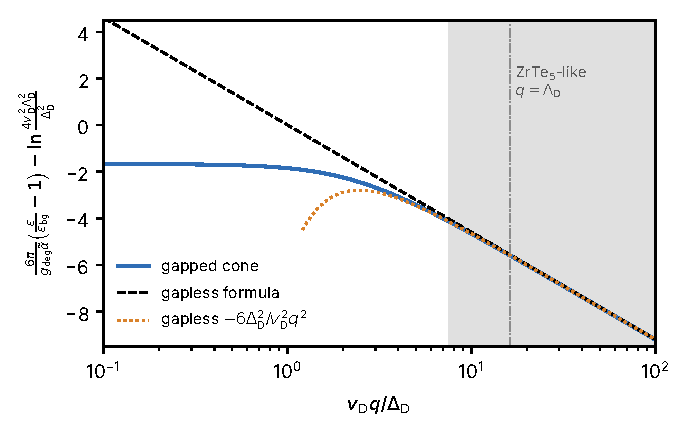
\includegraphics[width=\linewidth]{figures/ch07/limit7_gapless.pdf}
\captionof{figure}{Static dielectric function of a gapped Dirac cone against the gapless formula. Plotted is the induced part $\varepsilon(q,0)/\varepsilon_{\mathrm{bg}} - 1$ in units of $g_{\mathrm{deg}}\tilde\alpha/6\pi$, less the cutoff term $\ln(4v_{\mathrm{D}}^2\Lambda_{\mathrm{D}}^2/\Delta_{\mathrm{D}}^2)$, which makes the curves independent of the cutoff (hard cutoff on $|\vect{k}|$). Solid: \cref{eq:7.3-eps} at $\omega = 0$; dashed: the gapless formula, $-2\ln(v_{\mathrm{D}}q/\Delta_{\mathrm{D}})$ on this scale; dotted: the gapless formula with its leading correction $-6\Delta_{\mathrm{D}}^2/v_{\mathrm{D}}^2q^2$. Gray: $v_{\mathrm{D}}q > 7.5\,\Delta_{\mathrm{D}}$, where the gapless formula is within 0.1 of the full result; with the correction this holds from $3.7\,\Delta_{\mathrm{D}}$, and at $v_{\mathrm{D}}q = 10\,\Delta_{\mathrm{D}}$ the residual is $3\times10^{-3}$. Dash-dotted: $q = \Lambda_{\mathrm{D}}$ for the ZrTe$_5$-like cone of \cref{we:7-zrte5}, where $v_{\mathrm{D}}\Lambda_{\mathrm{D}} = 16.2\,\Delta_{\mathrm{D}}$. The Dirac region ends there.}\label{fig:7-gapless-limit}
\par}
\smallskip
Below $v_{\mathrm{D}}q \approx 2\Delta_{\mathrm{D}}$ the gapless formula diverges logarithmically, while the gapped cone saturates at \cref{eq:7.3-static}: the gap cuts off the pairs that would screen at long wavelength.
\end{limitbox}
The gapless formula follows from \cref{eq:7.3-eps} by expanding the logarithm for $|s| \gg \Delta_{\mathrm{D}}^2$: $\ln[1 - x(1 - x)s/\Delta_{\mathrm{D}}^2] \to \ln[-x(1 - x)s/\Delta_{\mathrm{D}}^2] + \Delta_{\mathrm{D}}^2/[-x(1 - x)s]$, and with $\int_0^1x(1 - x)\ln[x(1 - x)]\,\dd x = -5/18$ the constants $-\frac53$ cancel and $\Delta_{\mathrm{D}}$ drops out of the logarithm (\cref{eq:D.22-gapless}). The next term contributes $-6\Delta_{\mathrm{D}}^2/(v_{\mathrm{D}}^2q^2 - \omega^2)$ to the bracket. Static screening in a gapless cone, $\varepsilon(q,0) = \varepsilon_{\mathrm{bg}}[1 + (g_{\mathrm{deg}}\tilde\alpha/3\pi)\ln(2\Lambda_{\mathrm{D}}/q)]$, grows without bound as $q \to 0$, but only logarithmically. There is no screening length, since the density of states vanishes at the node; the electron gas screens a charge completely beyond $1/k_{\mathrm{TF}}$, whereas a gapless Dirac material only reduces it by a slowly growing factor.

The logarithms also set the validity of the calculation. The random-phase approximation keeps the first term in $\tilde\alpha$ of the polarization, and the induced part of \cref{eq:7.3-eps} is of order $g_{\mathrm{deg}}\tilde\alpha\ln(v_{\mathrm{D}}\Lambda_{\mathrm{D}}/\max(\Delta_{\mathrm{D}}, v_{\mathrm{D}}q))$, up to the numerical factor $1/3\pi$. We take this product as the expansion parameter: perturbation theory is reliable when it is small compared with one. Reading the screened interaction $e^2/\varepsilon q^2$ as a coupling that depends on $q$, the screening makes it weaker at smaller $q$, the counterpart of the running of the fine-structure constant in quantum electrodynamics, and the theory becomes weakly coupled at long wavelength~\cite{hochberg2018detection}. For $\tilde\alpha \gtrsim 1$ the one-loop result is an estimate, and what replaces it is an open question that \cref{sec:16.1} takes up.

Anisotropy enters through a rescaling. With $\delta k_i \to \delta k_i/v_i$, the Hamiltonian \cref{eq:7.3-H} becomes isotropic with unit velocity, the sum over $\vect{k}$ acquires the Jacobian $1/(v_1v_2v_3)$, and $q^2$ in the overlap becomes $\sum_iv_i^2q_i^2$ (\cref{app:D.22}). The cutoff becomes an ellipsoid in $\vect{k}$, a sphere of radius $\Lambda_{\mathrm{D}}v_{\mathrm{D}}$ in energy units for the rescaled momenta. For $\vect{q}$ along the principal axis $i$, the Coulomb factor $e^2/q^2$ then multiplies $v_i^2/(v_1v_2v_3)$ in place of $1/v_{\mathrm{D}}$, and the background constant becomes its component $\varepsilon_{\mathrm{bg},ii}$ along that axis, assuming the background and the cone share principal axes. The static constant along $i$ is
\begin{equation}
  \varepsilon_{ii}(0,0) = \varepsilon_{\mathrm{bg},ii} + \frac{g_{\mathrm{deg}}\alpha}{3\pi}\,\frac{v_i^2}{v_1v_2v_3}\Bigl(\ln\frac{2\tilde\Lambda}{\Delta_{\mathrm{D}}} - \frac56\Bigr) ,
  \label{eq:7.3-aniso}
\end{equation}
with $\tilde\Lambda$ the cutoff on the energy $(\sum_iv_i^2\delta k_i^2)^{1/2}$. Along each axis the effective coupling is $\alpha v_i^2/(\varepsilon_{\mathrm{bg},ii}v_1v_2v_3)$, which reduces to \cref{eq:7.3-alpha} for an isotropic cone.

The four inputs of \cref{eq:7.3-eps}, $v_i$, $\Delta_{\mathrm{D}}$, $\Lambda_{\mathrm{D}}$ and $\varepsilon_{\mathrm{bg}}$, come from first-principles calculations. The velocities and the cutoff are fitted to a computed band structure near the node (\cref{app:E.1}). The half-gap is the delicate one: semilocal functionals misplace small gaps and can invert the band order, and quasiparticle corrections (\cref{app:E.3}) or the measured gap are needed. The background constant comes from density-functional perturbation theory (\cref{app:E.4}) or from the random-phase sum over bands (\cref{app:E.6}). Both compute the dielectric constant of the whole crystal, which includes the Dirac pairs, and they do so at the calculated gap, to which the Dirac term is sensitive through $\ln(1/\Delta_{\mathrm{D}})$. A consistent $\varepsilon_{\mathrm{bg}}$ leaves the Dirac bands out of the sum over transitions, or subtracts \cref{eq:7.3-static} from the computed total. The parameters of ZrTe$_5$ used in rate calculations are specified in \cref{app:E.20}.

\begin{workedexample}{Effective coupling and static screening of ZrTe$_5$}\label{we:7-zrte5}
ZrTe$_5$ has one gapped cone at $\mathrm{\Gamma}$, $g_{\mathrm{deg}} = 2$. We take the first-principles values for the measured crystal structure~\cite[Table~1 and text below it]{geilhufe2020dirac}. They are the principal velocities $v_x, v_y, v_z = 1.1\times10^{-3}$, $4.5\times10^{-4}$, $1.0\times10^{-3}$, a gap of \SI{23.6}{meV} ($\Delta_{\mathrm{D}} = \SI{11.8}{meV}$), and cutoffs $\Lambda_x, \Lambda_y, \Lambda_z = 0.23$, $0.215$, \SI{0.1}{\angstrom^{-1}}. A relaxed cell volume gives the same $v_x$, slower $v_y = 4.4\times10^{-4}$ and $v_z = 9.1\times10^{-4}$, and a gap of \SI{31.2}{meV} ($\Delta_{\mathrm{D}} = \SI{15.6}{meV}$); the reference implements that row in its rates. The dielectric tensor from density-functional perturbation theory has the diagonal components 308.4, 20.75 and 126.1~\cite[Table~2]{geilhufe2020dirac}.

\emph{Cutoff.} With $\SI{1}{\angstrom^{-1}} = \SI{1.973}{keV}$, the band energies at the three cutoffs are $v_i\Lambda_i = 0.499$, $0.191$ and \SI{0.197}{eV}. The cone is linear to a much higher energy along $x$ than along $y$. We keep the states with $(\sum_iv_i^2\delta k_i^2)^{1/2} < \tilde\Lambda = \SI{0.191}{eV}$, the smallest of the three~\cite[Eq.~(2.21)]{geilhufe2020dirac}, a conservative choice that a better fit of the bands would replace by a larger ellipsoid. Their dielectric function, Ref.~\cite[Eq.~(3.10)]{geilhufe2020dirac}, carries the same constant $-\frac53$ as \cref{eq:7.3-eps}, so that $\tilde\Lambda$ is a hard cutoff in our sense, $\tilde\Lambda = v_{\mathrm{D}}\Lambda_{\mathrm{D}}$.

\emph{Isotropic estimate.} To get a single number, replace the cone by an isotropic one with the same density of states, $v_{\mathrm{D}} = (v_xv_yv_z)^{1/3} = 7.9\times10^{-4}$, and the tensor by the harmonic mean of its components, $\varepsilon_{\mathrm{bg}} = 3/(\sum_i1/\varepsilon_{\mathrm{bg},ii}) = 50.5$, the average used in Ref.~\cite{hochberg2018detection}. Then \cref{eq:7.3-alpha} gives $\tilde\alpha = 0.18$ and $g_{\mathrm{deg}}\tilde\alpha = 0.37$. The cutoff in momentum is $\Lambda_{\mathrm{D}} = \tilde\Lambda/v_{\mathrm{D}} = \SI{241}{eV} = \SI{0.12}{\angstrom^{-1}}$. An earlier calculation~\cite[Table~1]{hochberg2018detection}, with faster velocities ($2.9\times10^{-3}$, $5.0\times10^{-4}$, $2.1\times10^{-3}$) and smaller dielectric constants (187.5, 9.8 and 90.9, harmonic mean 25.3), yields a similar $\tilde\alpha = 0.20$, quoted there as $g_{\mathrm{deg}}\tilde\alpha = 0.80$ with $g_{\mathrm{deg}} = 4$ states per band.

\emph{Static screening.} With $\ln(2\tilde\Lambda/\Delta_{\mathrm{D}}) = \ln 32.4 = 3.48$, \cref{eq:7.3-static} yields
\begin{equation*}
  \frac{\varepsilon(0,0)}{\varepsilon_{\mathrm{bg}}} - 1 = \frac{0.37}{3\pi}\,(3.48 - 0.83) = 0.102 ,
\end{equation*}
so that $\varepsilon(0,0) = 55.7$. The Dirac electrons add \SI{10}{\percent} to the screening of the background. At finite $q$, the integral in \cref{eq:7.3-eps} reduces this to 0.091 at $q = 2\Delta_{\mathrm{D}}/v_{\mathrm{D}} = \SI{30}{eV}$ and to 0.052 at $q = \Lambda_{\mathrm{D}}/2 = \SI{121}{eV}$, momenta at which sub-MeV dark matter scatters (\cref{fig:7-dirac}b). The expansion parameter at long wavelength, $g_{\mathrm{deg}}\tilde\alpha\ln(v_{\mathrm{D}}\Lambda_{\mathrm{D}}/\Delta_{\mathrm{D}}) = 0.37\ln 16.2 = 1.0$, is about one. The induced term itself, 0.102, is small mainly through the factor $1/3\pi$, and the one-loop result is a fair estimate of it. Since $v_{\mathrm{D}}\Lambda_{\mathrm{D}} = 16.2\,\Delta_{\mathrm{D}}$, ZrTe$_5$ reaches the gapless regime of \cref{fig:7-gapless-limit} only above $v_{\mathrm{D}}q = 7.5\,\Delta_{\mathrm{D}}$, or $q = \SI{112}{eV}$: below that momentum the gap matters.

\emph{Anisotropy.} Along the principal axes, \cref{eq:7.3-aniso} with $\ln(2\tilde\Lambda/\Delta_{\mathrm{D}}) - \frac56 = 2.64$ adds 10.0, 1.67 and 8.3 to the background components 308.4, 20.75 and 126.1, that is 3.2, 8.1 and \SI{6.6}{\percent}. The effective couplings along the three axes, $\alpha v_i^2/(\varepsilon_{\mathrm{bg},ii}v_xv_yv_z)$, are 0.058, 0.144 and 0.117: the slow direction $y$ has the smallest background constant as well, and it is the most strongly coupled. The averaged $\tilde\alpha = 0.18$ is a fair summary, though it overstates the coupling along $x$ threefold.

\emph{Size of the Dirac screening.} The Dirac contribution is 3 to \SI{8}{\percent} of the dielectric constant, smaller than the spread between the two sets of computed parameters. Both sets of dielectric constants are totals for the whole crystal, computed at a gap of 24 to \SI{35}{meV}, and already contain a Dirac term of this size, which is harmless at the few-percent level. The coupling that matters for a rate is the total $\varepsilon$, dominated here by the background: with $\varepsilon \approx 56$, every Coulomb-like interaction inside ZrTe$_5$ is reduced about fifty-fold.
\end{workedexample}

Dirac materials screen the interaction mostly through their large background dielectric constant, with the Dirac electrons adding a logarithm of order $g_{\mathrm{deg}}\tilde\alpha$. The loss function that follows from \cref{eq:7.3-eps}, and the rates of scattering and absorption with the background placed in the total $\varepsilon$ as in \cref{eq:7.3-epsbg}, are the subject of \cref{sec:16.1}.

\section{Defects and dopants}\label{sec:7.4}

A phosphorus atom in silicon binds its fifth electron by \SI{45.6}{meV}, a twenty-fifth of the gap. Dark matter of \SI{13}{keV} carries enough kinetic energy to set that electron free, where the gap of the perfect crystal needs \SI{0.333}{MeV} (\cref{sec:1.3}). A carbon--hydrogen complex in the same crystal, the T center, emits light at \SI{935}{meV}, and a quarter of its photons leave without exciting a single phonon. And a silicon atom struck with a few tens of eV leaves its site for good, storing several eV in the vacancy and the interstitial it leaves behind. Defects therefore enter a dark-matter experiment in two roles: as targets with their own low thresholds, and as final states or readouts of an energy deposit. Each is built from formalism already in hand. The shallow donor is the hydrogenic envelope of \cref{sec:4.9} with the valley masses of \cref{sec:3.3}, the color center is the displaced oscillator of \cref{sec:5.6}, and the displacement threshold is a property of the energy surface of \cref{sec:5.1}.

\subsection{Shallow donors}

An atom from group V on a silicon site, such as phosphorus, arsenic or antimony, uses four of its five valence electrons in the bonds. The fifth is bound to the ion core and its one extra positive charge, in a hydrogenic donor level just below the conduction band, built from conduction-band states. An impurity of this kind is a \emph{donor}; a group-III atom such as boron, one electron short, binds a hole instead and is an \emph{acceptor}. Both bind their carrier weakly, because the host screens the Coulomb attraction by the static dielectric constant $\varepsilon_0$ and the carrier moves with the band mass $m^*$ rather than $m_e$.

The hydrogen atom with these two substitutions already sets the scale. \Cref{app:D.23} derives the envelope equation of Kohn and Luttinger~\cite{kohn1955theory} and~\cite[Chap.~4]{yu2010fundamentals}. The donor potential varies slowly on the scale of the lattice and mixes only conduction states within $\sim 1/a^*$ of a band minimum $\vect{k}_j$. The donor state is then the Bloch function at the minimum modulated by an envelope,
\begin{equation}
  \psi(\vect{r}) \simeq F_j(\vect{r})\,\psi_{c\vect{k}_j}(\vect{r}) , \qquad
  \Bigl[-\frac{\partial_x^2 + \partial_y^2}{2m^*_\perp} - \frac{\partial_z^2}{2m^*_\parallel} - \frac{\alpha}{\varepsilon_0 r}\Bigr]F_j(\vect{r}) = -E_{\mathrm{b}}^{\mathrm{D}}\,F_j(\vect{r}) ,
  \label{eq:7.4-EMT}
\end{equation}
with $z$ along the axis of the valley and $E_{\mathrm{b}}^{\mathrm{D}}$ the \emph{donor binding energy}, measured down from the conduction-band minimum. This is \emph{effective-mass theory}. It is the Wannier--Mott equation \cref{eq:4.9-envelope} with two changes. The electron is bound to a fixed ion rather than to a hole, which makes the mass the band mass and not a reduced mass. And the mass is a tensor, because the valleys of silicon are ellipsoids (\cref{sec:3.3}).

\begin{keyresult}[Effective-mass donor levels]
For an isotropic mass $m^*$ the solution of \cref{eq:7.4-EMT} is hydrogenic, with the \emph{effective Bohr radius} $a^*$,
\begin{equation}
  E_{\mathrm{b}}^{\mathrm{D}} = \frac{m^*\alpha^2}{2\varepsilon_0^2} = \frac{m^*/m_e}{\varepsilon_0^2}\,\mathrm{Ry} , \qquad
  a^* = \frac{\varepsilon_0}{m^*\alpha} = \varepsilon_0\,\frac{m_e}{m^*}\,a_0 ,
  \label{eq:7.4-hydrogenic}
\end{equation}
and excited levels at $E_{\mathrm{b}}^{\mathrm{D}}/n^2$ below the band edge.
\end{keyresult}
With $\varepsilon_0 = 11.7$ and masses of a few tenths of $m_e$, the binding is tens of meV and the orbit tens of \si{\angstrom}, several lattice constants. The assumption behind \cref{eq:7.4-EMT}, an envelope spread over many cells, is then satisfied, which makes the estimate self-consistent. For silicon the estimate brackets the answer without giving it: the transverse mass $m^*_\perp = 0.191\,m_e$ puts the binding at \SI{19.0}{meV} and $a^* = \SI{32.4}{\angstrom}$, the longitudinal mass $m^*_\parallel = 0.916\,m_e$ at \SI{91.0}{meV} and \SI{6.8}{\angstrom}.

The anisotropic problem has one parameter, the mass ratio $\gamma_m = m^*_\perp/m^*_\parallel = 0.209$. In units of the transverse Rydberg $\mathrm{Ry}^*_\perp = m^*_\perp\alpha^2/2\varepsilon_0^2 = \SI{18.98}{meV}$ and radius $a^*_\perp = \SI{32.4}{\angstrom}$, the variational envelope of Kohn and Luttinger, a hydrogen $1s$ function squeezed along the heavy axis, binds the electron by $E_{\mathrm{b}}^{\mathrm{D}} = 1.564\,\mathrm{Ry}^*_\perp = \SI{29.7}{meV}$, with the radii $r_\perp = \SI{24.3}{\angstrom}$ across the valley axis and $r_\parallel = \SI{14.0}{\angstrom}$ along it (\cref{eq:D.23-Si}). The orbit is an oblate spheroid, flattened along the heavy direction, where the electron is less mobile, and the binding lies between the two isotropic values, closer to the light one, because two of the three directions are light. The full spectrum of \cref{eq:7.4-EMT} needs a numerical solution. Scaling $z$ by $\gamma_m^{1/2}$ makes the kinetic energy isotropic and turns the Coulomb potential into $-2/[r\,(1 - (1 - \gamma_m)\cos^2\theta)^{1/2}]$ in these units. Expanding that angular factor in Legendre polynomials, and the envelope in spherical harmonics of fixed $m$ and parity, leaves a set of coupled radial equations, which we solve on a grid. The ground state comes out at $1.566\,\mathrm{Ry}^*_\perp = \SI{29.7}{meV}$, so the variational envelope is within \num{0.002} $\mathrm{Ry}^*_\perp$ of the exact effective-mass ground state. The excited states are labeled by their hydrogenic parents; the anisotropy splits each $np$ level into $np_0$, with the node across the valley axis, and $np_\pm$. \Cref{fig:7-donor} shows them.

\begin{figure}[t]
  \centering
  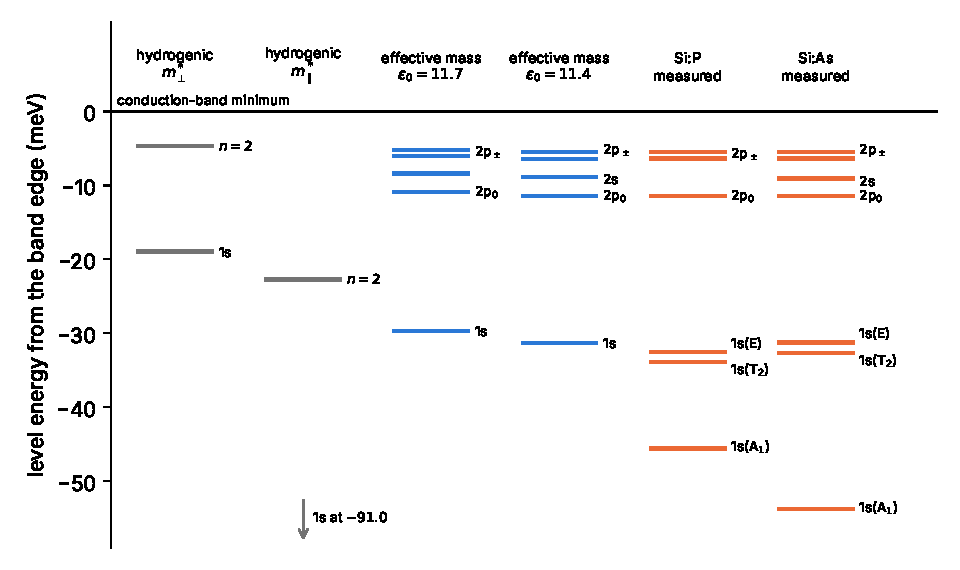
\includegraphics[width=\linewidth]{figures/ch07/fig7_4.pdf}
  \caption{Bound levels of a shallow donor in silicon, measured from the conduction-band minimum (meV). Gray: the hydrogenic model, \cref{eq:7.4-hydrogenic}, with $\varepsilon_0 = 11.7$ and the transverse mass $0.191\,m_e$ ($1s$ at \SI{19.0}{meV}) or the longitudinal mass $0.916\,m_e$ ($1s$ at \SI{91.0}{meV}, off the scale), each with its $n = 2$ level. Blue: the effective-mass equation \cref{eq:7.4-EMT} with both masses, solved numerically (coupled radial equations in spherical harmonics after scaling $z$ by $\gamma_m^{1/2}$, $l \le 14$), for $\varepsilon_0 = 11.7$ (room temperature) and 11.4 (liquid-helium temperature); from the top, $3p_0$, $2p_\pm$, $2s$, $2p_0$ and $1s$. Orange: measured levels of phosphorus and arsenic donors~\cite[Fig.~1]{vinh2008silicon}. The $p$ levels agree with effective-mass theory at $\varepsilon_0 = 11.4$ to \SI{0.4}{\percent}; the $1s$ level splits into $A_1$, $T_2$ and $E$ states, and the $A_1$ ground state lies below the effective-mass value by \SI{14}{meV} for phosphorus and \SI{22}{meV} for arsenic.}
  \label{fig:7-donor}
\end{figure}

The measured spectra test the theory state by state~\cite[Fig.~1]{vinh2008silicon}. The $p$ levels of phosphorus and arsenic agree with each other to \SI{0.02}{meV}: $2p_0$ at 11.48 and \SI{11.50}{meV}, $2p_\pm$ at \SI{6.40}{meV} for both. They do not depend on the chemistry of the donor, as effective-mass theory says they should. With $\varepsilon_0 = 11.7$, however, the theory puts them \SI{5}{\percent} too shallow, at 10.92 and \SI{6.09}{meV}. Since every level of \cref{eq:7.4-EMT} scales as $1/\varepsilon_0^2$, the measured $2p_\pm$ fixes $\varepsilon_0 = 11.7\times(6.09/6.40)^{1/2} = 11.4$. It is the value of the static constant at liquid-helium temperature, where donor spectra are taken, that calculations of donor levels use~\cite{faulkner1969higher,smith2017ab}, \SI{2.6}{\percent} below the room-temperature 11.7. With 11.4, effective-mass theory puts $2p_0$, $2p_\pm$ and $3p_0$ at 11.51, 6.42 and \SI{5.49}{meV}, within \SI{0.4}{\percent} of the measured 11.48, 6.40 and \SI{5.47}{meV}, and the $1s$ state at \SI{31.3}{meV}, the value Faulkner obtained~\cite{faulkner1969higher,smith2017ab}. The $p$ envelopes vanish at the donor site and never see the ion core.

The ground states are another matter. Phosphorus binds its electron by \SI{45.59}{meV}~\cite{jagannath1981linewidths}, arsenic by \SI{53.76}{meV}~\cite[Fig.~1]{vinh2008silicon}, and antimony by \SI{42.7}{meV}~\cite[Table~3]{claes2025accurate}, all deeper than \SI{31.3}{meV} and different from one another. The difference lies near the core. Within a lattice constant of the donor the screening by $\varepsilon_0$ is incomplete, and the potential carries the chemistry of the ion; the envelope equation replaces both by $-\alpha/\varepsilon_0 r$. The $1s$ envelope is largest exactly there, and the potential that \cref{eq:7.4-EMT} leaves out shifts it. This shift is the \emph{central-cell correction}.

The central cell also lifts a degeneracy that the effective-mass equation leaves intact. Silicon has six valleys, on the $\langle100\rangle$ axes, and each carries its own envelope, rotated with its axis; at the order of \cref{eq:7.4-EMT}, any combination $\sum_jc_jF_j\psi_{c\vect{k}_j}$ is a ground state, sixfold degenerate without spin. The short-range part of the donor potential couples the valleys, because a potential concentrated in one cell has Fourier components at the large momenta $\vect{k}_j - \vect{k}_{j'}$ between them. The donor site has the symmetry of a regular tetrahedron, the point group $T_d$, which leaves three matrix elements, $\Delta_0$ within a valley, $\Delta_{\mathrm{g}}$ between opposite valleys and $\Delta_{\mathrm{f}}$ between perpendicular ones. The six states split into a singlet $A_1$, a doublet $E$ and a triplet $T_2$. These are the standard names of the irreducible representations of $T_d$: each label says how a set of states transforms under the rotations and reflections of the tetrahedron, and here it fixes the degeneracy, one, two or three. The levels lie at
\begin{equation}
  E_{A_1} = \Delta_0 + \Delta_{\mathrm{g}} + 4\Delta_{\mathrm{f}} , \qquad
  E_E = \Delta_0 + \Delta_{\mathrm{g}} - 2\Delta_{\mathrm{f}} , \qquad
  E_{T_2} = \Delta_0 - \Delta_{\mathrm{g}} ,
  \label{eq:7.4-vo}
\end{equation}
relative to the effective-mass level (\cref{eq:D.23-vo}). In the $A_1$ state all six valleys add in phase at the donor site; it has the largest density on the core and an attractive central cell lowers it most. This \emph{valley-orbit splitting} is what the measured spectra show: the phosphorus $1s$ level is a singlet at \SI{45.59}{meV}, with the triplet $T_2$ at \SI{33.89}{meV} and the doublet $E$ at \SI{32.58}{meV}, close to the effective-mass value~\cite[Fig.~1]{vinh2008silicon}. The central-cell correction is a property of the $s$-like ground state, and a large one, a third of the binding of phosphorus.

The donor's size sets the density at which it stays a single donor. The \emph{defect density} $\nd_{\mathrm{D}}$, the number of donors (or of any defect) per unit volume, has to be small enough that orbits do not overlap, $\nd_{\mathrm{D}}a^{*3} \ll 1$. The spheroid of radii $r_\perp$, $r_\perp$ and $r_\parallel$ has a volume of \SI{3.5e-20}{cm^3}, and one donor per orbit means $\nd_{\mathrm{D}} \approx \SI{3e19}{cm^{-3}}$. In a lightly doped crystal, with $\nd_{\mathrm{D}} = \SI{e15}{cm^{-3}}$, donors sit \SI{100}{nm} apart and each is an isolated hydrogen atom of the crystal. At higher densities the electrons hop between donors and form an impurity band, and the isolated-donor picture fails before the orbits touch, at the Mott metal--insulator transition.

Acceptors are bound by similar amounts, tens of meV in silicon, but their effective-mass problem is harder. The valence maximum is degenerate, with heavy and light holes and a split-off band (\cref{sec:3.3}), and \cref{eq:7.4-EMT} becomes a set of coupled equations for several envelopes, the same complication that the heavy--light mixing brings to excitons (\cref{sec:4.9}). Donors are the cleaner case, and we keep to them.

Effective-mass theory is the computational method of choice for shallow donors, because no supercell is large enough to hold the envelope. An orbit of radius \SI{2.4}{nm} spans thousands of atoms, and a supercell calculation of the donor (\cref{app:E.10}) has to extrapolate in its size. It also inherits the error of its functional, magnified: a semilocal functional spreads the donor electron too far and binds phosphorus by only \SI{19.2}{meV} after extrapolation, against the measured \SI{45.6}{meV}~\cite[Table~3]{claes2025accurate}. What a supercell supplies well is the potential within a cell or two of the core. Combined with the envelope equation, in multivalley effective-mass theory, that potential gives the central-cell correction and the valley-orbit splitting, which is the division of labor that \cref{app:D.23} sets up.

\begin{workedexample}{The binding of phosphorus in silicon}\label{we:7-sip}
We compare the effective-mass binding of a phosphorus donor with the measured \SI{45.59}{meV} and extract the valley-orbit matrix elements, with the masses $m^*_\perp = 0.191\,m_e$ and $m^*_\parallel = 0.916\,m_e$ of \cref{tab:3-materials}.

\emph{Units.} With $\varepsilon_0 = 11.7$, $\mathrm{Ry}^*_\perp = 0.191\times\SI{13606}{meV}/11.7^2 = \SI{18.98}{meV}$, $a^*_\perp = 11.7\times\SI{0.529}{\angstrom}/0.191 = \SI{32.4}{\angstrom}$ and $\gamma_m = 0.209$.

\emph{Effective-mass ground state.} The variational envelope of \cref{app:D.23} binds the electron by \SI{29.7}{meV}, and the numerical solution of \cref{eq:7.4-EMT} gives $1.566\,\mathrm{Ry}^*_\perp$, also \SI{29.7}{meV}. At the liquid-helium value $\varepsilon_0 = 11.4$, which the $p$ levels require, $\mathrm{Ry}^*_\perp = \SI{20.00}{meV}$ and the effective-mass $1s$ level lies at \SI{31.3}{meV}.

\emph{Central-cell correction.} The measured ground state is $\SI{45.59}{meV} - \SI{31.3}{meV} = \SI{14.3}{meV}$ deeper, \SI{31}{\percent} of the binding. The measured binding itself leans on the theory: the spectroscopy measures transitions, and the absolute ground-state energy follows by adding the effective-mass binding of a high $p$ state, \SI{3.12}{meV} for $3p_\pm$, to the measured $1s(A_1) \to 3p_\pm$ line~\cite{smith2017ab}. The $p$ levels can bear that weight, as \cref{fig:7-donor} shows.

\emph{Valley-orbit matrix elements.} Taking the effective-mass level $-\SI{31.3}{meV}$ as the reference, the three measured $1s$ levels of phosphorus, $A_1$ at $-45.59$, $T_2$ at $-33.89$ and $E$ at \SI{-32.58}{meV}, sit at $-14.29$, $-2.59$ and \SI{-1.28}{meV}. \Cref{eq:7.4-vo} gives $E_{A_1} - E_E = 6\Delta_{\mathrm{f}}$, so $\Delta_{\mathrm{f}} = -13.01/6 = \SI{-2.17}{meV}$; then $\Delta_0 + \Delta_{\mathrm{g}} = E_E + 2\Delta_{\mathrm{f}} = \SI{-5.62}{meV}$ and $\Delta_0 - \Delta_{\mathrm{g}} = E_{T_2} = \SI{-2.59}{meV}$, so that $\Delta_0 = \SI{-4.10}{meV}$ and $\Delta_{\mathrm{g}} = \SI{-1.51}{meV}$. All three are negative, as an attractive core requires, and the coupling between perpendicular valleys is the larger of the two intervalley terms. The $E$ and $T_2$ states lie only 1.3 and \SI{2.6}{meV} below the effective-mass value, and the $A_1$ state takes \SI{14.3}{meV}, because only $A_1$ collects all six valleys in phase at the core.

\emph{Size.} The variational envelope of \cref{app:D.23} has $|F(0)|^2 = 1/(\pi r_\perp^2r_\parallel)$, with the radii $r_\perp = \SI{24.3}{\angstrom}$ and $r_\parallel = \SI{14.0}{\angstrom}$ found above. The volume of one silicon atom is $a^3/8$, with the lattice constant $a = \SI{5.43}{\angstrom}$, and the probability of finding the electron within it around the donor is $|F(0)|^2a^3/8 = (\SI{5.43}{\angstrom})^3/(8\pi\times24.3^2\times\SI{14.0}{\angstrom^3}) = \num{7.7e-4}$ per valley envelope. The central cell is a small region of the orbit, and still it moves the ground state by a third: the potential there is that of an unscreened ion, many eV deep.

\emph{Kinematics.} Dark matter can ionize the donor if $\tfrac12\mchi v_{\mathrm{max}}^2 \ge E_{\mathrm{b}}^{\mathrm{D}}$, that is for $\mchi \ge 2\times\SI{45.59}{meV}/\num{7.023e-6} = \SI{13.0}{keV}$, twenty-six times lighter than the \SI{0.333}{MeV} of the silicon gap. At threshold the momentum transfer is $\mchi v_{\mathrm{max}} = \SI{34.4}{eV}$. The envelope spreads over momenta up to $1/r_\perp = \SI{81}{eV}$ across the valley axis and $1/r_\parallel = \SI{141}{eV}$ along it, so $qr_\perp \approx 0.42$: the dark matter that can just ionize the donor transfers momenta that the bound electron has. In the language of \cref{sec:1.3}, the donor is a good kinematic match to dark matter of a few tens of keV.
\end{workedexample}

\subsection{Color centers}

The T center of silicon emits at \SI{935}{meV}, \SI{1326}{nm} in the telecommunications O band, and the nitrogen--vacancy center of diamond at \SI{1.945}{eV}, \SI{637}{nm}. Both lines are sharp, and both sit on a broad band of lower-energy light. Defects of this kind are called \emph{color centers}, after the F centers that color the alkali halides. Their levels lie deep in the gap, and their electrons are confined within a cell or two of the defect, unlike the donor electron of the previous subsection. A localized electron that changes its state exerts large forces on the few atoms around it. The nuclei settle at different positions in the ground and the excited state, and an optical transition, which is fast compared with the nuclear motion, leaves them displaced from their new equilibrium. This is the displaced oscillator of \cref{sec:5.6}, and color centers are where its parameters are measured.

The \emph{configuration-coordinate diagram} draws the two Born--Oppenheimer surfaces of \cref{sec:5.1}, one for each electronic state, along the single coordinate $Q$ that connects their minima. With $Q$ mass-weighted, as $\Delta Q = M^{1/2}\Delta x$ in \cref{sec:5.6}, and one effective mode of energy $\omega_0$ that is the same in both states,
\begin{equation}
  E^{\mathrm{ad}}_{\mathrm{g}}(Q) = \tfrac12\omega_0^2Q^2 , \qquad
  E^{\mathrm{ad}}_{\mathrm{e}}(Q) = E_{\mathrm{ZPL}} + \tfrac12\omega_0^2(Q - \Delta Q)^2 , \qquad
  S_{\mathrm{HR}} = \tfrac12\omega_0\Delta Q^2 .
  \label{eq:7.4-cc}
\end{equation}
The \emph{zero-phonon-line energy} $E_{\mathrm{ZPL}}$ is the difference between the two minima, the energy of the transition that leaves the vibrational state unchanged, and the Huang--Rhys factor $S_{\mathrm{HR}}$ measures the displacement in units of the zero-point spread of the mode. A vertical transition from the ground minimum lands $\tfrac12\omega_0^2\Delta Q^2 = S_{\mathrm{HR}}\omega_0$ above the excited minimum, so absorption peaks near $E_{\mathrm{ZPL}} + S_{\mathrm{HR}}\omega_0$; emission from the relaxed excited state peaks near $E_{\mathrm{ZPL}} - S_{\mathrm{HR}}\omega_0$, and the lattice takes up the relaxation energy $S_{\mathrm{HR}}\omega_0$ each way. At $T = 0$ the emission lines at $E_{\mathrm{ZPL}} - p\,\omega_0$ carry the Poisson weights $\ee^{-S_{\mathrm{HR}}}S_{\mathrm{HR}}^p/p!$ of \cref{eq:5.6-FC}, and the zero-phonon line carries
\begin{equation}
  w_{\mathrm{ZPL}} = \ee^{-S_{\mathrm{HR}}} .
  \label{eq:7.4-zpl}
\end{equation}
A real center couples to a continuum of crystal modes and to a few local modes of its own atoms; $S_{\mathrm{HR}}$ is then the sum of the factors of all the modes, the replicas merge into a sideband, and the zero-phonon weight is still $\ee^{-S_{\mathrm{HR}}}$ (\cref{sec:5.6}). The color-center literature calls this weight the Debye--Waller factor of the line; in this book that name belongs to $\ee^{-2W}$ of \cref{eq:5.6-W}, and we write \emph{zero-phonon fraction}.

The \emph{T center} is a pair of carbon atoms sharing one silicon site, with a hydrogen atom on one of them~\cite{bergeron2020characterization}. Its ground state has one unpaired electron. Its luminescent state is a bound exciton: a second electron pairs with the first into a singlet, and a hole is bound to the negatively charged complex by only \SI{34.78(15)}{meV}, out of a total pair binding of about \SI{235}{meV}. The hole binding comes from the series of excited hole levels seen in photoluminescence excitation, extrapolated to the ionization limit of the hole~\cite[Sect.~IV]{bergeron2020characterization}. The loosely bound hole is a shallow, effective-mass-like particle, while the electrons are deep and localized. Measured on an ensemble in isotopically pure $^{28}$Si between 1.4 and \SI{4.2}{K}, the exciton lives \SI{0.94}{\micro s}, and \SI{23}{\percent} of the emitted photons are in the zero-phonon line~\cite{bergeron2020silicon}.

The \emph{nitrogen--vacancy center} of diamond is a substitutional nitrogen next to a vacant site along $[111]$. In its negative charge state six electrons occupy orbitals built from the dangling bonds around the vacancy, and its spin-triplet ground state is optically read out at room temperature~\cite[Sect.~1.1]{doherty2013nitrogen}. A fit of its measured emission band at \SI{8}{K} returns $S_{\mathrm{HR}} = 3.85 \pm 0.05$ with an effective phonon energy of \SI{64}{meV}~\cite[Sects.~3 and~4.3]{alkauskas2014first}.

\Cref{fig:7-cc} draws both centers in units of their own phonon energy, where the diagram depends on $S_{\mathrm{HR}}$ alone. The T center's minima are displaced by $(2S_{\mathrm{HR}})^{1/2} = 1.7$ zero-point units, the nitrogen--vacancy center's by 2.8. That difference becomes a factor of ten in the zero-phonon weight. The measurements are taken at temperatures where the coupled modes are empty: at \SI{4.2}{K}, a phonon of \SI{10}{meV} has a thermal occupation of $\ee^{-\omega/T} = \num{1e-12}$, and the zero-temperature weights of \cref{eq:7.4-zpl} apply.

\begin{figure}[t]
  \centering
  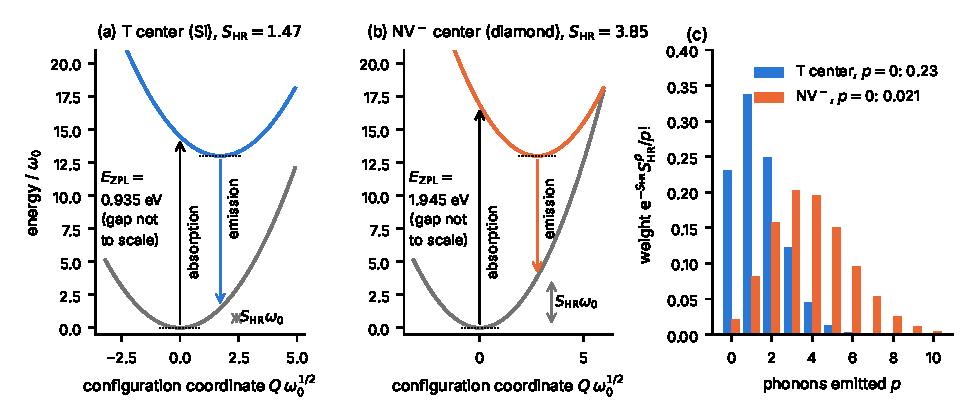
\includegraphics[width=\linewidth]{figures/ch07/fig7_5.pdf}
  \caption{Configuration-coordinate diagrams of (a) the T center in silicon, $E_{\mathrm{ZPL}} = \SI{0.935}{eV}$, $S_{\mathrm{HR}} = 1.47$ (from the measured zero-phonon fraction 0.23~\cite{bergeron2020silicon}), and (b) the negatively charged nitrogen--vacancy center in diamond, $E_{\mathrm{ZPL}} = \SI{1.945}{eV}$, $S_{\mathrm{HR}} = 3.85$~\cite{alkauskas2014first}. Each center is modeled by one effective mode of energy $\omega_0$, the same in both electronic states, in the Condon approximation; energies are in units of $\omega_0$ (\SI{64}{meV} for the nitrogen--vacancy center) and the coordinate in units of $\omega_0^{-1/2}$, \cref{eq:7.4-cc}. Gray: ground-state surface; colored: excited state, drawn with a reduced gap $E_{\mathrm{ZPL}}$ (not to scale). Arrows: vertical absorption from the ground minimum and emission from the excited minimum; the double arrow is the relaxation energy $S_{\mathrm{HR}}\omega_0$. (c) Zero-temperature weights of the emission lines with $p$ phonons emitted, $\ee^{-S_{\mathrm{HR}}}S_{\mathrm{HR}}^p/p!$; the zero-phonon line is $p = 0$.}
  \label{fig:7-cc}
\end{figure}

Comparing \cref{eq:7.4-zpl} with a luminescence spectrum needs one correction. The rate of spontaneous emission into a line of energy $E$ grows as $E^3|\vect{d}|^2$, with $\vect{d}$ the transition dipole, so a luminescence spectrum counts photons with the Franck--Condon weight times $E^3$~\cite[Eq.~(2)]{alkauskas2014first}. The sideband lies at lower energy and is suppressed by this factor, and the zero-phonon line takes a larger share of the photons than of the Franck--Condon weight:
\begin{equation}
  \frac{\text{photons in the zero-phonon line}}{\text{all photons}} = \frac{\ee^{-S_{\mathrm{HR}}}E_{\mathrm{ZPL}}^3}{\sum_p\ee^{-S_{\mathrm{HR}}}S_{\mathrm{HR}}^p(E_{\mathrm{ZPL}} - p\,\omega_0)^3/p!} ,
  \label{eq:7.4-photon}
\end{equation}
in the single-mode model. The correction is of order $3S_{\mathrm{HR}}\omega_0/E_{\mathrm{ZPL}}$, large when the relaxation energy is a sizable fraction of the line energy.

Computing these numbers is a supercell problem. $E_{\mathrm{ZPL}}$ is the difference of two total energies, each at its own relaxed geometry, with the excited state obtained by constraining the occupations of the defect orbitals; $S_{\mathrm{HR}}$ follows from the displacement between the two geometries projected on the vibrational modes, $S_{\mathrm{HR}} = \sum_k\omega_k\Delta Q_k^2/2$. A hybrid functional in a 512-atom cell puts the T-center line at \SI{985}{meV}, \SI{50}{meV} above the measurement~\cite{dhaliah2022first}, and the converged Huang--Rhys factor of the nitrogen--vacancy center is 3.67 against the measured 3.85~\cite[Sects.~4.2 and~4.3]{alkauskas2014first}.

\begin{workedexample}{Zero-phonon fractions}\label{we:7-zpl}
We compute the zero-phonon fractions of the T center and the nitrogen--vacancy center and check the second against its measured photon count.

\emph{T center.} Through \cref{eq:7.4-zpl}, the measured photon fraction 0.23 means $S_{\mathrm{HR}} = -\ln0.23 = 1.47$. The weights of the lines with 0, 1, 2 and 3 phonons are 0.23, 0.34, 0.25 and 0.12 (\cref{fig:7-cc}c): one photon in four is in the zero-phonon line, and one in three has emitted exactly one phonon. Read through \cref{eq:7.4-photon}, the photon fraction slightly overstates the Franck--Condon weight. The bound on the correction, $3S_{\mathrm{HR}}\omega_0/E_{\mathrm{ZPL}}$ with $\omega_0$ at most the \SI{64}{meV} of the silicon optical phonon (\cref{sec:5.3}), is $3\times1.47\times0.064/0.935 = 0.30$, so the photon count shifts $S_{\mathrm{HR}}$ by at most 0.30. The true Huang--Rhys factor lies between 1.47 and about 1.8, and the zero-phonon weight between 0.23 and 0.17.

\emph{Nitrogen--vacancy center.} With $S_{\mathrm{HR}} = 3.85$, \cref{eq:7.4-zpl} gives $w_{\mathrm{ZPL}} = \ee^{-3.85} = 0.021$, ten times less than the T center. The line with three phonons is the strongest, at 0.20. The relaxation energy is $S_{\mathrm{HR}}\omega_0 = 3.85\times\SI{64}{meV} = \SI{0.246}{eV}$, so absorption peaks near \SI{2.19}{eV} and emission near \SI{1.70}{eV}, a Stokes shift of \SI{0.49}{eV}.

\emph{The photon check.} In \cref{eq:7.4-photon}, with $\omega_0/E_{\mathrm{ZPL}} = 0.064/1.945 = 0.0329$, the Poisson average of $(1 - 0.0329\,p)^3$ is
\begin{equation*}
  1 - 3(0.0329)S_{\mathrm{HR}} + 3(0.0329)^2(S_{\mathrm{HR}} + S_{\mathrm{HR}}^2) - (0.0329)^3(S_{\mathrm{HR}} + 3S_{\mathrm{HR}}^2 + S_{\mathrm{HR}}^3) = 0.677 ,
\end{equation*}
from the first three moments of the Poisson distribution. The photon fraction is then $0.0213/0.677 = 0.031$. The measured share of the zero-phonon line in the emission is \num{0.032}~\cite[Sect.~3]{alkauskas2014first}. Taken at face value, $-\ln0.032$ would give $S_{\mathrm{HR}} = 3.44$, an underestimate by 0.4 that the single-mode model attributes entirely to the $E^3$ weighting.

\emph{Detection fraction.} A detector that reads a color center through its zero-phonon line collects a quarter of the T center's photons and three percent of the nitrogen--vacancy center's. The rest come out in the sideband, spread over several phonon energies below the line, where a narrow filter rejects them together with the background.
\end{workedexample}

\subsection{Displacement thresholds and Frenkel pairs}

A silicon atom struck along $\langle111\rangle$ with \SI{12.5}{eV} can leave its site for good; struck along $\langle100\rangle$, it needs \SI{20}{eV}~\cite[Table~IV]{holmstrom2008threshold}. Below these energies the atom swings out, hands its energy to its neighbors and returns. The difference between the two outcomes is a statement about the energy surface $E^{\mathrm{ad}}(u)$ of \cref{sec:5.1}. The perfect crystal is its lowest minimum, but the surface has many other local minima, separated from it by barriers of several eV. A \emph{vacancy} is an empty lattice site. An \emph{interstitial} is an extra atom between the sites; in silicon it can sit at the tetrahedral or the hexagonal interstitial site or share a site with a lattice atom as a split $\langle110\rangle$ dumbbell. An atom moved from its site into an interstitial position leaves a vacancy behind, and the two together are a \emph{Frenkel pair}. Each configuration costs a formation energy, the height of its minimum above that of the perfect crystal. Density-functional calculations put the isolated vacancy at 3.4 to \SI{3.9}{eV}, the interstitials at 4.7 to \SI{5.8}{eV}, and the most stable close Frenkel pair, a tetrahedral interstitial \SI{4.7}{\angstrom} from its vacancy, at 6.8 to \SI{7.5}{eV}~\cite[Table~III]{holmstrom2008threshold}. A cheaper minimum exists without any vacancy: the \emph{bond defect}, a local rearrangement of bonds, at 2.6 to \SI{3.0}{eV}.

The \emph{displacement threshold energy} $E_{\mathrm{d}}(\hat{\vect{r}})$ is the smallest kinetic energy that, given to one atom in the direction $\hat{\vect{r}}$, leaves the crystal in a minimum other than the perfect one once the motion has died out,
\begin{equation}
  E_{\mathrm{d}}(\hat{\vect{r}}) = \min\bigl\{E_R :\ \text{the trajectory on } E^{\mathrm{ad}} \text{ from } (E_R, \hat{\vect{r}}) \text{ ends in a defect}\bigr\} .
  \label{eq:7.4-Ed}
\end{equation}
It is not the formation energy of the pair it creates, and it is always larger. The struck atom must squeeze between its neighbors, over a barrier that lies on its path and not at the end points. It loses energy to every atom it pushes. And if it stops too close to its own vacancy, the pair recombines and the crystal returns to its minimum. $E_{\mathrm{d}}$ therefore depends on the direction, through the open and closed channels of the lattice, and on the path of the whole collision. It is computed by molecular dynamics: a single trajectory on $E^{\mathrm{ad}}$ for each direction and energy, repeated over many directions (\cref{app:E.11}).

For silicon, density-functional molecular dynamics finds the lowest threshold, \SI{12.5}{eV}, along $\langle111\rangle$, where the struck atom pushes its neighbor into the tetrahedral site in a short replacement sequence; \SI{20}{eV} along $\langle100\rangle$; and \SI{36}{eV} for a Frenkel pair averaged over all directions~\cite[Table~IV]{holmstrom2008threshold}. Electron-irradiation experiments see damage set in at $12.9 \pm \SI{0.6}{eV}$~\cite{loferski1958radiation}, in agreement with the minimum. In most directions a bond defect forms at a lower energy than a Frenkel pair, and the average threshold for a defect of either kind is \SI{24}{eV}~\cite[Table~IV]{holmstrom2008threshold}. Which number is quoted depends on what is counted: a count of vacant and doubly occupied lattice sites sees the Frenkel pair but not the bond defect. The classical Stillinger--Weber potential, used for the large statistical scans, overshoots the density-functional thresholds along $\langle111\rangle$ by 4 to \SI{6}{eV}~\cite[Sect.~IV]{holmstrom2008threshold}, and its thresholds range from 17.5 to \SI{63.5}{eV} over all directions~\cite{kadribasic2018directional}.

The threshold is not the energy that stays in the crystal. A close Frenkel pair stores \SIrange{6.8}{7.5}{eV}, about half of the minimum threshold and a fifth of the average one; the rest of the recoil energy becomes heat within picoseconds. The stored energy is invisible to a calorimeter that measures the heat. It is a missing part of the deposit, and \cref{sec:19.4} turns this into the defect fraction of a recoil and the bounds that calibration data put on it. For dark matter, only heavy enough particles can reach these thresholds at all. By \cref{eq:1.3-ERmax}, with the silicon nuclear mass $M = \SI{26.16}{GeV}$ and $v_{\mathrm{max}} = \num{2.650e-3}$, a recoil of \SI{12.5}{eV} needs $\mchi \ge \SI{0.153}{GeV}$, and one of \SI{36}{eV} needs \SI{0.26}{GeV}. Since $E_{\mathrm{d}}$ depends on the direction of the recoil relative to the crystal axes, the rate of defect creation near threshold carries the direction of the dark-matter wind, a handle for directional detection~\cite{kadribasic2018directional}.

\subsection{Defects as targets and readouts}

A shallow donor is a target in its own right, with the threshold and the kinematic match of \cref{we:7-sip}. Its weakness is the number of electrons. A donor density of \SI{e15}{cm^{-3}} is five parts in $10^{9}$ of the valence electrons of silicon, \SI{2.0e23}{cm^{-3}}, and the interaction with the bound electron is screened by the same $\varepsilon_0$ that makes it shallow. The rate requires the response of the donor to the dark-matter operators, with its valleys and central cell, which \cref{sec:16.5} derives.

A color center is a target with a level inside the gap and a readout with an optical line. As a target, the T center needs $\mchi \ge 2\times\SI{0.935}{eV}/v_{\mathrm{max}}^2 = \SI{0.266}{MeV}$, below the \SI{0.333}{MeV} of the silicon gap, because its excitation sits \SI{0.24}{eV} below the band edge. The momentum at threshold is $2E_{\mathrm{ZPL}}/v_{\mathrm{max}} = \SI{0.71}{keV}$, and a transition at that momentum needs states localized to about $1/\SI{0.71}{keV} = \SI{2.8}{\angstrom}$, which the deep levels of the center are. The nitrogen--vacancy center needs \SI{0.554}{MeV} and \SI{1.47}{keV}. As a readout, the zero-phonon fraction sets how many of a center's photons survive a narrow filter (\cref{we:7-zpl}), and the spins of both centers can be polarized and read optically. As a final state, a color center can be created by a nuclear recoil, by a displacement or by the capture of a vacancy, and the threshold $E_{\mathrm{d}}$ sets where that begins (\cref{sec:16.6}).

A displaced atom, finally, is a long-lived final state. The Frenkel pair or the bond defect left by a recoil persists as long as its barriers allow. At \SI{10}{mK} the Boltzmann factor for crossing a barrier of \SI{0.1}{eV} is $\ee^{-1.2\times10^5}$, and only tunneling or the phonons of a later event move the defect.

\section*{Summary}

The Coulomb interaction does not act on spin, yet it couples spins, and in NiO it orders them below \SI{523}{K} (\cref{sec:7.1}). At low energy only the spins remain, coupled by the Heisenberg model, and in NiO one exchange constant, the measured $J_2 = \SI{19.01}{meV}$ between next-nearest nickel neighbors, sets the scale. In an antiferromagnet the exchange creates spin deviations in pairs, a bosonic Bogoliubov transformation removes the pair terms, and the dispersion becomes linear, with a measured maximum of ${\sim}\SI{117}{meV}$ in NiO. Density-functional values of $J_2$ spread from 11 to \SI{27}{meV}, and that spread is the theory uncertainty for a magnet without neutron data. A dark-matter particle that couples to the electron spin acts through the spin density $\vect{s}_e(\vect{q})$, and its one-magnon response follows from the Bogoliubov coefficients.

Phonon exchange makes electrons near the Fermi surface attract each other, with the dimensionless strength $\mathcal{N}_{\mathrm{F}}V_{\mathrm{BCS}} = \lambda_{\mathrm{ep}}$, reduced by the quasiparticle residue and the Coulomb pseudopotential (\cref{sec:7.2}). The excitations of the BCS state are Bogoliubov quasiparticles of energy $(\xi_{\vect{k}}^2 + \Delta_{\mathrm{BCS}}^2)^{1/2}$, and a probe that conserves the electron number creates them in pairs, so the threshold is $2\Delta_{\mathrm{BCS}}$. Independent quasiparticles, however, do not conserve charge; the conserving response of the Nambu formalism removes the defect through the phase mode of the condensate and satisfies the density Ward identity. For aluminum the measured critical temperature fixes $\Delta_{\mathrm{BCS}} = \SI{0.179}{meV}$, a threshold of \SI{0.36}{meV} and a threshold mass of \SI{0.10}{keV}.

Near a point where two bands nearly touch, the $\vect{k}\cdot\vect{p}$ expansion becomes a Dirac Hamiltonian, with the velocity $v_{\mathrm{D}}$ in place of the speed of light and the half-gap $\Delta_{\mathrm{D}}$ in place of the mass (\cref{sec:7.3}). A cone with $v_{\mathrm{D}} > v_{\mathrm{max}}$ cannot be excited by scattering at any mass, while a slow cone opens the target to light particles: \SI{8.0}{keV} for ZrTe$_5$-like parameters. The Dirac electrons screen on top of a background dielectric constant $\varepsilon_{\mathrm{bg}}$, with the effective coupling $\tilde\alpha = \alpha/(\varepsilon_{\mathrm{bg}}v_{\mathrm{D}})$, and a gapless cone has no screening length.

Defects put levels inside the gap of silicon itself (\cref{sec:7.4}). Effective-mass theory binds every shallow donor by \SI{31.3}{meV} at the liquid-helium dielectric constant 11.4, and the central-cell correction of the $s$-like ground state, \SI{14.3}{meV}, brings phosphorus to its measured \SI{45.6}{meV}, which opens silicon to dark matter of \SI{13}{keV}. A color center couples its electronic transition to local vibrations, and the measured zero-phonon fraction $\ee^{-S_{\mathrm{HR}}} = 0.23$ of the T center of silicon means $S_{\mathrm{HR}} = 1.47$. A recoiling atom that receives more than the displacement threshold, \SI{12.5}{eV} along $\langle111\rangle$ in silicon, leaves a Frenkel pair or a bond defect that stores energy no calorimeter sees. \Cref{chap:8} gathers the responses of all these targets, and those of the earlier chapters, into one framework for the rate.

\printbibliography[heading=subbibliography]
